\documentclass[a4paper, 12pt, abstracton]{scrartcl}
\usepackage[utf8]{inputenc}     % keyboard import
\usepackage[UKenglish]{babel}   % keyboard english
\usepackage{siunitx}            % correct presentation of numbers and units
\usepackage{lmodern}            % other caracter type
\renewcommand{\familydefault}{\sfdefault} % man kann neue Befehle so definieren
%\newcommand{\unit}[1]{\ensuremath{\, \mathrm{#1}}}
\newcommand{\degree}{\ensuremath{^\circ}}
\usepackage{amssymb, amsmath, cancel, ulem, graphicx, float, tabularx, multirow, bm}
\usepackage{braket}     % Für QT
\usepackage{verbatim}
\usepackage{caption}
\usepackage{subcaption}
\usepackage{mathtools}
\usepackage{tablestyles}
\usepackage{enumitem}
\usepackage{tikz}
\usepackage{graphicx}
\usepackage{fixltx2e}	% Um Text tief zu stellen
\usepackage{booktabs}	% Tabellenformatierung
\usepackage{pdfpages}	% to include PDFs
\usepackage{listings}
\usepackage{color} %red, green, blue, yellow, cyan, magenta, black, white
\definecolor{mygreen}{RGB}{28,172,0} % color values Red, Green, Blue
\definecolor{mylilas}{RGB}{170,55,241} % ?
\usepackage{commath}
\usepackage{nameref}
\usepackage{wrapfig}
\usepackage{breakurl}
\usepackage{url}
\usepackage{listings}
\usepackage[utf8]{inputenc} % Umlaute
\usepackage{hyperref}
\usepackage{chemist} % Für chemische Formeln noch anschauen!
\usepackage[noabbrev]{cleveref}
\newcommand{\sectionbreak}{\clearpage} % jedes Kapitel auf separate Seite starten
\renewcommand{\UrlFont}{\ttfamily\footnotesize} % font size url verkleinern

\usepackage[font=normalsize,labelfont=bf]{caption} % setzten der Schriftgrösse von caption
%\usepackage[font=scriptsize,labelfont=bf]{subcaption} % setzten der Schriftgrösse von subcaption

\DeclareCaptionFont{normalsize}{\normalsize\fontfamily{ptm}}
\captionsetup{textfont={normalsize}}

\usepackage{textgreek}
\usepackage{etoolbox}
\AtBeginEnvironment{tabular}{\normalsize\fontfamily{ptm}\selectfont} % Setzt Schriftart auf Times NewRoman

\setlength\parindent{0pt}
\setlength{\parskip}{6pt}

% For Bibliography
\usepackage[nottoc]{tocbibind}
\usepackage[square,numbers]{natbib}	% Für Biblio in Inhaltsverzeichnis ein
\bibliographystyle{abbrvnat}		% Typ wie Bibliography dargestellt wird.

\usepackage{times}					% Packet für Schriftart times

% Kopf-/Fusszeile
\usepackage{fancyhdr}   \pagestyle{fancy}
\lhead{} \chead{} \rhead{\leftmark}		% \leftmark = Name of the chapter
\lfoot{} \cfoot{\thepage}	% \thepage = page number at this position
\renewcommand\headrulewidth{2pt}
\renewcommand\footrulewidth{0.4pt}
\newcommand{\notes}[1]{{\color{red}{#1}}}
%\newcommand{\notes}[1]{} To delet all comments

	

\begin{document}
\renewcommand{\arraystretch}{1.5} % Macht Abstand der einzelnen Zeilen in einer Tabelle grösser
\fontfamily{ptm}\selectfont			% Setzt Schriftart auf Times NewRoman

\begin{titlepage}
	
	\begin{flushright}
		
\includegraphics[width=0.25\textwidth]{Bilder/logo-uni.jpg}\\[2cm]    
	\end{flushright}
	
	\begin{center} % Titelseite nach Unistandart einfügen ;)
		\huge \bfseries Application of Surface Physics for Instruments in Space Science\\[2cm]
		\Large Inauguraldissertation der Philosophisch-naturwissenschaftlichen Fakultät der Universität Bern\\[2cm]
		\Large vorgelegt von\\[0.1cm]
		\Large Martina Föhn\\[1cm]
		\Large 2021\\[1.5cm] % Date of the Defence
		\Large Leiter der Arbeit\\[0.1cm]
		\Large Prof. Dr. Peter Wurz\\[1cm]
		\Large Physikalisches Institut der Universität Bern\\
		
	\end{center}
\end{titlepage}

	%------------------------------------------------------------------------------
	
	\newpage
	\thispagestyle{empty}
	\null
	\newpage
	\pagenumbering{roman}
	\begin{abstract}

	\end{abstract}
%----------------------------------------------------------------------------------
	\newpage
	\thispagestyle{empty}
	\null
	\newpage

	\tableofcontents

	\newpage
	\thispagestyle{empty}
	\null
	\newpage
	
	\section*{List of Acronyms}
	% Noch alte Tabelle von Masterarbeit
	
	\begin{tabular}{>{\bfseries}l|l}
		
		BCVD  & Boron-doped Chemical Vapour Deposition \\ 
		
		DLC   & Diamond-Like Carbon surface \\ 
		
		EMG   & Exponentially Modified Gaussian \\ 
		
		ENA   & Energetic Neutral Atoms \\ 
		
		FWHM  & Full Width at Half Maximum \\ 
		
		IBEX  & Interstellar Boundary EXplorer \\ 
		
		ILENA & Imager for Low Energetic Neutral Atoms \\ 
		
		IMAP  & Interstellar Mapping and Acceleration Probe \\ 
		
		JNA   & Jovian Neutral Atom Analyser \\ 
		
		JUICE & JUpiter ICy moon Explorer \\ 
		
		L1    & Lagrange 1 \\
		
		LISM  & Local InterStellar Medium\\
		
		MCA   & MultiChannel Analyzer \\ 
		
		MCP   & MultiChannel Plate \\ 
		
		PA    & PostAcceleration voltage \\ 
		
		PEP   & Particle Environment Package \\
		
		RPA   & Retarding Potential Analyser \\
		
	\end{tabular}
	\newpage
	\thispagestyle{empty}
	\null
	\newpage
	
	\pagenumbering{arabic}

	% !TEX root = arbeit.tex
% Damit Latex weiss, wo die main Datei ist.
\section{Introduction}
	
	\subsection{Mission Introduction} % Search for a better title
	% Rockets:
	% https://www.grc.nasa.gov/www/k-12/TRC/Rockets/history_of_rockets.html
	
	Investigation of the stars and the night sky started a long time ago. Back then, the movement of the Sun, the Moon and the stars was used to derive time, for navigation and for religious rituals. First records of systematic observations of the night sky date back to the Assyro-Babylonians around 1000 BCE. In the third century BCE Greek astronomers tried to estimate the distances between the different cosmic objects with geometrical tools \cite{space_history}. The invention of telescopes in the early 17th century allowed then a closer look at the objects in the night sky and lead to the discovery of the Galilean moons' Io, Europa, Callisto and Ganymede by Galileo Galilei in 1610. Galileo discovered that these objects were orbiting around another object than the Sun, namely Jupiter. The invention of the first modern rockets during the cold war, opened the opportunity of on site exploration of solar system bodies.
	\begin{wrapfigure}{r}{0.5\textwidth}
		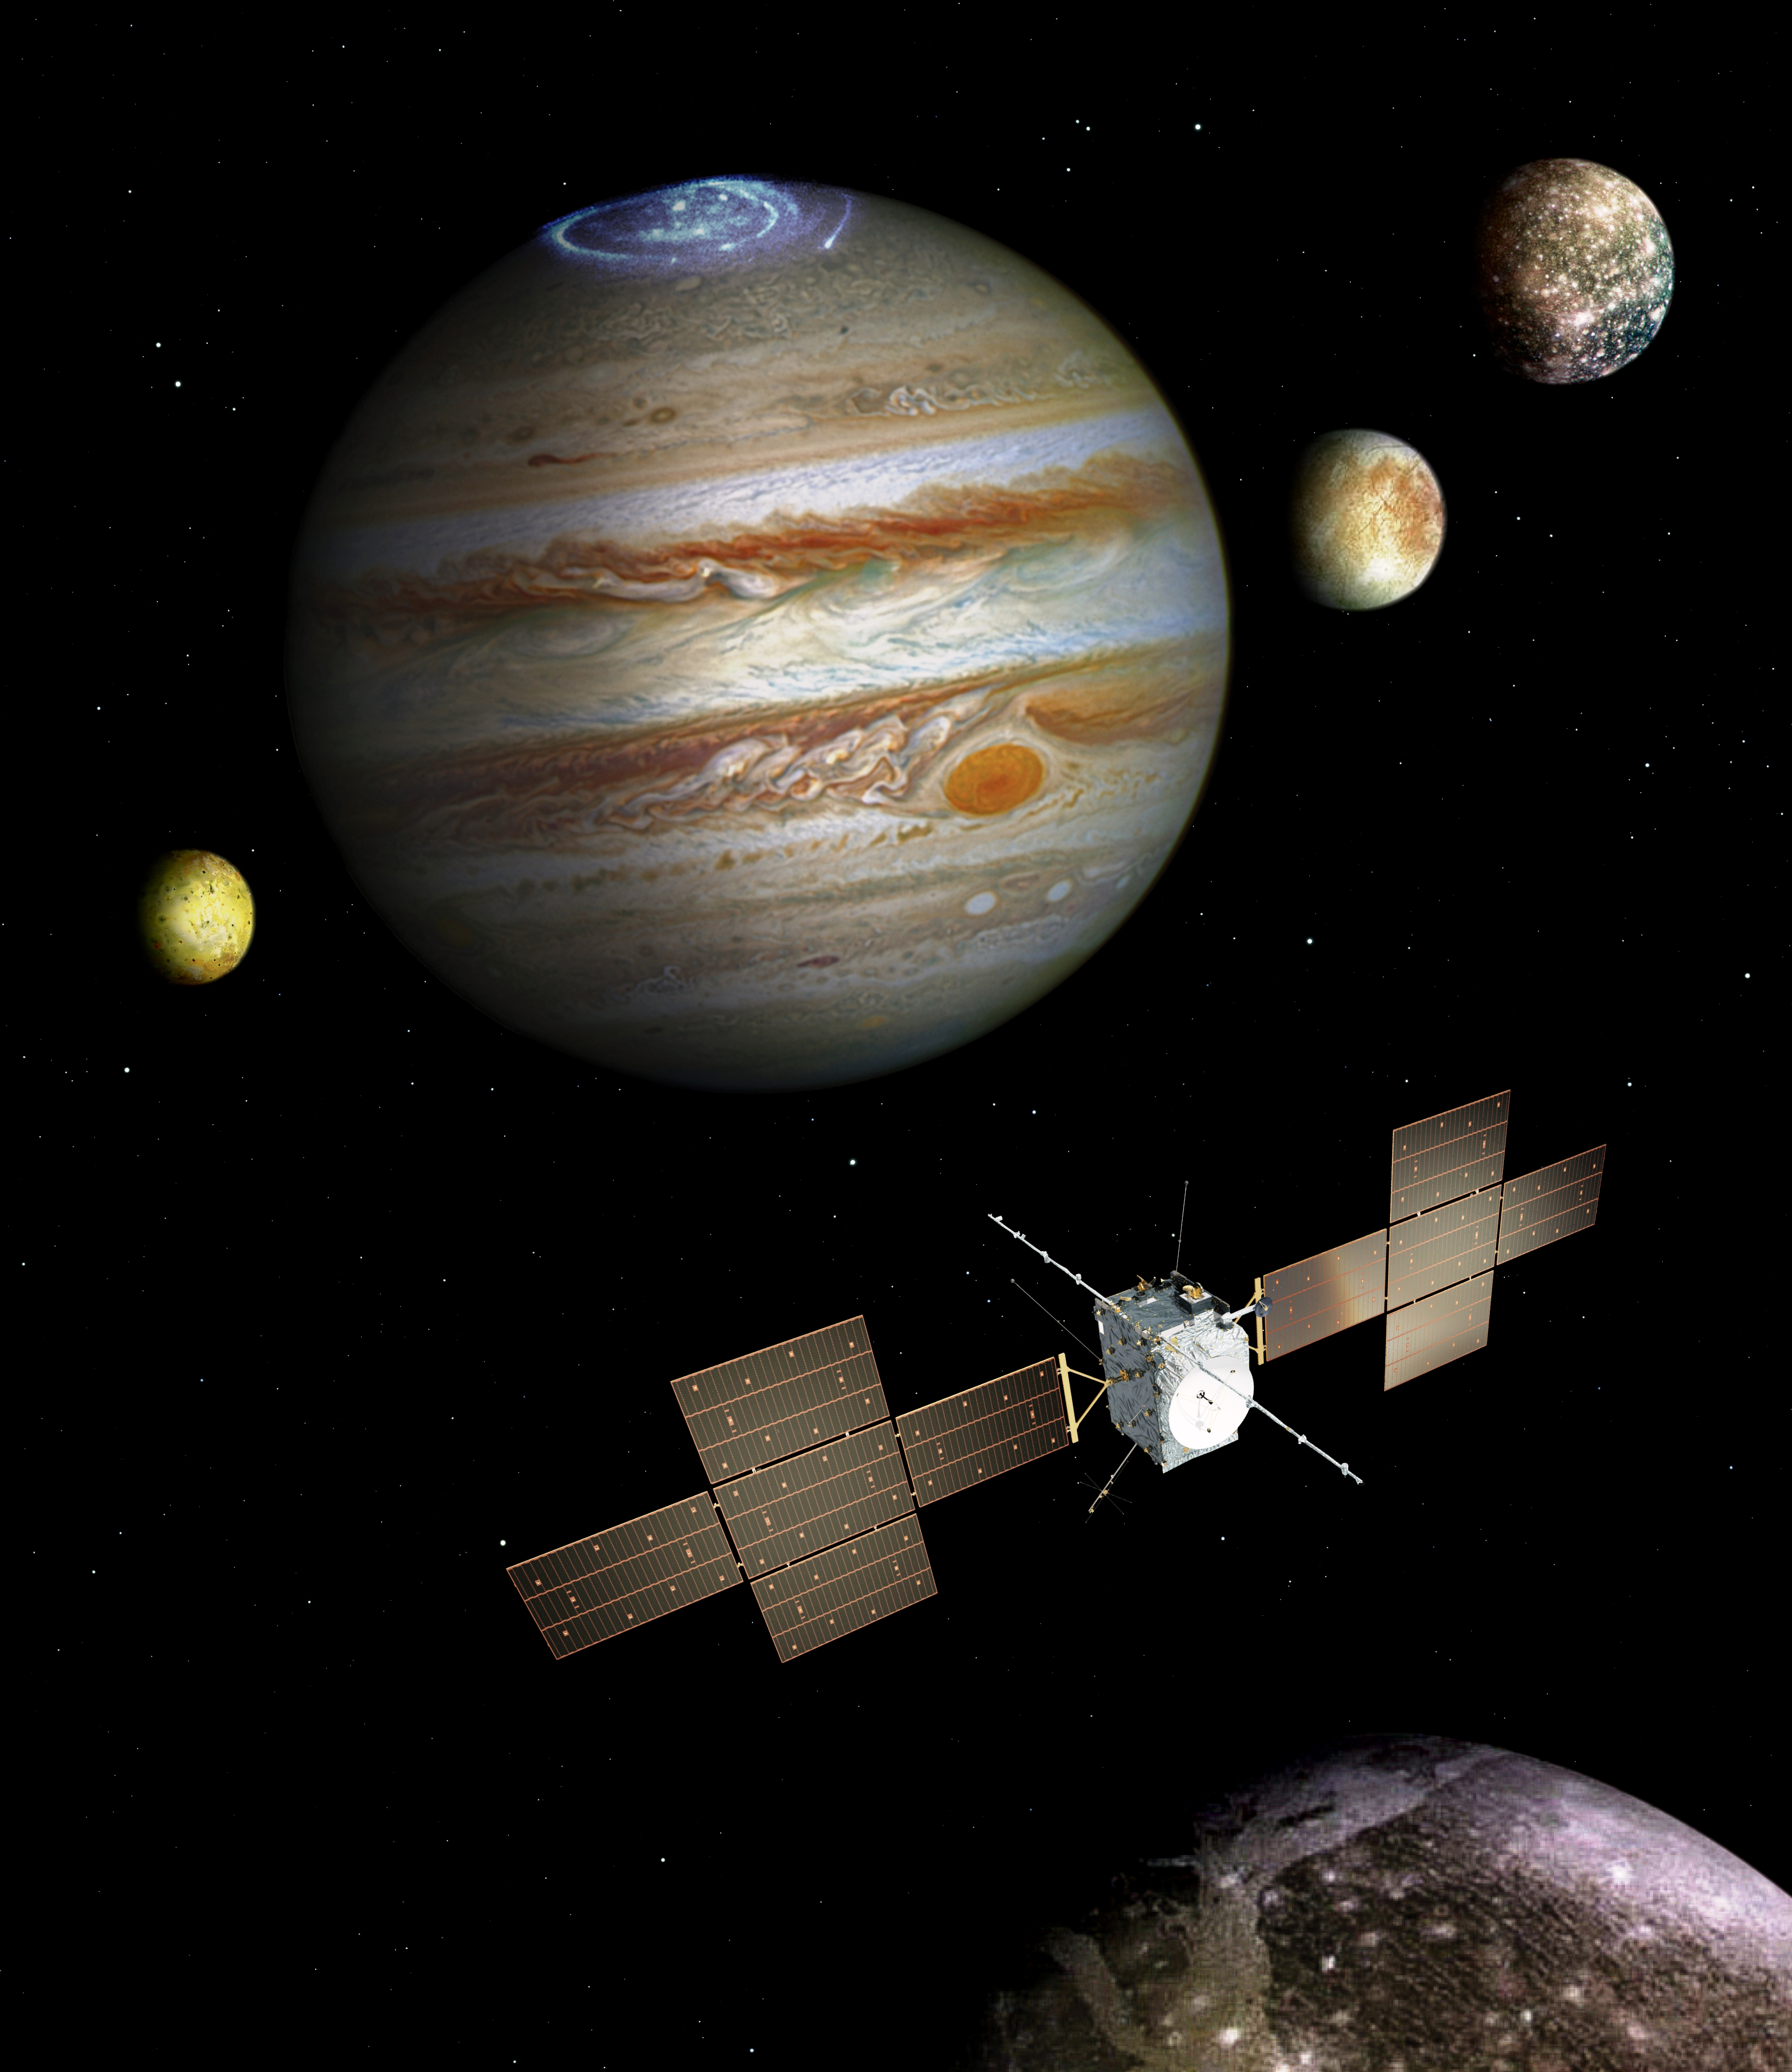
\includegraphics[width=\linewidth]{Bilder/Juice_mission.jpg}
		\caption{Artist impression of the Juice mission exploring the Jupiter system \cite{JUICE_Pic}.}
		\label{fig:JUICE}
	\end{wrapfigure}
	The data acquired through those in situ measurements gave further insight into the formation processes and history of our solar system. The missions Pioneer 10~\&~11 and Voyager 1~\&~2 were the first space missions, which took close images of Jupiter and its icy moons. They discovered Jupiter's ring system and detected more small moons of Jupiter than only the four big Galilean moons. The missions Galileo (1995-2003) and JUNO (2016-2025) were two missions specifically with the objective to further investigate Jupiter itself (JUNO) and its icy moons (Galileo) with the main outcome of giving strong evidence for salty subsurface oceans on the moons Europa, Ganymede and Callisto by measuring the induced magnetic fields. These oceans could be environments where life might be possible. In addition, the Galileo mission provided data that Ganymede has an intrinsic magnetic field interacting with the strong magnetic field of Jupiter \cite{Jupiter_SpaceMission}.\\
	The JUpiter ICy moons Explorer JUICE built by the European Space Agency ESA has the objective to further investigate Jupiter, its environment and its icy moons with regards to their potential of harbouring life. JUICE will characterise Jupiter as a planet, Jupiter's plasma environment and it will characterise Jupiter's icy moons Europa, Ganymede and Callisto. JUICE will characterise Jupiter's atmospheric dynamics, composition and chemistry and the atmosphere's vertical structure. It will characterise Jupiter's magnetosphere to understand the role of the moons as sources and sinks for the magnetospheric plasma. JUICE will study Jupiter's ring system, its small satellites and it will study Io's activity and surface composition with its remote sensing instruments.\\
	With regards to the icy moons, the main objectives are to characterise their potential subsurface oceans and their non-icy material. Europa consists mainly out of silicates with a water layer and an ice crust on top of that. Europa's surface is fairly young showing almost no impact craters, which implies that the icy crust frequently resurfaced similar to plate tectonics. Ganymede is until now the only satellite in our solar system known having an intrinsic magnetic field generated by a magnetic dipole field. Therefore, JUICE will investigate the interaction processes of that magnetic field with Jupiter's magnetic field because it is strong enough to successfully shield the moon against most of the plasma flow from Jupiter's magnetosphere. Callisto is the outer most of the Galilean moons and by far the most cratered. It lacks of small craters indicating some minor erosion processes. Compared to the other three Galilean moons, Callisto lacks any larger tectonic activity \cite{red_book}.\\
	\begin{figure}[H]
		\centering
		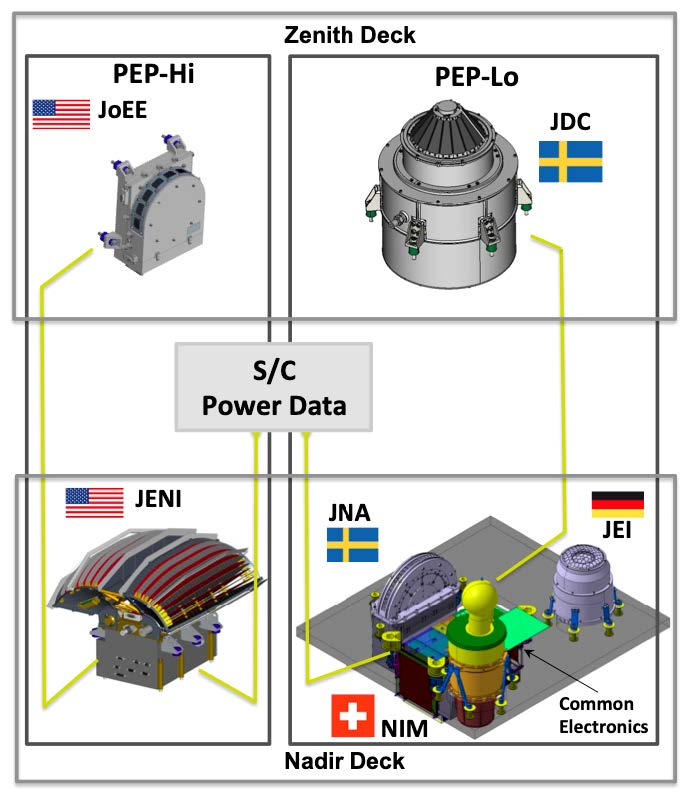
\includegraphics[width=.7\textwidth]{Bilder/PEP_Instruments.jpg}
		\caption{Sketch of the six PEP instruments and their organisation on the spacecraft \cite{PEP_inst}.}
		\label{fig:PEPInst}
	\end{figure}
	To fulfil the scientific goals, JUICE has an instrument suit consisting of 11 instruments on board ranging from cameras, spectrometers, magnetometers, to particle instruments, and gravity measurements. One of these instruments is the Particle and Environment Package System PEP (Fig.~\ref{fig:PEPInst}). The main focus of PEP is to characterise Jupiter's plasma environment and the composition of the icy moons' exospheres. Therefore, PEP has six instruments to measure neutral particles, ions and electrons with energies from thermal ($<$~5~eV) up to 5~MeV (ions) \cite{PEP_inst}. One of these six instruments is the Neutral Gas and Ion Mass Spectrometer NIM. The focus of NIM lays on the characterisation of the icy moons' exospheres and the detection of ions with an energy less than 10~eV to complete the plasma measurements for slow ions of the other PEP instruments. With the capability of measuring slow ions, NIM is able to detect a potential ionosphere of the icy moons \cite{Diss_Meyer}. NIM will be the first mass spectrometer taking in situ measurements of the icy moons exosphere. The exosphere is formed by particles released from the moons' surface by ion bombardment, sublimation and photon interaction processes. By sampling the exosphere, we get a deeper insight in the surface composition and the formation processes involved of the icy moons themself. For example, there are two major theories about when the icy moons were formed. One suggests that the icy moons' were formed in the protostar nebula of our solar system implying that the moons have a similar age as Jupiter. Another hypothesis suggests that the icy moons' were formed in the subnebula of Jupiter, implying that they are younger than Jupiter. By determining the particle density and isotope ratios of the detected species, we can distinguish between these two formation processes giving us a deeper insight in how our solar system was formed and which processes in the formation of the icy moons' are the most relevant \cite[and references therein]{Vorburger2015}.\\
	
	The instruments sent to space missions are highly customised to fulfil the specific requirements. For space missions, the instruments have to be small, light and low power consumptive. Especially for missions having targets in the outer solar system, such as JUICE with target Jupiter, power is a very limited resource. At Jupiter, the solar flux density is by a factor 25 lower than at Earth because Jupiter is five times farther away from the Sun than Earth. Therefore, missions flying to the outer solar system often use radioisotope thermoelectric generators (RTGs) as power sources instead of solar panels because they are longer lasting and provide more power. The biggest drawback is that they are very inefficient and produce a lot of heat, which cannot be used \cite{Power_Space}. Another main challenge is the harsh radiation environment of Jupiter. The penetrating particles lead to upset in the electronics and damage components. Therefore, a proper radiation shielding concept was necessary.\\

	NIM is a time-of-flight mass spectrometer with heritage from previous TOF instruments developed at the University of Bern. These are the RTOF/ROSINA/Rosetta \cite{Balsiger2007a,Scherer2006}, P-BACE/ MEAP \cite{Abplanalp2009a} and NGMS/Luna-Resurs \cite{Wurz2012264,Fausch_IEEE}. Mass spectrometers are single ion counting instruments. Therefore, they can estimate the density distributions of the measured species much more precisely than remote sensing instruments. The biggest advantages of time-of-flight mass spectrometers compared to other mass spectrometer types is that they are extremely robust from the mechanical point of view and have a better sensitivity than scanning instruments. Magnetic sectors are heavy and require high accuracy mechanics. Quadrupole mass spectrometers fulfil the requirements regarding size, weight and power but have a lower sensitivity than TOF instruments because to increase the mass resolution they loose sensitivity \cite{Quadrupol_WorkPrinc}. In addition, scanning instruments have a relatively long cadence \cite{MassSpec_Overview} leading to a bad spacial resolution during the flybys of the spacecraft on the icy moons. Therefore, TOF instruments are often used in space missions.\\
	NIM is designed to measure complex molecules up to 1000~u with a mass resolution up to m/$\Delta$m 1000 with a signal-to-noise ratio (SNR) of 6 decades. Based on present knowledge we expect in the icy moons exosphere only species with masses up to 100~u but with the ability to measure also species with higher masses, NIM is able to detect also potential organic compounds if they are present \cite{NIM_Req_dMSNR}. To separate species with such high masses, it requires a mass resolution of m/$\Delta$m 1000 to be able to distinguish between the different unit masses. With a SNR of 6 decades, NIM is able to measure down to partial pressures of 10\textsuperscript{--16}~mbar corresponding to a particle density of 1~cm\textsuperscript{--3}. During the flybys at the icy moons, the spacecraft velocity is 1--8~km/s. Depending on the mass of the particles, the highest energy they have is up to 100~eV which is the highest energy NIM has to deal with. NIM is designed to measure particles with thermal energy up to energies of 100~eV. NIM has an open and a closed source entrance for neutral particles and ions. Through the open source entrance slit, neutral particles and ions enter the ionisation region directly without interacting with the instrument structure. The closed source consists of an antechamber that thermalises incoming neutrals. Neutrals with higher speeds are therefore easier to detect than with the open source channel where particles enter the ionisation region with spacecraft velocity. As mentioned above, mass and power are for these missions very limited resources. The NIM ion-optical system has a mass of 3.13~kg from which 48~\% is shielding mass to shield the detector locally to reduce noise induced by high energetic particles originating from Jupiter's plasma environment. The primarily power allocated for the NIM instrument from the spacecraft is 18.5~W, including margin.

	\subsection{Thesis Outline}
	This thesis follows up the PhD thesis of Stefan Meyer \cite{Diss_Meyer}. At the end of his thesis, the NIM prototype was built and the flight design the NIM was almost completed.\\	
	The objective of this thesis was to finalise the design of the NIM flight model, to build and test the NIM Proto-Flight-Model (PFM) to deliver it to the JUICE spacecraft and to build and test the NIM Flight-Spare (FS) model, which stays on Earth as a ground reference. This required environmental tests of various flight subcomponents as they became available with finally testing the ion-optical system of the NIM PFM and FS model. Ion-optical simulations were performed to set constrains on the design of the flight power supplies as they were still under development during the early phases of this thesis.\\
	The thesis consists of three main parts: Chap.~\ref{sec:theory} shows theoretical analyses of key components of the NIM instrument such as the performance of the antechamber of the closed source. In addition, it completely presents the theoretical aspects needed to understand the performance results of the different subsystems presented in Chap.~\ref{sec:Exp}. Chap.~\ref{sec:setup} compares the design of the NIM prototype with the final flight design and shows the main differences between the two models. A special focus lays there in the improvements done on the design of the detector. Chap.~\ref{sec:Exp} sums up the performance tests of different subsystems partially tested stand alone (detector) or as part of the NIM Prototype (antechamber, ion-mirror). The chapter ends with performance tests of the two NIM flight models (PFM and FS).
	
	
	
	
	
	
	
	
	
	
	
	
	\newpage
	\thispagestyle{empty}
	\null
	\newpage
	% !TEX root = arbeit.tex
\section{Theory}

	\subsection{Requirements}
	% Mass, performance, Power consumption. (See latest references. Part of the introduction?)
	
	\subsection{Basic Theory about a TOF instrument}
	A time of flight mass spectrometer consists of, an ion-source, a mass analyser and a detector.\\
	
	\begin{figure}[htb] % Noch schauen, ob das noch verschoben wird.
		\centering
		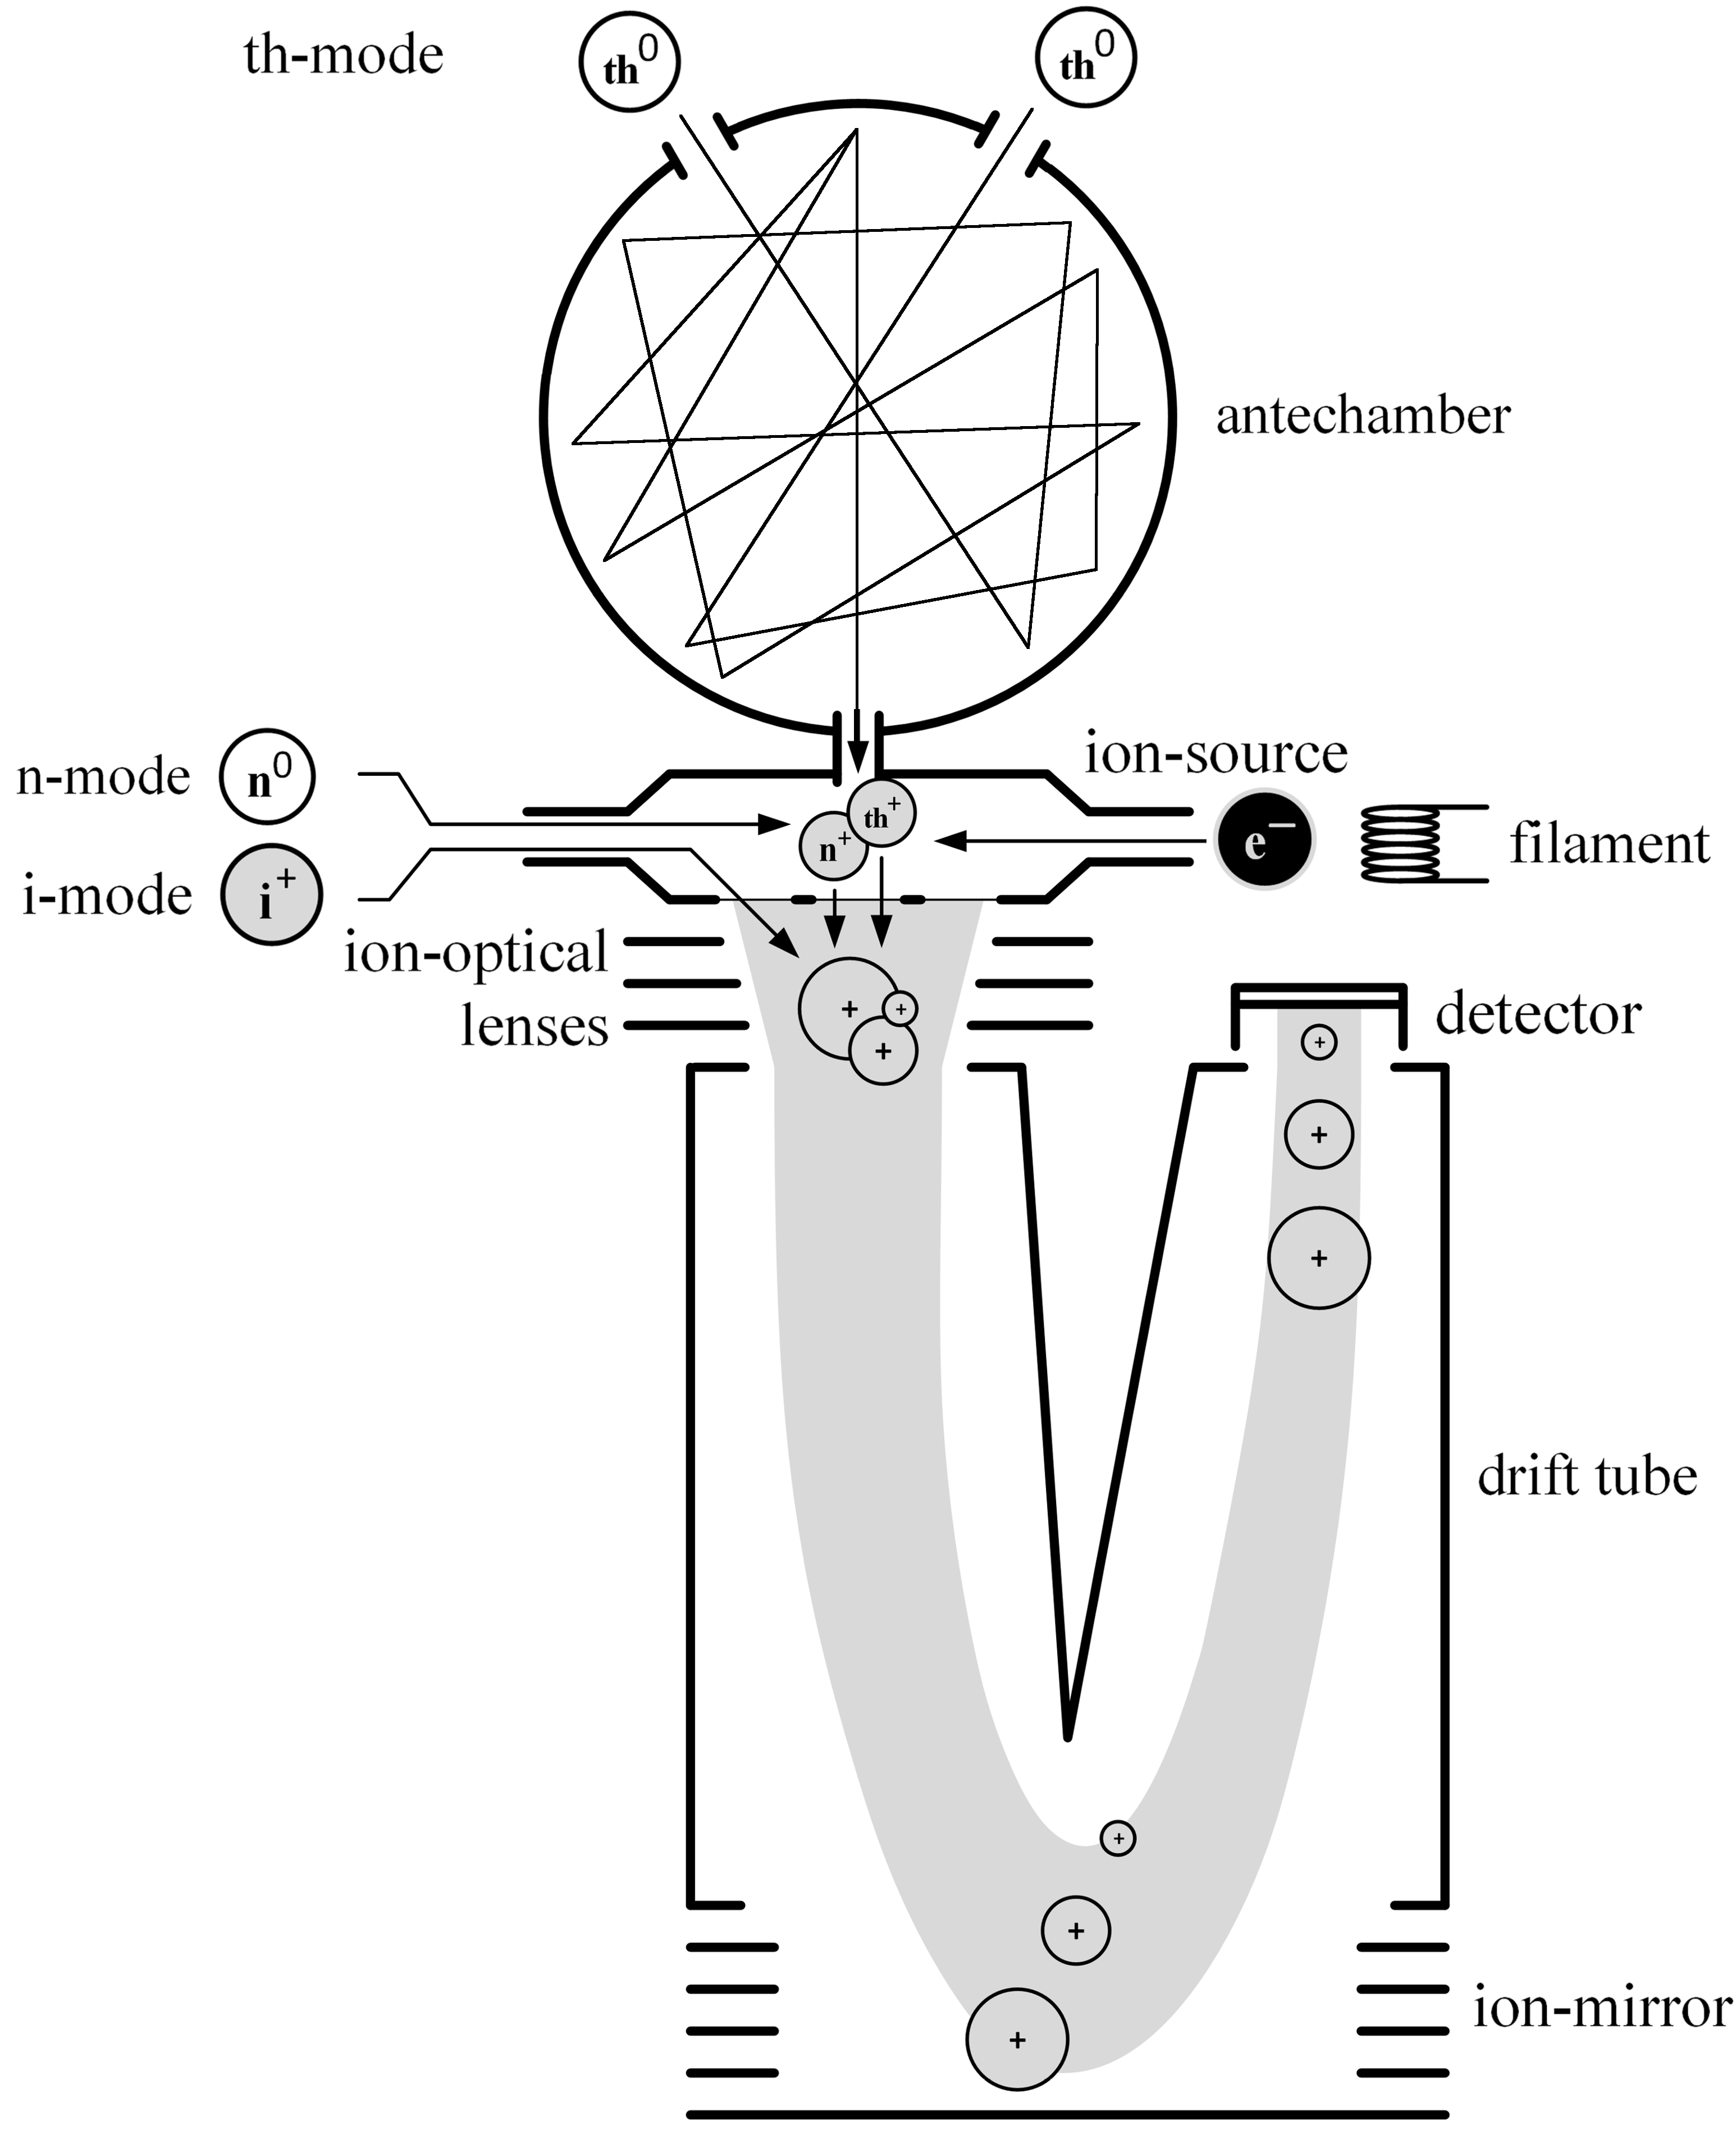
\includegraphics[width= 10cm]{Bilder/NIM_Sketch.png} % Bei Bild noch schauen, ob die Ränder drauf sind. Bei Zeiten noch Bild anpassen.
		\caption{Schematics of the NIM mass spectrometer. Adapted from \cite{Diss_Meyer}.}
		\label{fig:NIMSketch}
	\end{figure}

	%First overview and then go into the details.
	The NIM instrument is able to measure neutrals and ions. Neutral particles get ionised by electron ionisation. A filament is heated up until it emits electron. Ions enter the ion source directly.  % Noch genaue Formulierung nachschauen.
	All ions then get accelerated to the same energy and fly through the mass analyser. Light particles fly faster through the spectrometer than heavier ones. The different particle species arrive at different times at the detector. To enlarge the flight distance, an ion-mirror, which reflects the ions and leads them back to the detector. The used detector is a MCP detector. %Explain a little bit in more detail.
	
		\subsubsection{Ion-source}
		To calculate the number of ions produced in the ion source we use:
		\begin{equation}
		I_{ion} = \beta\cdot Q_{ion}\cdot L\cdot n\cdot I_{em}
		\end{equation}
		With $\beta$ the extraction efficiency which is 1, % Noch schauen auf welchen Wert wir diese setzen wollen. 1= sehr gute Quelle, 0.01 = 1mus/100mus = Pulslänge Pulser/ Länge 1 Zyklus. Noch diskutieren, welche Werte beta haben kann oder einfach etwas setzen? Da die ersten Messresultate gut sind, würde ich eher auf 1 setzen.
		$L$ as the effective ionising path in our case 4~\si{\milli\metre}, $n$ the particle density, $I_{em}$ the electron emission current from the filament and $Q_{ion}$ the ionising cross section. The cross sections of species used in our calibration can be found in table % Ref. auf Tabelle und nur auf Stefans Diss verweisen oder die 4 Originalpaper zusammen suchen.
		
		
		
		% Reference: Bieler Diss 2012, Wurz 2011, Scherer 1999, Meyer 2013 Data Analysis, Wells 2011
		% Ionisation efficiency
		% Description of how it works with the energies. Electric -> kinetic. Pulser. E = 1/2 mv^2 = qU
		% Time focusing?
		% Mass calibration t/dt -> m/dm.
		% SNR definition. Picture?
		% Sensitivity estimation. Nessesary? If so, part of SNR discussion.
		% MCP detector. Gain calculation. How the detecotr works. Didn't do anything for further developement...
		% Antchamber. Explanation of closed and open source. Field of view. Densitiy enhancement.
	
	
\begin{comment}
	
	Explain how a TOF works. Source, reflectron, detector.
	Explanation of the antechamber at the end after explaining the different parts.
	
	Detection efficiency Ionsource, MCP? -> y-Achse
	Mass Analyser, mass spectrometer. Most important formulas. dm/m = dt/t...
	Sensitivity
	Density enhancement -> explanation about closed and open source
	Sketch of the instrument
	Requirements: Power, mass, mass resolution,... (At the end or at the beginning. Introduction)
	
	
	Ionisationseffizienz/ Ionenproduktion der wichtigsten Gase. Detektionseffizienz hängt auch von Effizienz der MCPs ab... Erklären weshalb man die Achsenskalieruing braucht (entweder Counts oder die angepasste a.u. bei der Fläche und Counts/s für das Spektrum)
	
\end{comment}
		
	% Detectione efficiency Ionsource, MCP? -> y-Achse
	% Mass Analyser, mass spectrometer. Most important formulas. dm/m = dt/t...
	% Requirements: Power, mass, mass resolution,...
	\newpage
	% !TEX root = arbeit.tex
\section{Instrument}\label{sec:setup}
	% Pics with the lab power supply
	% \\titania.unibe.ch\UserHomes\foehn\My Documents\PhD\Fotos\[2021.02.04]FS_Sensor&Cube_in_Strofio
	\begin{figure}[h] % Prototype
		\centering
		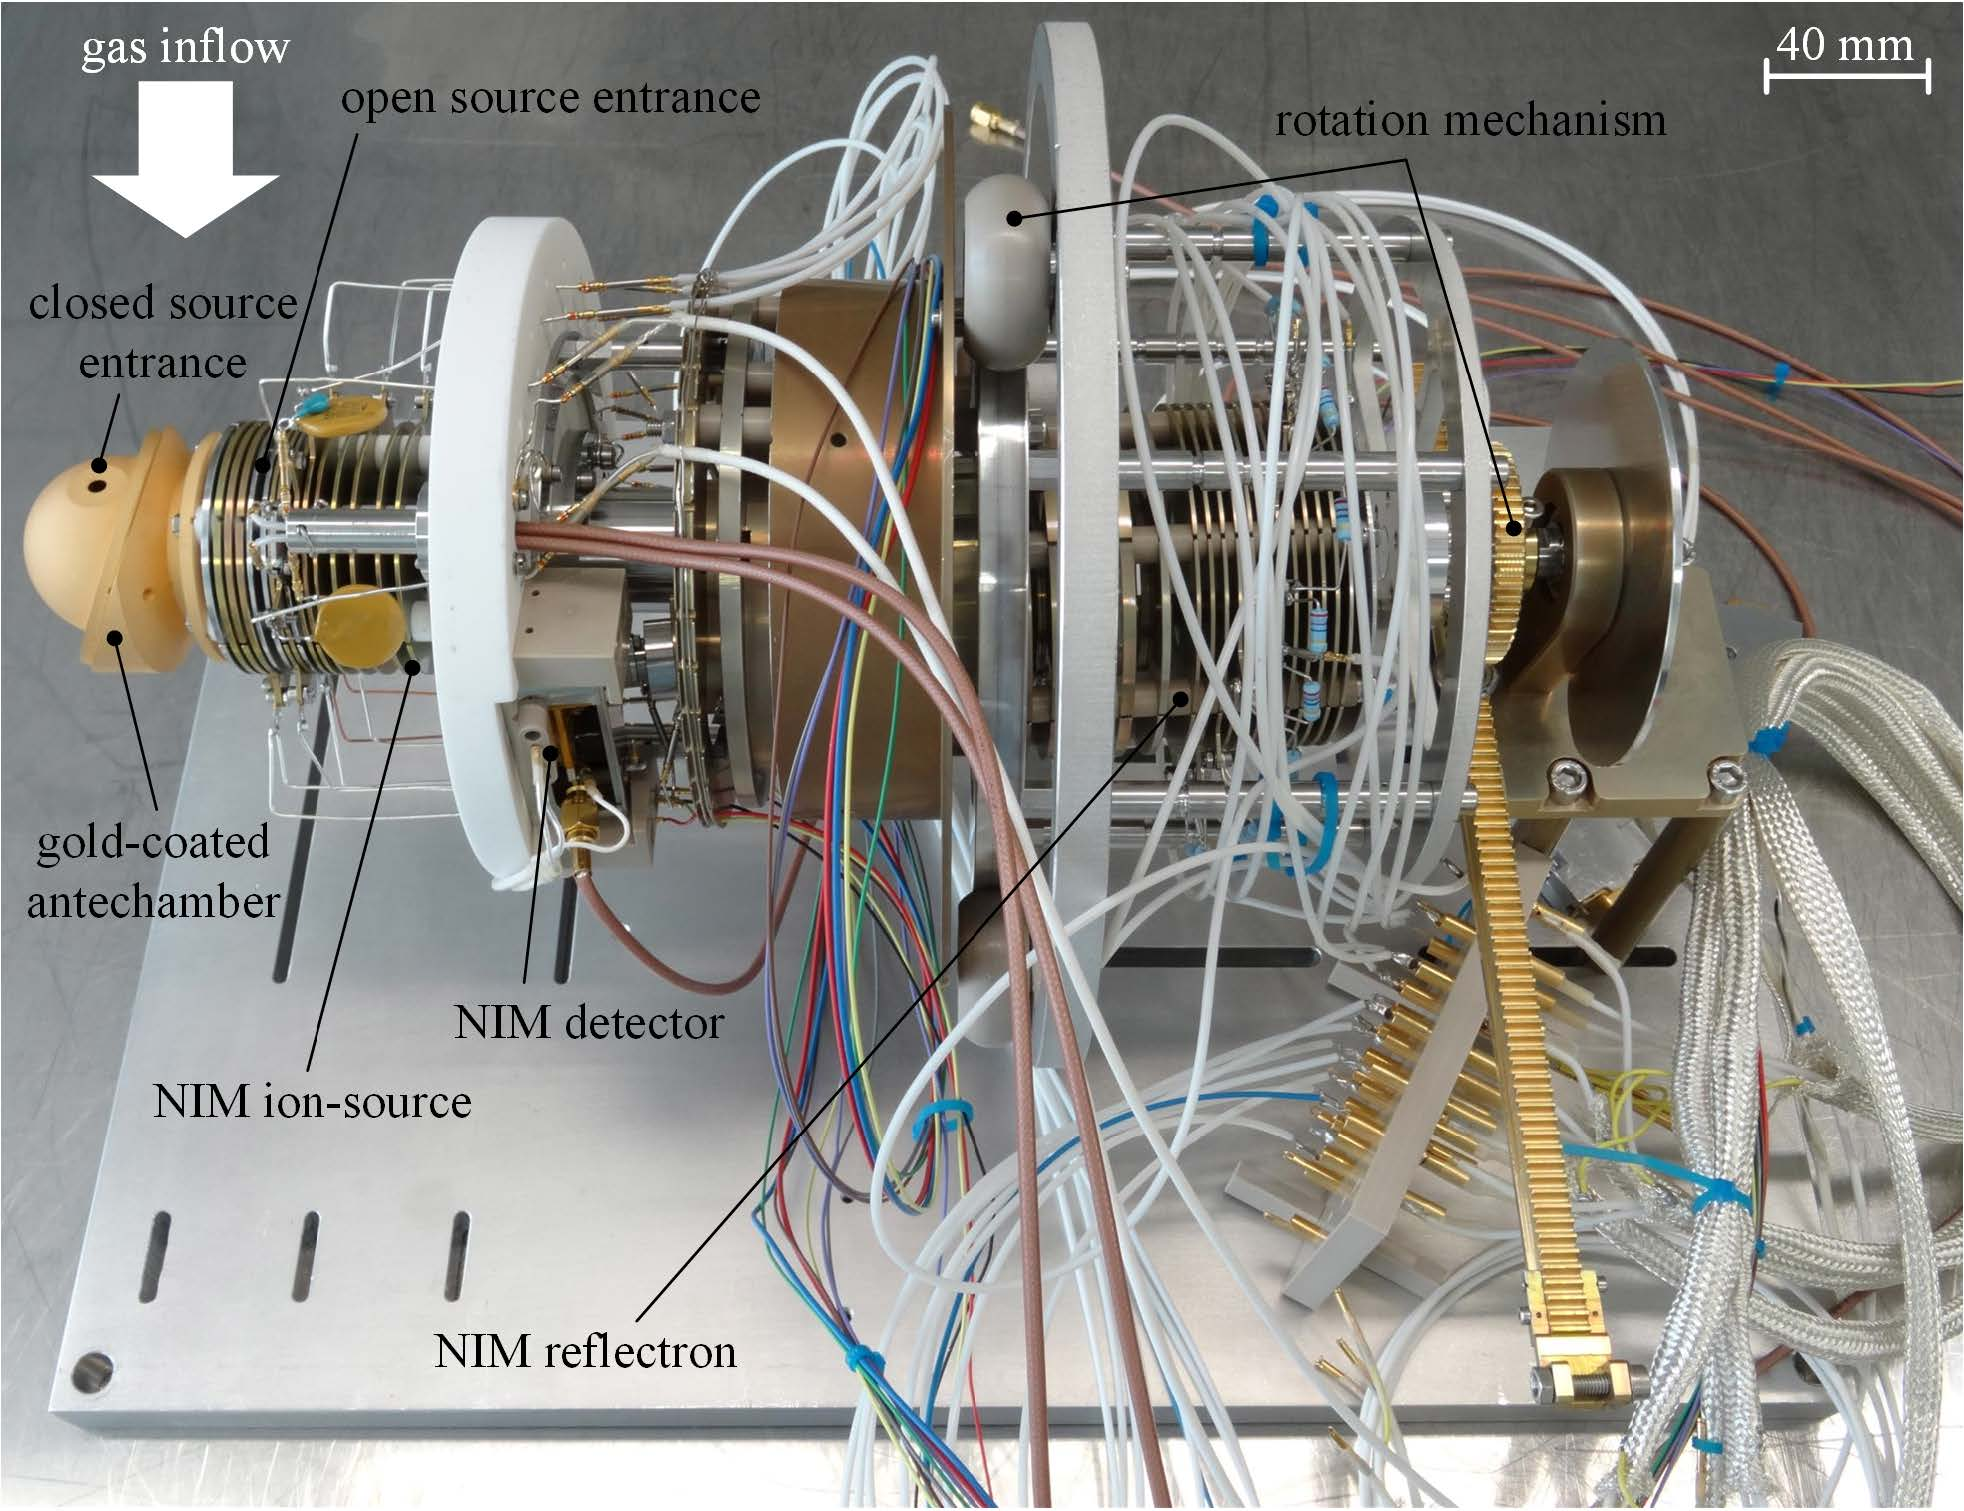
\includegraphics[width=\textwidth]{Setup/Prototype_totPic.jpg}
		\caption{NIM Prototype \cite{Diss_Meyer}.}
		\label{fig:SetupProto}
	\end{figure}
	\begin{figure}[h] % PFM Sensor
		\begin{subfigure}{0.5\textwidth}
			\centering
			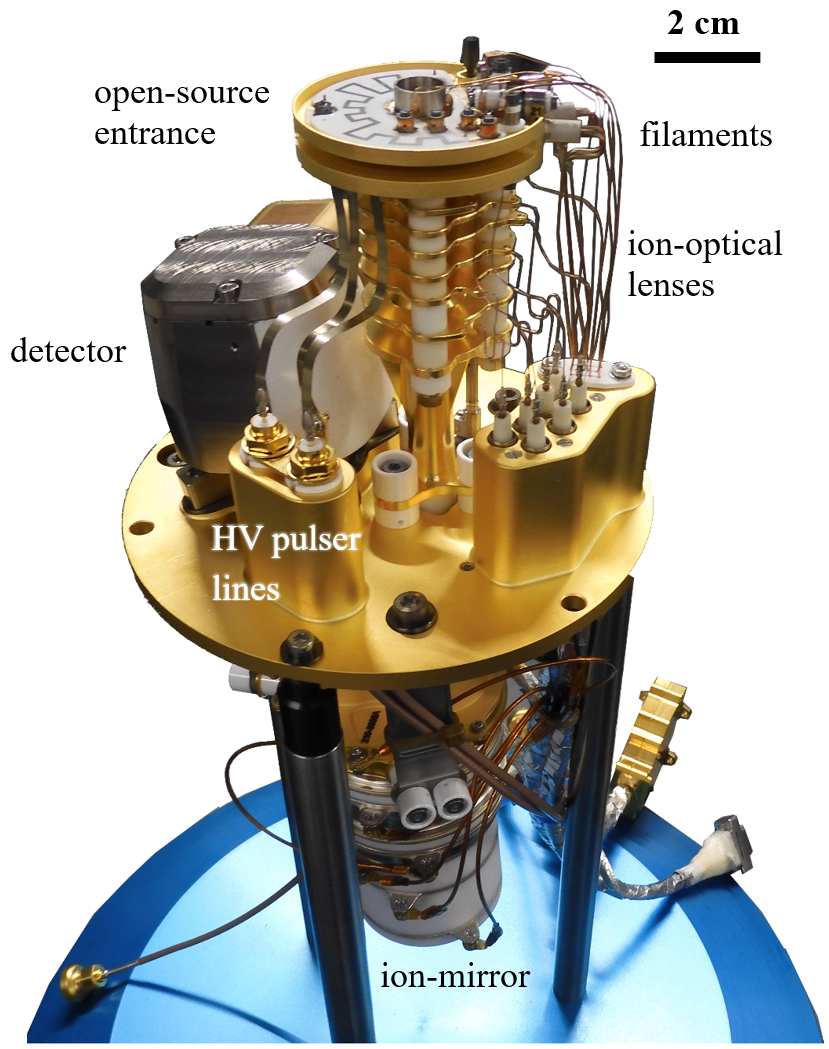
\includegraphics[width =.9\textwidth]{Setup/PFM_Sensor.png}
		\end{subfigure}
		\begin{subfigure}{0.5\textwidth}
			\centering
			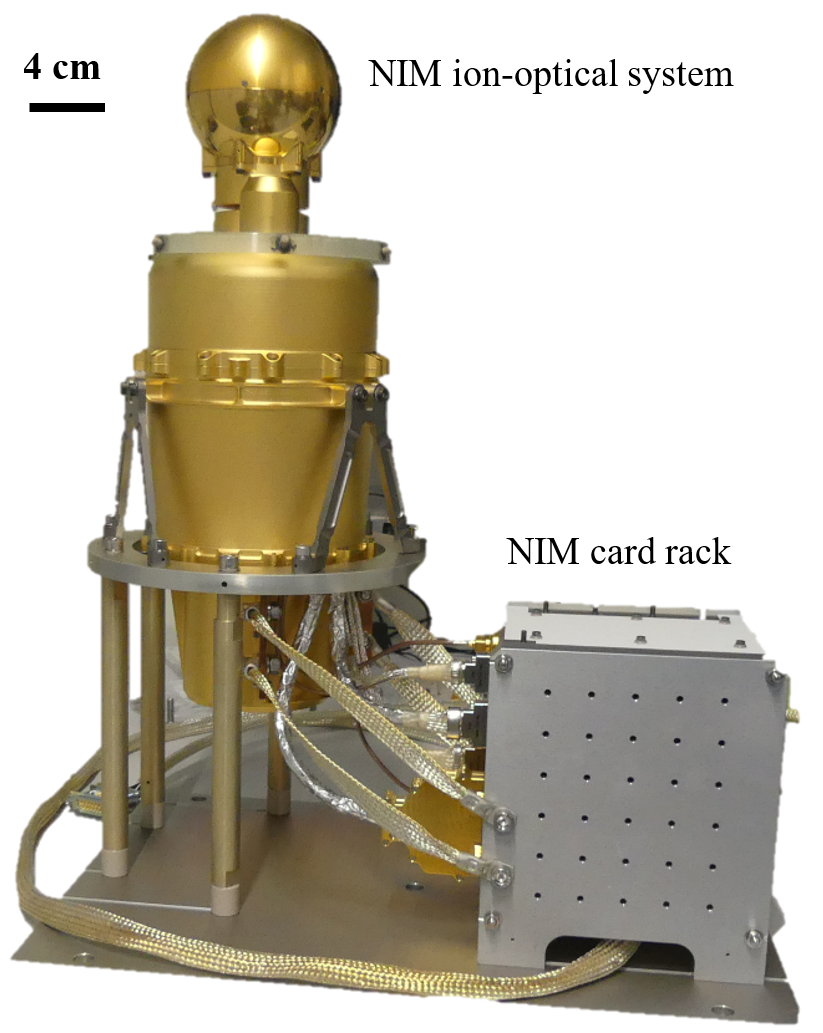
\includegraphics[width = \textwidth]{Setup/PFM_with_FlightEl.png}
		\end{subfigure}
		\caption{Left: NIM PFM ion-optical system without the closed-source antechamber. Right: NIM PFM ion-optical system with electronic box (card rack) attached \cite{Foehn2021}.}
		\label{fig:SetupPFM}
	\end{figure}
	\begin{figure}[h!] % Antechamber
		\begin{subfigure}{0.5\textwidth}
			\centering
			\includegraphics[width = .9\textwidth]{Setup/ProtoAnte.png}
		\end{subfigure}
		\begin{subfigure}{0.5\textwidth}
			\centering
			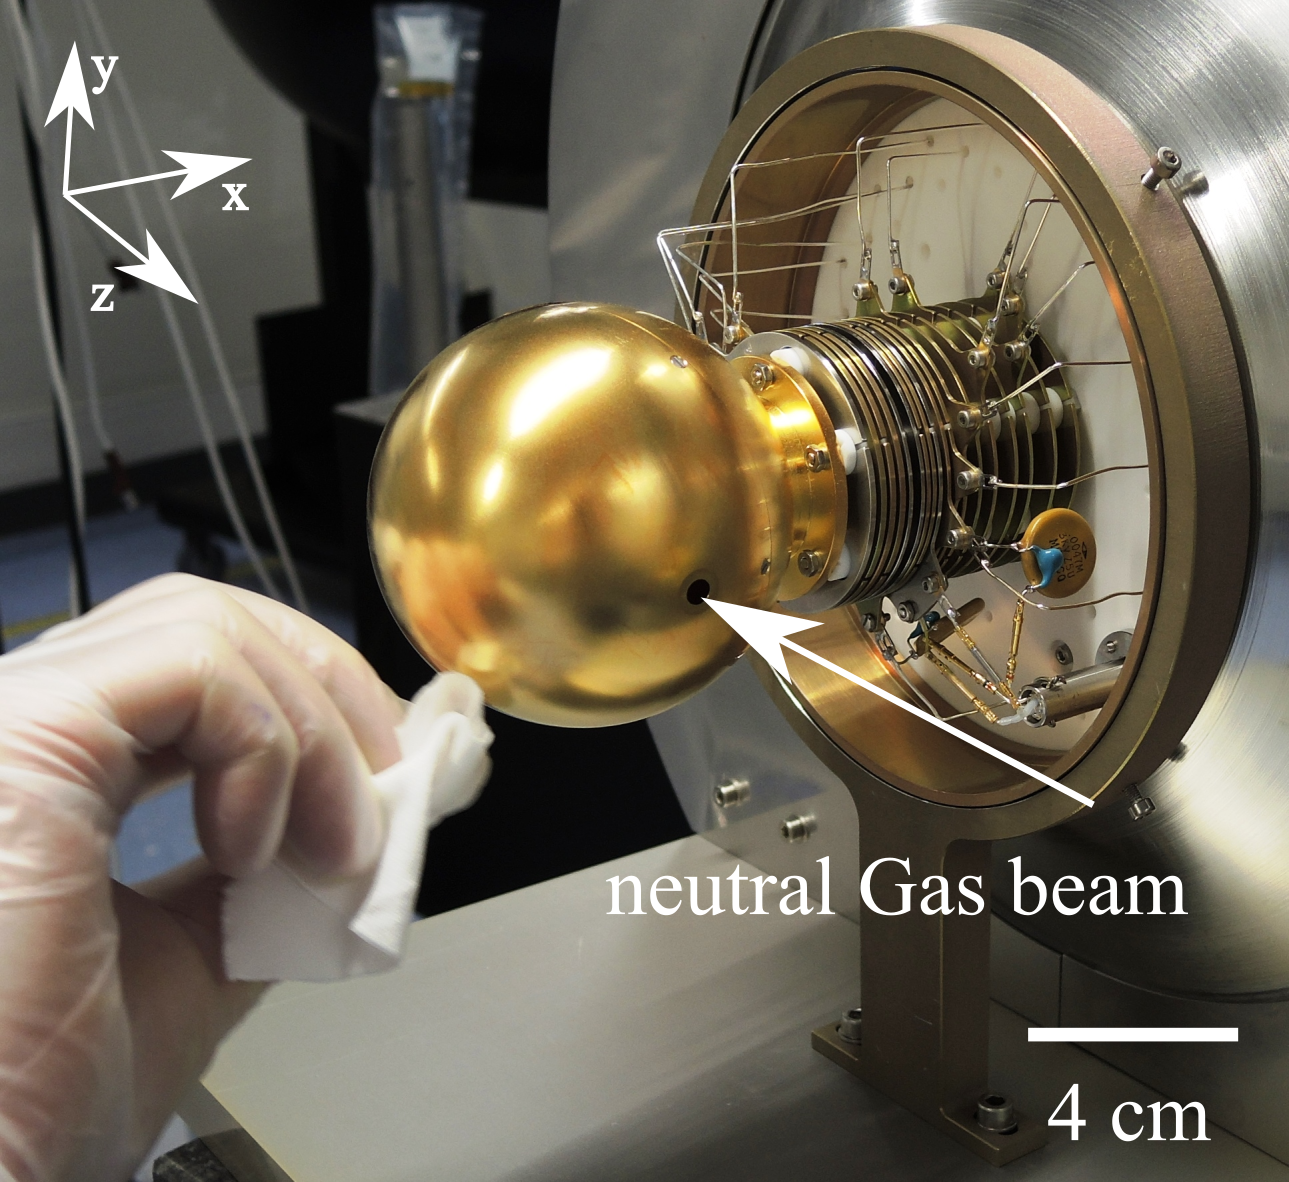
\includegraphics[width = 0.8\textwidth]{Setup/FlightAnte.png}
		\end{subfigure}
		\caption{Left: Prototype antechamber. Right: Flight-like antechamber.}
		\label{fig:SetupAntecham}
	\end{figure}
	\begin{figure}[h] % IS Proto
		\centering
		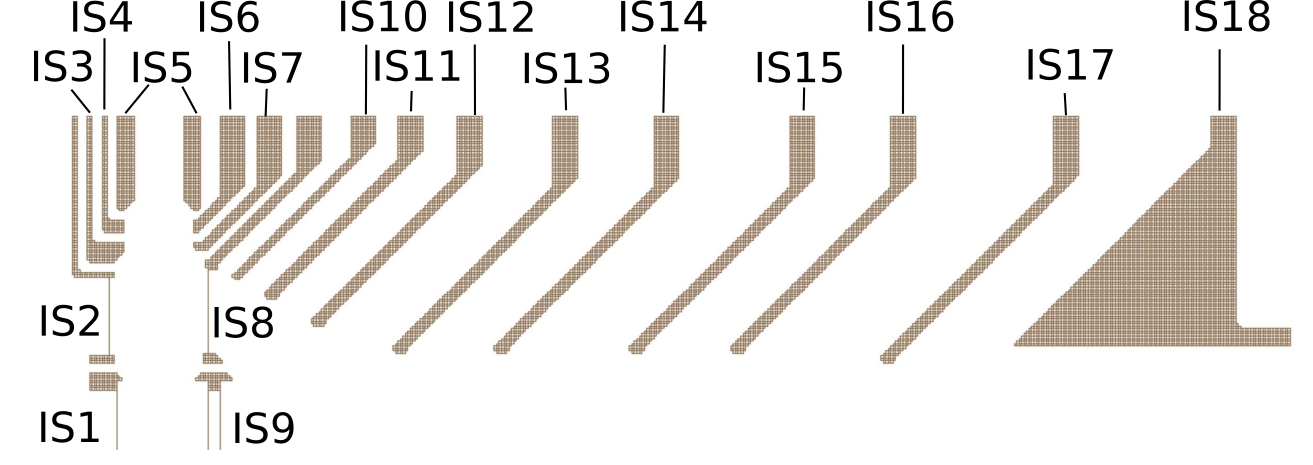
\includegraphics[width= 0.7\textwidth]{Setup/Proto_IS_sim.png}
		\caption{SIMION Model of the Ion-Source of the NIM Prototype \cite{Diss_Meyer}.}
		\label{fig:SetupProtoISSim}
	\end{figure}
	\begin{figure}[h] % IS PFM
		\centering
		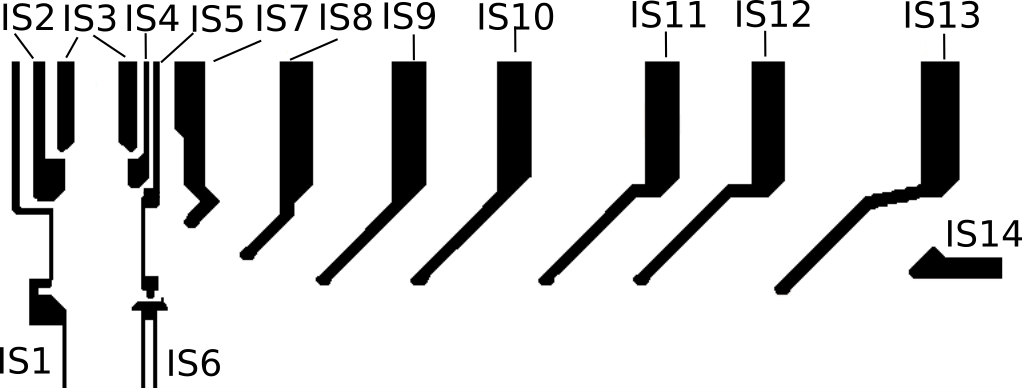
\includegraphics[width=0.7\textwidth]{Setup/ISFlight_bearb.png}
		\caption{SIMION Model of the Ion-Source of the NIM ProtoFlight Model.}
		\label{fig:SetupPFMISSim}
	\end{figure}
	\begin{figure}[h!] % Filament blocs
		\begin{subfigure}{0.5\textwidth}
			\centering
			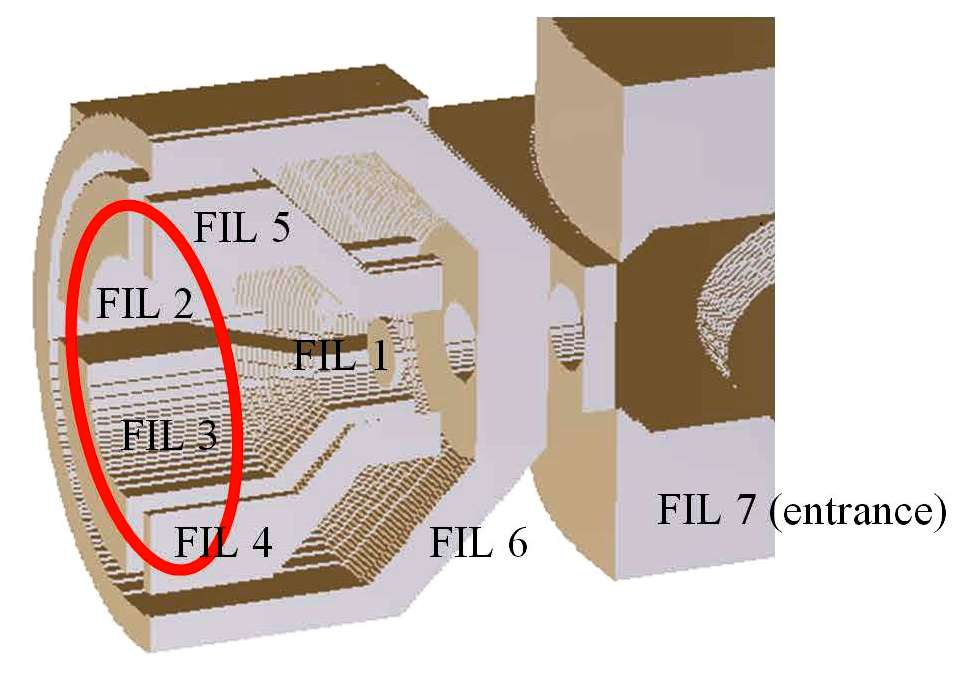
\includegraphics[width =0.85\textwidth]{Setup/Proto_FilEl_sim.jpg}
		\end{subfigure}
		\begin{subfigure}{0.5\textwidth}
			\centering
			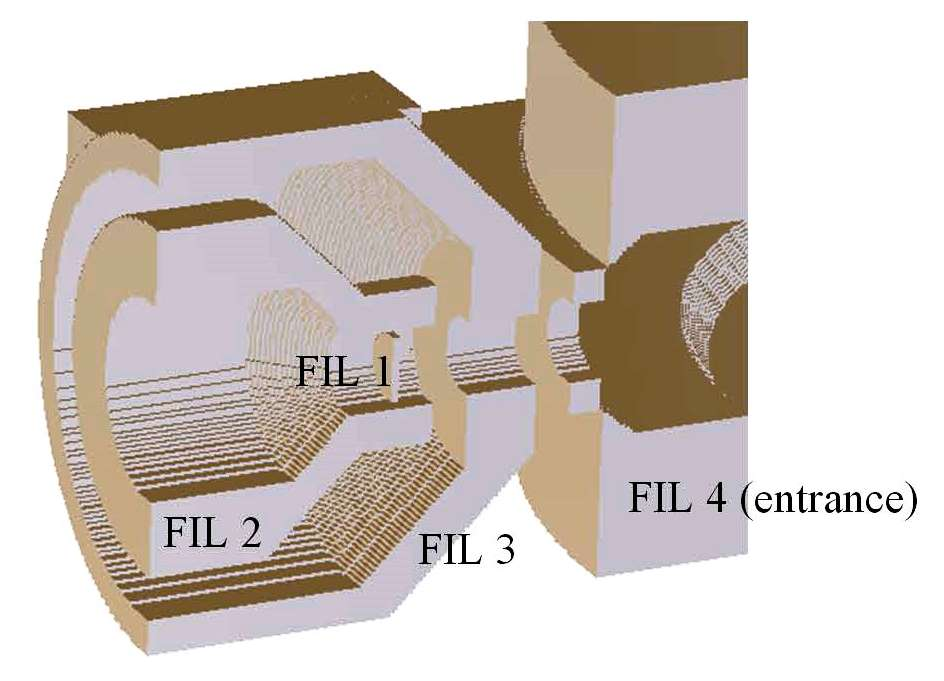
\includegraphics[width = 0.85\textwidth]{Setup/PFM_FilEl_sim.jpg}
		\end{subfigure}
		\caption{Left: Prototype filament housing. Right: PFM filament housing.}
		\label{fig:SetupFilElSim}
	\end{figure}
	This chapter compares the NIM prototype (Fig.~\ref{fig:SetupProto}) with the NIM ProtoFlight Model (PFM) (Fig.~\ref{fig:SetupPFM}) from the mechanical point of view. It shows the key differences between the two models. Special focus lay hereby on the design of the detector because there were made some major design improvements.\\
	Fig.~\ref{fig:SetupAntecham}~left shows the prototype antechamber and right the PFM antechamber. To improve the performance of the antechamber, the flight antechamber was made twice as big as the old one of the prototype. In addition, it has two entrance holes at $\pm$30° relative to the x-axis of the instrument to be able to measure gas coming from both directions of the instrument (see Chap~\ref{subsubsec:Calfly}). The main inflow direction of the neutral particle beam generated by the CASYMIR test facility is 90° \cite{CASYMIR_Graf2004}. Therefore, a second flight-like test antechamber was made which has the second entrance hole at position 90° to be able to test the flight antechamber. The antechambers consists of two parts which are hold together with screws. Tests revealed that two of the mounting screws generate signal artefacts \cite{Meyer_2017_ante}. Therefore, the outer surface of the antechamber was redesigned (see also Chap.~\ref{subsec:ExpAnteCham}).\\
	Fig.~\ref{fig:SetupProtoISSim} shows the SIMION model of the Prototype ion-source, Fig.~\ref{fig:SetupPFMISSim} shows the ion-source of the PFM and Fig.~\ref{fig:SetupFilElSim} shows the filament housing of the Prototype (left) and of the PFM (right). The PFM ion-source has seven electrodes less then the prototype to simplify the source and the flight electronics. Manly LV electrodes were taken together such as IS1\& 2, IS3 \& 4 and IS6 \& 7. IS10 was removed and IS11 was shifted towards the ionisation region. In the filament housing the electron repelling electrodes Fil2--5 were taken together to one single electrode Fil2. The electron repelling electrode in the prototype was split into four parts to compensate with the electric fields for a bad alignment of the filament. For the PFM, the mounting of the filament holder was improved and therefore these four electrodes could be taken together to one single electrode.\\
	Fig.\ref{fig:SetupProtoReflSim} shows a schematics of the ion-mirror. The prototype ion-mirror consists of 14 ring-electrodes (R2--R15). R1 is the drift tube. Between the electrodes R4--R15 are resistors to connect the electrodes with each other to generate a linear voltage gradient when a voltage is applied at electrodes R4 and R15. In addition, a voltage can be applied on electrode R8 allowing additional focusing of the ions in the ion-mirror. The flight ion-mirror consists of a ceramic tube with two resistance spirals on its inner walls replacing electrodes R5--R7 and R9--R14. From the electrical point of view, the two ion-mirrors behave the same.\\
	\begin{figure}[H] % ion mirror
		\centering
		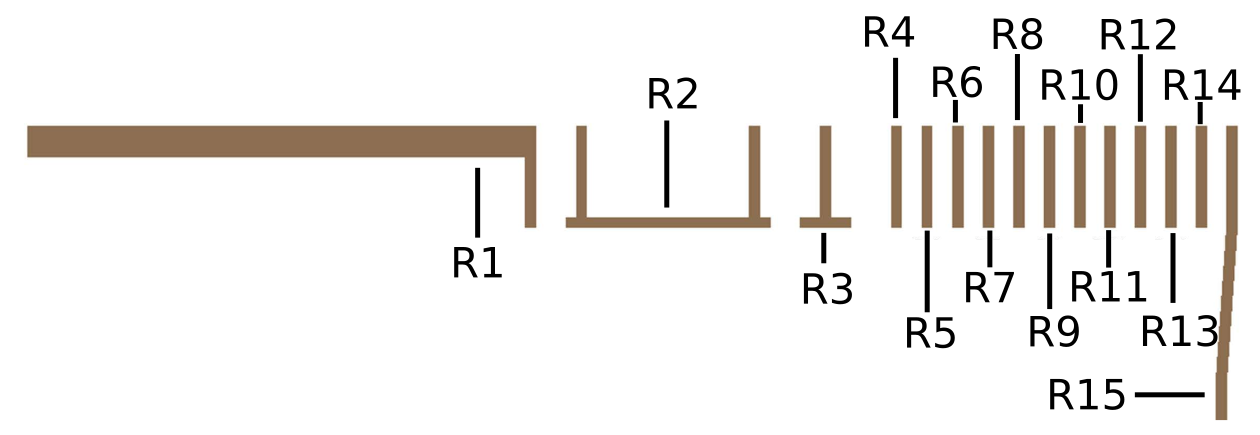
\includegraphics[width=0.9\textwidth]{Setup/Prototype_Reflectron_sim.png}
		\caption{SIMION Model of the ion-mirror of the NIM Prototype \cite{Diss_Meyer}.}
		\label{fig:SetupProtoReflSim}
	\end{figure}
	% Detector Figs.	
	\begin{figure}[H] % Photograph of the Prototype an Flight detector.
		\begin{subfigure}{0.5\textwidth}
			\centering
			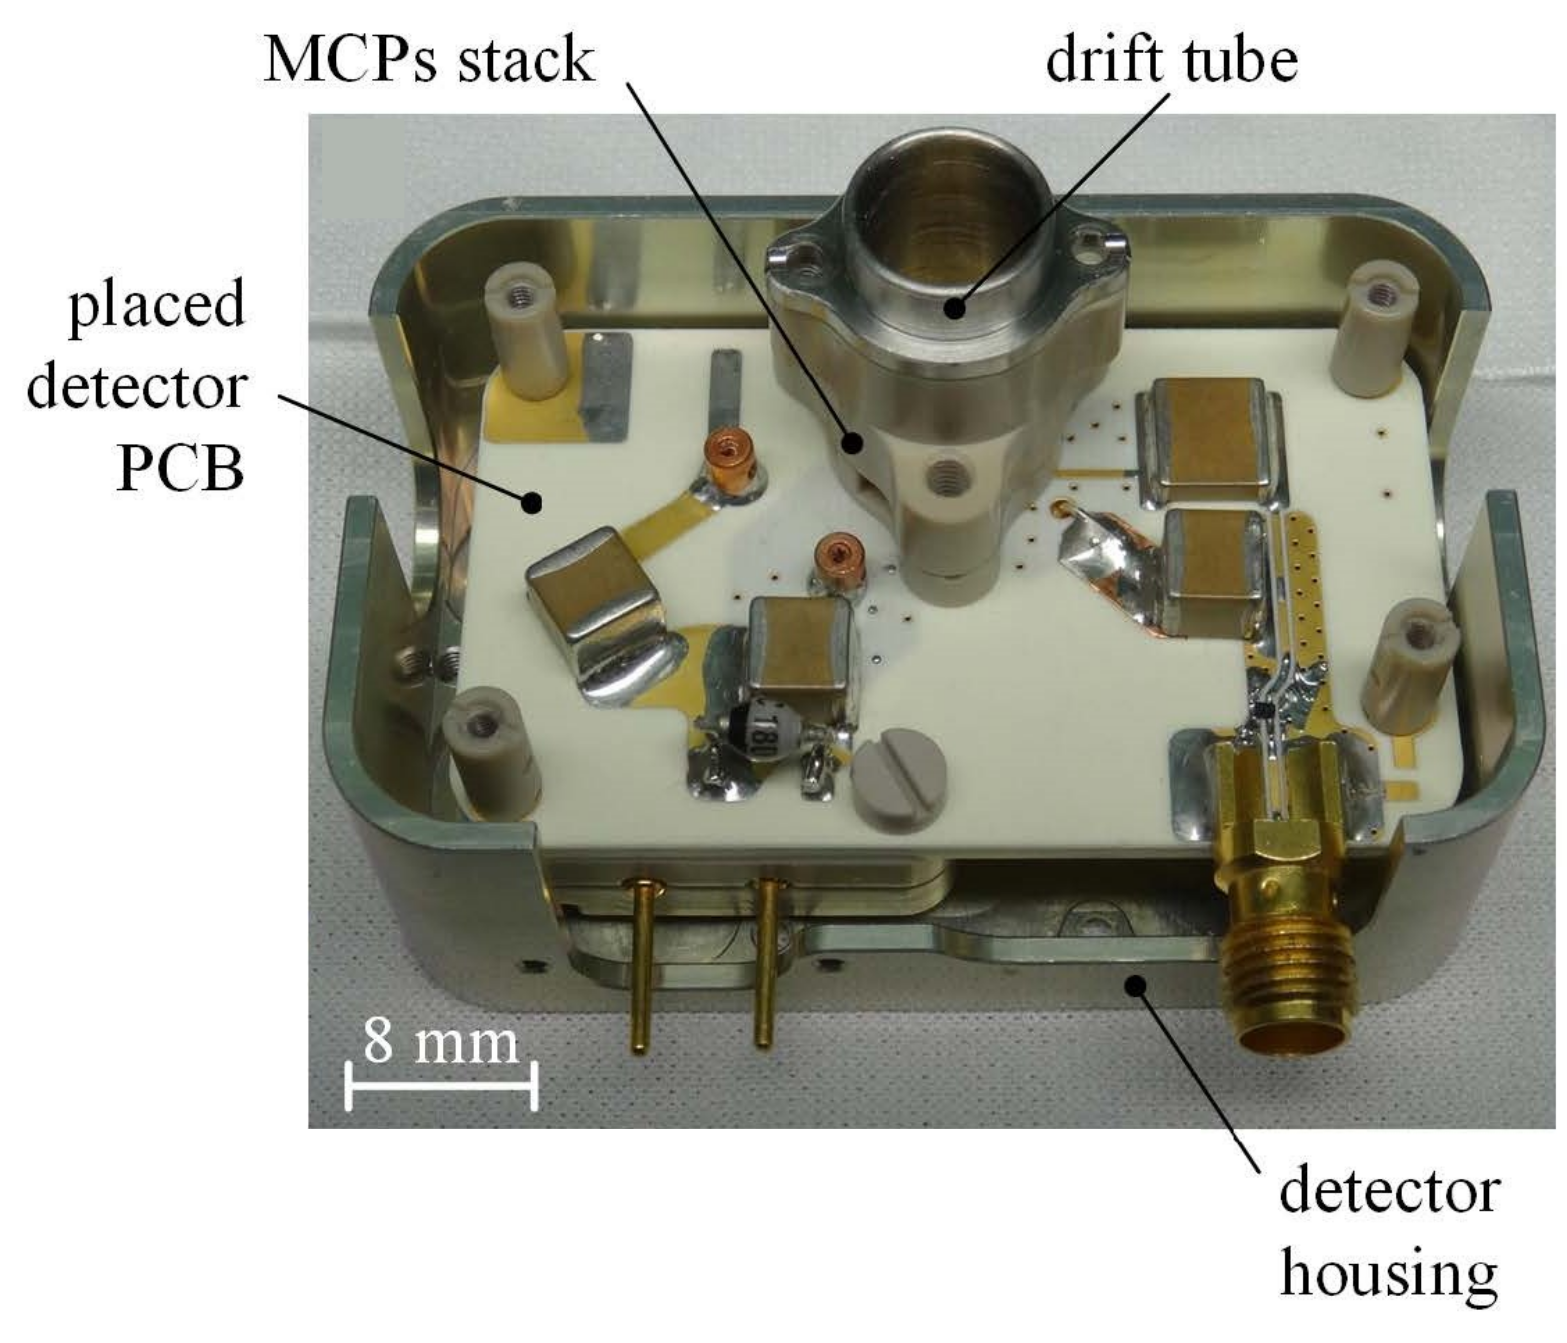
\includegraphics[width=\textwidth]{Setup/Prototype_Detector.png}
		\end{subfigure}
		\begin{subfigure}{0.5\textwidth}
			\centering
			\includegraphics[width=.9\textwidth]{Setup/Flight_Detector.png}
		\end{subfigure}
		\caption{Left: NIM Prototype detector \cite{Diss_Meyer}. Right: NIM Flight detector without its radiation shield.}
		\label{fig:DetPhotos}
	\end{figure}
	\begin{figure}[h] % Schematics of the 2 detector designs.
		\centering
		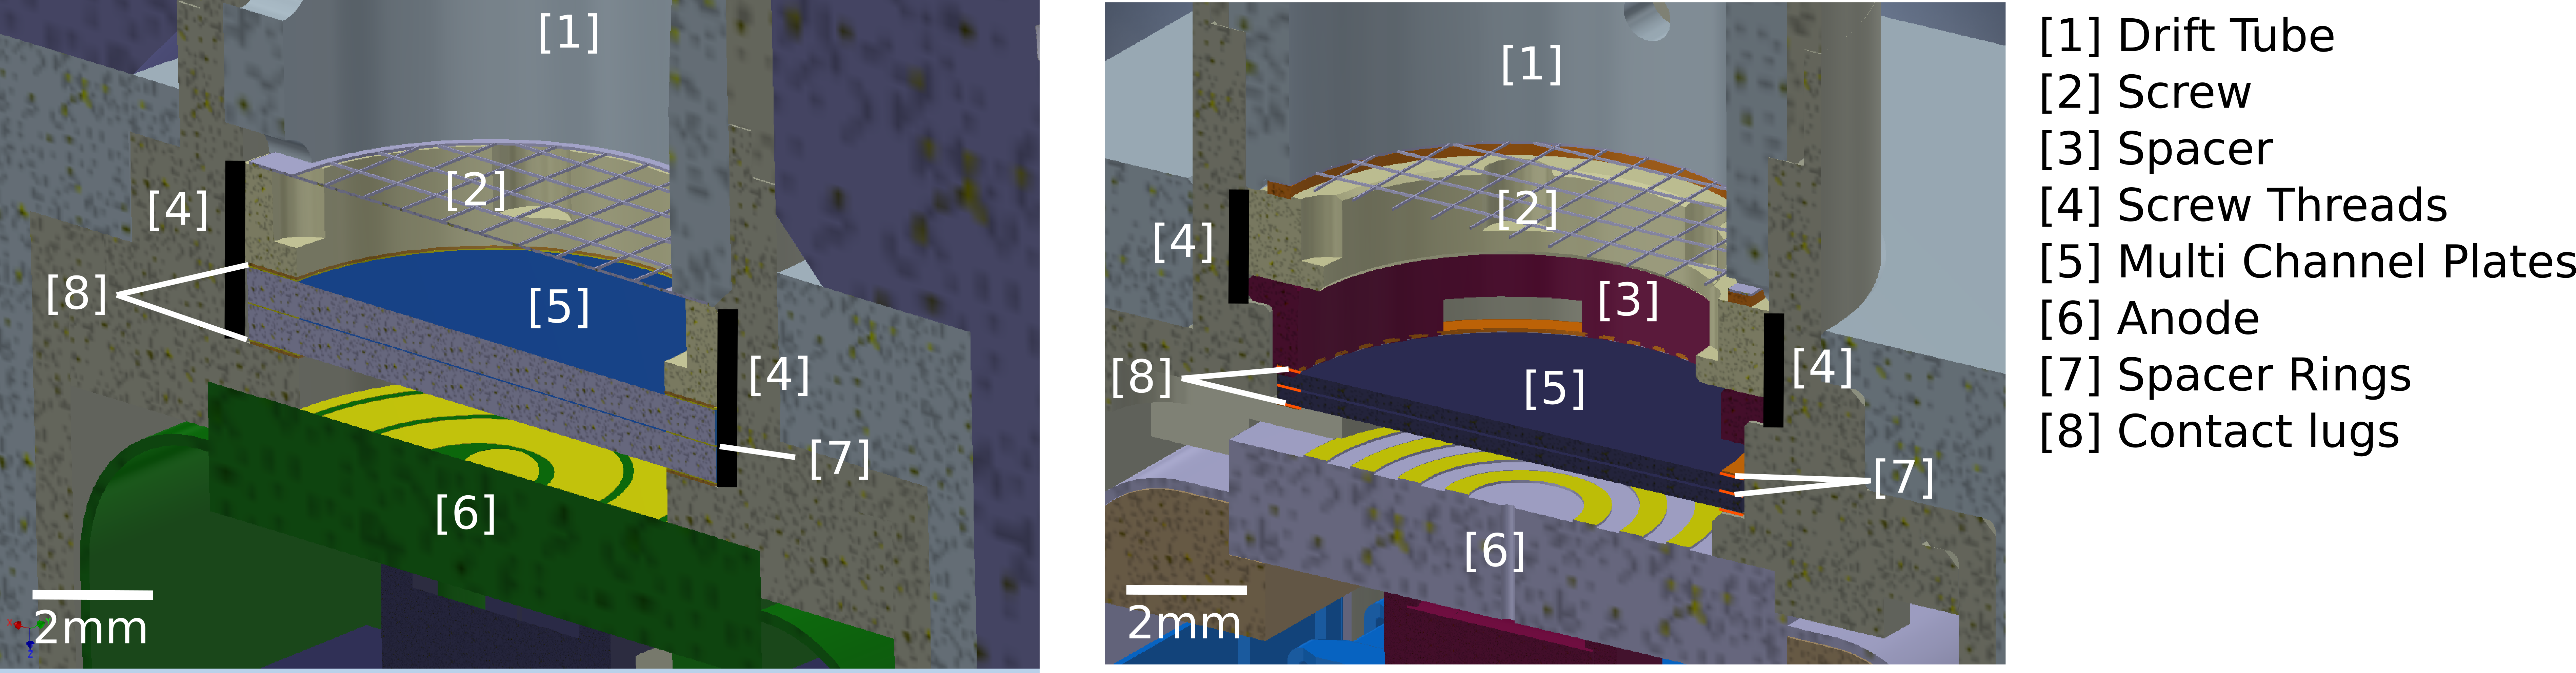
\includegraphics[width= \textwidth]{Setup/PFMDetectors.png}
		\caption{Schematics of the PFM detector housings. Left: preliminary design. Right: final flight design.}
		\label{fig:FlightDetSchemata}
	\end{figure}
	\begin{figure}[h] % Circuit diagram
		\centering
		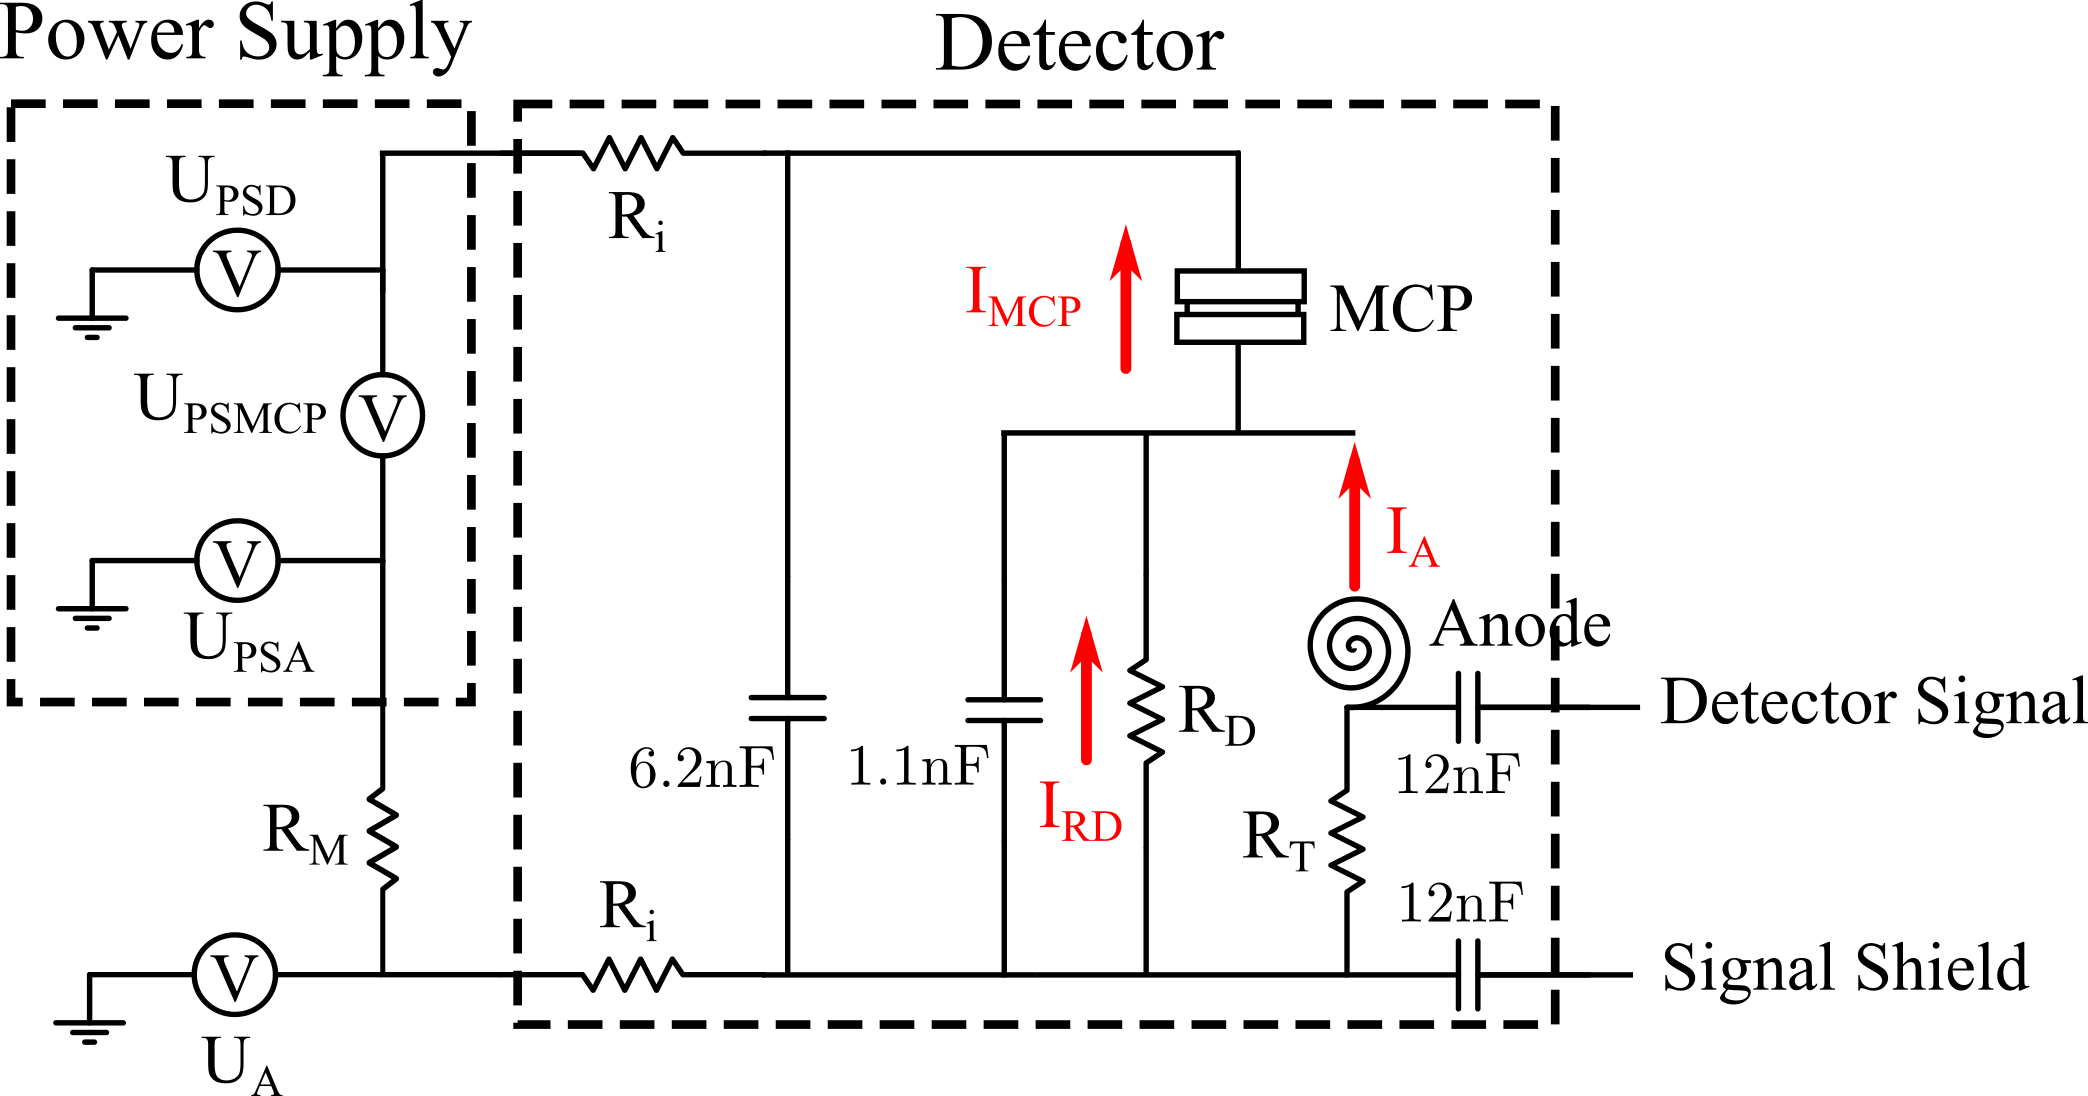
\includegraphics[width = .8\textwidth]{Bilder/Detector_elec_schema.png}
		\caption{Electrical schematics of the NIM flight detector with laboratory electronics attached.}
		\label{fig:FlighElecSchema}
	\end{figure}
	% free play = technisch Spiel. Put it in during proofreading.
	The NIM Prototype detector has a rigid Printed Circuit Board (PCB) on which the electrical components and the drift tube with the MCP stack are mounted (Fig.~\ref{fig:DetPhotos}~left). Due to Jupiter's strong radiation field, the detector has to be shielded to reduce the noise level induced by the strong radiation and to increase the detector's lifetime. To minimized the required shielding mass, the flight detector has to be very compact. This was achieved by using a flex PCB to fold the detector into a peek housing (Fig.~\ref{fig:DetPhotos}~right). Fig.~\ref{fig:FlightDetSchemata}~left shows the schema of a preliminary design of the peek housing containing the MCPs. The MCPs lay on a ledge 1~mm above the anode. A diode generates a voltage between the MCP backside and the anode to accelerate the electrons from the MCP backside towards the anode (see electrical schema Fig,\,\ref{fig:FlighElecSchema}). There are two contact lugs on top and at the bottom of the MCP stack to apply a voltage over the MCPs. The MCPs are fixed with a peek screw within the housing. In the old design, the screw threads were milled down to the ledge. When the MCPs were mounted, they often canted in the threads. In addition, it was not possible to determine, how much the screw had to be tightened. When the screw was tighten too much, the MCPs broke as they consist of lead glass and are therefore very fragile. When the screw was too loose, the two contact lugs had no reliable contact to the MCPs. When applying a high voltage over the whole MCP stack, the gaps between the contact lugs and the MCPs act as an additional resistors over which the voltage builds up resulting in a discharge between the electrodes and the MCPs. The discharge can propagate through the whole MCP stack and damages the readout electronics. As a consequence, the screw thread was milled less far and an additional mechanical stop was made to tighten the screw only down to that stop (Fig.\,\ref{fig:FlightDetSchemata}~right). This prevented the MCPs from canting in the screw thread thus it was not milled down to the bottom of the lower ledge and with the mechanical stop, the screw could not be tightened too much to break the MCPs. In addition, a peek space was added between the screw and the MCPs to push down the MCPs uniformly. Due to the tolerances in the manufacturing process of the different parts of the housing, metallic spacer rings are added between the peek spacer and the contact lug of the top MCP to close the resulting gap. The number of added rings varies between each detector because the gap is different for each manufactured housing. With this design, the contact between the MCPs and the contact lugs could be improved but from the electrical point of view its still not a clean electrical contact. To make the system more robust against discharges the Zener diode was exchanged through a resistor ($R_D$ in Fig.~\ref{fig:FlighElecSchema}). The flight electronics sets the voltage $U_{stack}$ between the top MCP and the anode. The MCPs and the diode act as resistors, which are connected in series. Therefore, the potential drop over the MCPs depends on the potential drop over the diode. The voltage drop over a Zener diode is 180~V independent of $U_{stack}$. Therefore, the voltage over the MCPs $U_{MCP}$ is 180~V lower than $U_{stack}$. When having a resistor $R_D$ instead of a diode, the voltage over the MCPs cannot be calculated by just having $U_{stack}$ because the resistance of the MCPs $R_{MCP}$ depends on the voltage $U_{MCP}$ applied over them. It also changes with time due to ageing because the conductive material inside the MCP channels degrades over time. Therefore, the current $I_{MCP}$ flowing through the system has to be known to be able to calculate $U_{MCP}$. The NIM flight electronics is not designed to measure this current because it was designed for a detector with a diode where a current measurement would be unnecessary. A calibration with the laboratory electronics was done to determine the relationship between $U_{stack}$ and $U_{MCP}$ (Chap.~\ref{chapExp:Det}).\\
	In the following section, $U_{MCP}$ is derived as a function of the different voltages known when measuring with laboratory electronics. Fig.~\ref{fig:FlighElecSchema} shows the circuit diagram of the detector when operated with laboratory electronics and Table~\ref{tab:ElecSchemaVariableList} summarizes the used variables. The current flowing through the MCPs $I_{MCP}$ is measured with the resistor $R_M$:
	\begin{equation}
		I_{MCP} = \frac{U_{RM}}{R_{M}}
	\end{equation}
	With $U_{RM}$ the voltage over the resistor $R_{M}$ which is:
	\begin{align}
		U_{RM} &= U_{PSA} - U_{A}\\
			   &= U_{PSMCP} + U_{PSD} - U_A
	\end{align}
	With $U_{PSA}$ the power supply output voltage for the anode, $U_{A}$ the voltage applied on the detector anode, $U_{PSD}$ the power supply output voltage applied at the top contact lug of the MCP stack and $U_{PSMCP}$ the voltage difference between the two power supply outputs. $U_{PSMCP}$ is:
	\begin{equation}
		U_{PSMCP} = U_{RM} + 2\cdot U_{Ri} + U_{RD} + U_{MCP}
		\label{eq:UpsmcpTot}
	\end{equation}
	With $U_{Ri}$ the voltage over the input resistors $R_i$, which are there to damp noise coupled into the detector circuit from the power supply:
	\begin{equation}
		U_{Ri} = I_{MCP}\cdot R_i
	\end{equation} 
	$U_{RD}$ is the voltage over the resistor $R_D$ replacing the former diode. The current $I_A$ induced when an ion generates an electron avalanche, is very low compared to the current $I_{RD}$. Therefore, $I_{MCP} = I_{RD}$ and:
	\begin{equation}
		U_{RD} = I_{MCP}\cdot R_D
	\end{equation}
	Solving Eq.~\eqref{eq:UpsmcpTot} to $U_{MCP}$ and inserting the different voltages results in:
	\begin{align}
		U_{MCP} =& U_{PSMCP} - U_{RM} - 2\cdot U_{Ri} - U_{RD}\\
				=& U_{PSMCP} - U_{PSMCP} + U_{PSD} - U_A - 2\cdot I_{MCP} R_i - I_{MCP} R_D\\
				=& (U_A - U_{PSD})\cdot(1 + \frac{2R_i + R_D}{R_M}) - U_{PSMCP}\frac{2R_i + R_D}{R_M}
	\end{align}	
	
	\begin{table}[h]
		\begin{center}
		\begin{tabular}{|m{1.5cm}|m{5.4cm}|m{1.5cm}|m{5.4cm}|}
			\hline
			R\textsubscript{D}& Resistor replacing the former diode & U\textsubscript{A}& Voltage on the detector anode \\
			R\textsubscript{i} & Detector input resistor & U\textsubscript{MCP}& Voltage over the MCPs \\
			R\textsubscript{M}& Resistor used to determine I\textsubscript{MCP} &U\textsubscript{PSA} & Anode voltage output of power supply \\
			R\textsubscript{MCP}& MCP resistance & U\textsubscript{PSD} & Drift voltage output of power supply \\
			R\textsubscript{T} & 50\,$\Omega$ termination & U\textsubscript{PSMCP} & Voltage difference  between U\textsubscript{PSA} and U\textsubscript{PSD} \\
			I\textsubscript{A} & Current induced in the MCPs when an ion hits the MCPs & U\textsubscript{RD}& Voltage over R\textsubscript{D} \\
			I\textsubscript{ion} & Ion current hitting the MCPs & U\textsubscript{Ri}& Voltage over R\textsubscript{i} \\
			I\textsubscript{MCP} & Current flowing through the MCPs &U\textsubscript{RM}& Voltage over test resistor R\textsubscript{M}\\
			I\textsubscript{RD} & Current flowing through R\textsubscript{D} &&\\
			\hline
		\end{tabular}
		\end{center}
		\caption{List of the variables used in the schematics of the flight detector Fig.~\ref{fig:FlighElecSchema} when the detector is operated with laboratory electronics.}
		\label{tab:ElecSchemaVariableList}
	\end{table}
	\begin{figure}[h!]
		\centering
		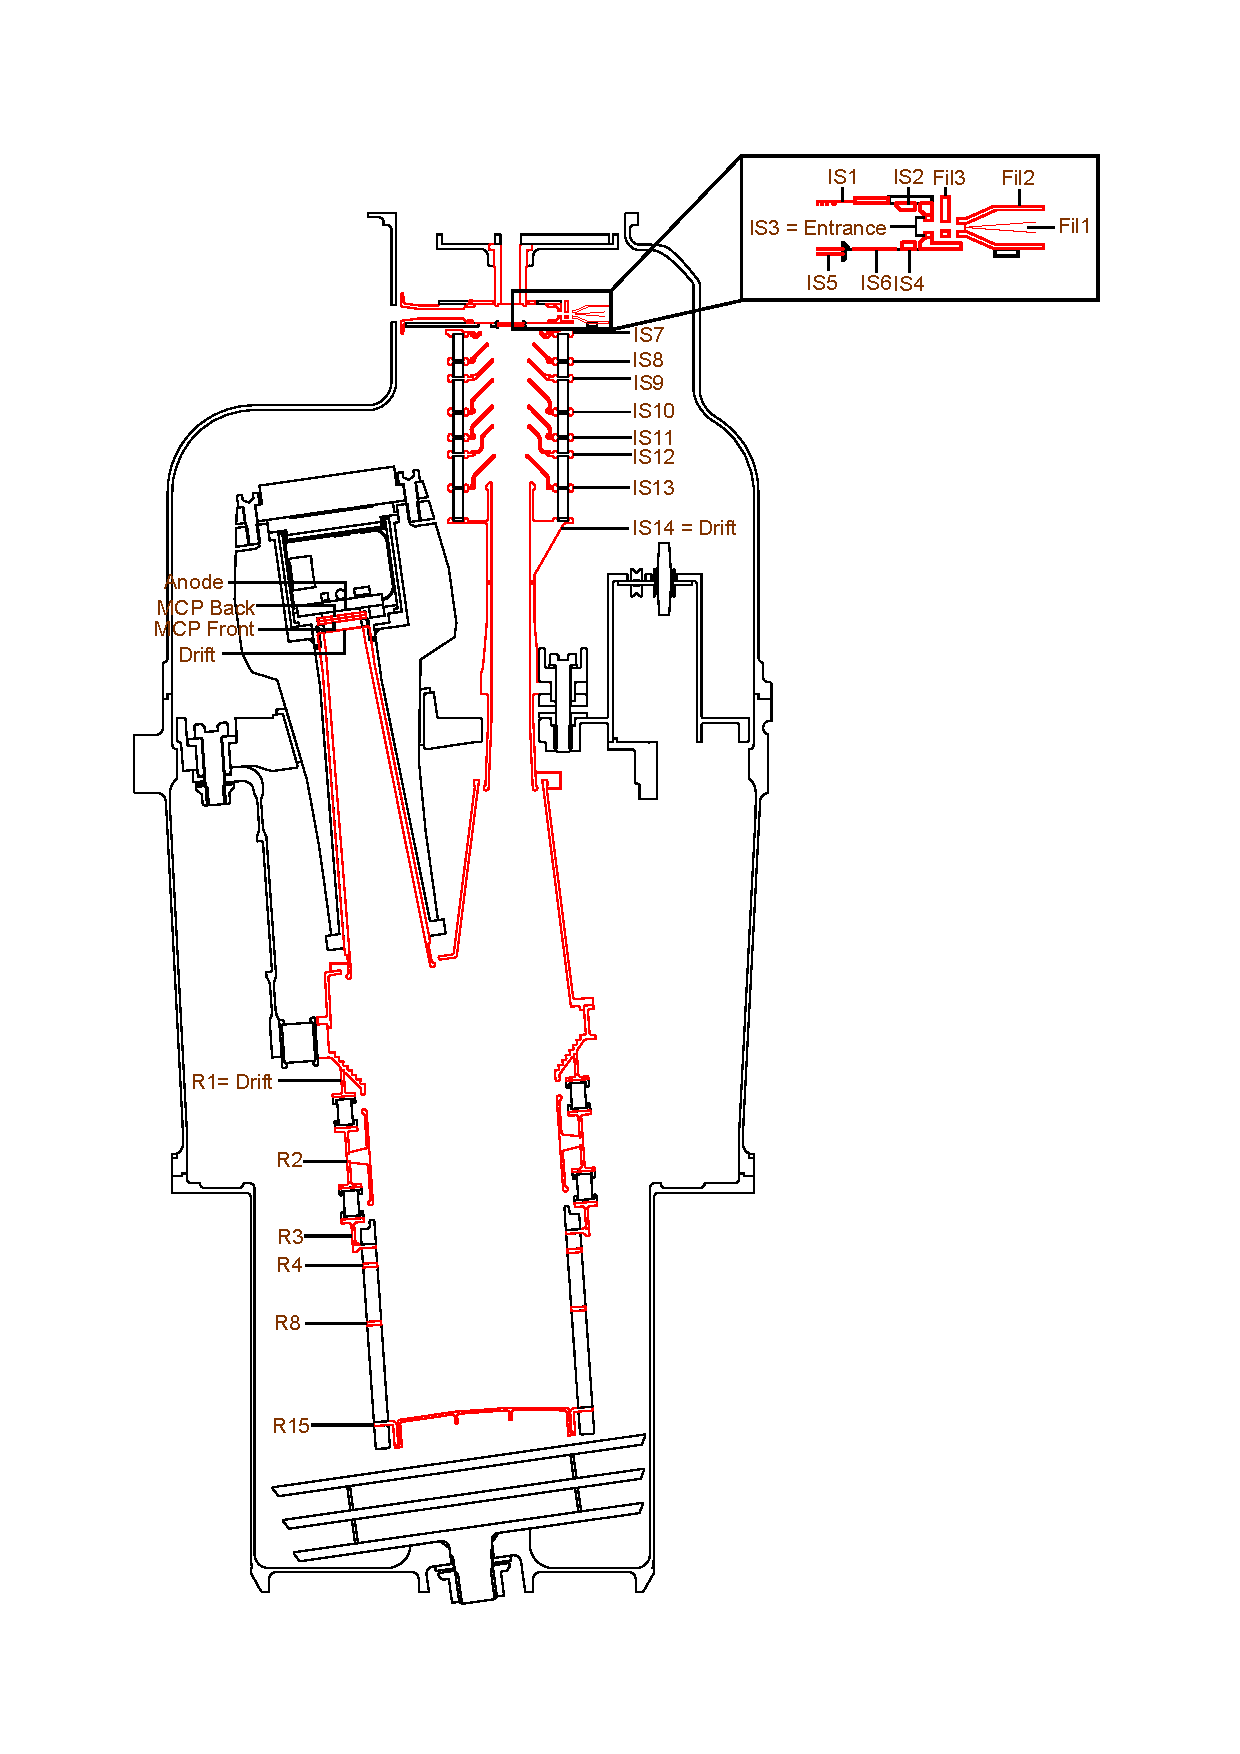
\includegraphics[width= 0.95\textwidth]{Setup/NIM_schema.pdf}
		\caption{Schematics of the NIM flight design with all electrodes marked in red.}
		\label{fig:MINPFMTot}
	\end{figure}
	\begin{comment}
	% Pumpstand nr.~2 was used to perform stand-alone tests with the different NIM detectors. The test setup consists of a vacuum chamber, a HV power supply, an oscilloscope, a computer to remote control the oscilloscope and a HV meter (Fig.~\ref{fig:Pumpstand2}).		
	
	\begin{figure}[h]
	\begin{subfigure}{.5\textwidth}
	\centering
	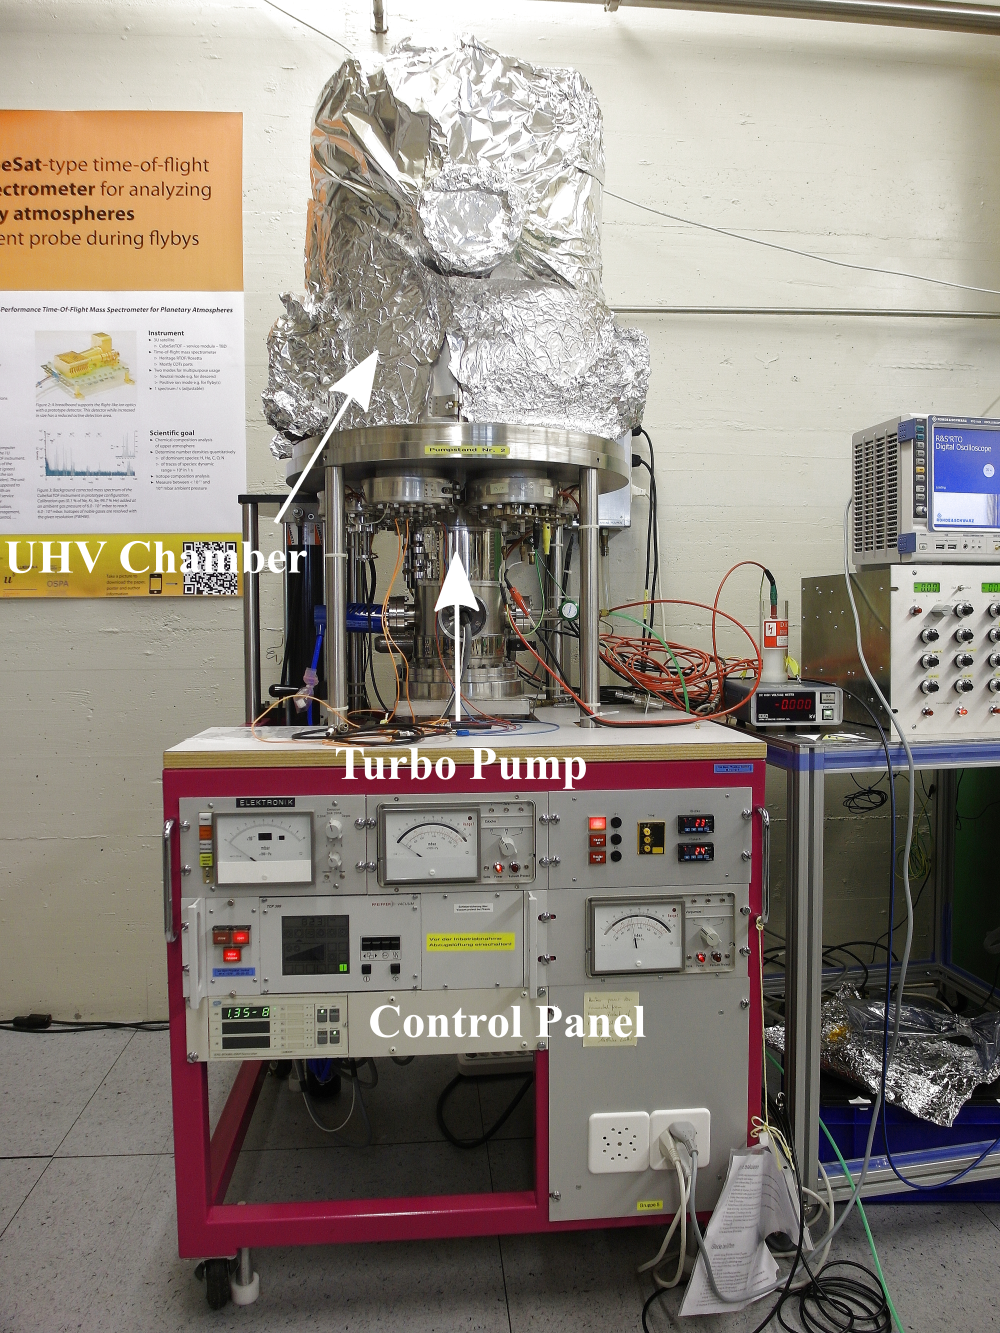
\includegraphics[width=0.8\textwidth]{Bilder/Galerie_Setup/Pumpstand2_midres.png}
	\end{subfigure}
	\begin{subfigure}{.5\textwidth}
	\centering
	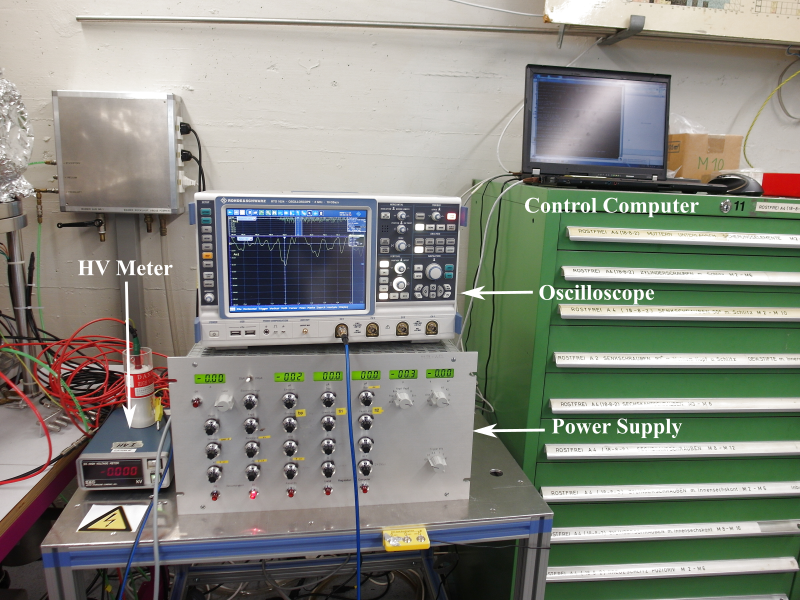
\includegraphics[width=\textwidth]{Bilder/Galerie_Setup/Pumpstand_PSOszi.png}
	\end{subfigure}
	\caption{Left: Pumpstand nr. 2. Right: Power supply, oscilloscope and control computer for the stand-alone tests of the detector. The signal on the oscilloscope is a noise signal.}
	\label{fig:Pumpstand2}
	\end{figure}
	\end{comment}



	% NIM Instrument description overview. Startconfiguration.
	\clearpage
	\newpage
	\thispagestyle{empty}
	\null
	\newpage
	% !TEX root = arbeit.tex
\section{Experiments} \label{sec:Exp}
	The tests described in this chapter include tests of the different components of the NIM instrument such as laboratory tests of the flight antechamber tested on the Prototype or the flight ion-mirror. The part of Chapter \ref{sec:Exp} includes manly test with the prototype, later on tests with the PFM and follow.

% In zeitlicher Reihenfolgen auflisten, damit man sieht, zu welchem Zeitpunkt man mit welchen Teilen gearbeitet hat.
% In this section, all the different test (lab and simulations) are listed. As far as possible in their chronolocial order because between some lab tests there were simulations to improve the instrument before testing the redesigned instrument.

% Fügt ein PDF ein, nummeriert nach dem PDF normal weiter.
%\includepdf[pages=-]{Report_Thermofoil_UV_Masterarbeit.pdf}

% Section über Detector? haben wir ja nicht wirklich etwas gemacht. Diode durch 2 Widerstände ersetzt. -> Spannungsfestigkeit. Verlauf der Überschläge. Unterschiedliche Skizzen.

	In this section, the different tests are described to develop the NIM instrument. Different parts of the instrument were tested to improve the instrument.
%-----------------------------------------------------------------------------------
	\subsection{Ion-Mirror}
	% Test of subcomponents.
	The NIM prototype reflectron was exchanged through the flight like reflectron, which was tested. The NIM prototype reflectron consisted of 12 ring electrodes connected with each other with resistors in between them. On the first, 5th and 12th electrode, a voltage can be applied. With the different resistors, a linear voltage gradient in the reflectron is generated.\\ % Noch besser formulieren.
	The flight reflectron consists of a ceramic tube with two resistance spirals on its inner walls. There are three electrodes, where the voltage can be applied. The electrodes are connected via resistance spirals with each other. The two reflectrons can be seen in Fig.\,\ref{fig:ExpRefl}. This kind of reflectron was also used in the RTOF mass spectrometer which flied in ROSINA \cite{Diss_Scherer} and the in the NGMS \cite{Diss_Hofer}. \\ % Evt. noch etwas schöner und weiter ausführen. Strahlungsfestigkeit musste getestet werden. Report? Paper? Diss?
	Therefore, the two reflectrons are from the electrical point of view the same.\\ % Oder kommt das erst bei der Auswertung?
	
	\begin{figure}[h]
		\begin{subfigure}{0.5\textwidth}
			\centering
			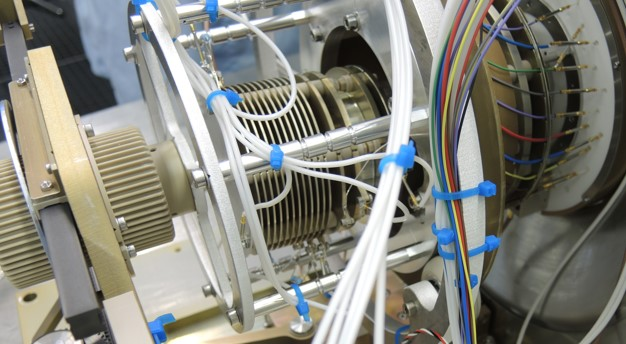
\includegraphics[width = 0.95\textwidth]{Experiments/reflectron_Prototype1.jpg}
		\end{subfigure}
		\begin{subfigure}{0.5\textwidth}
			\centering
			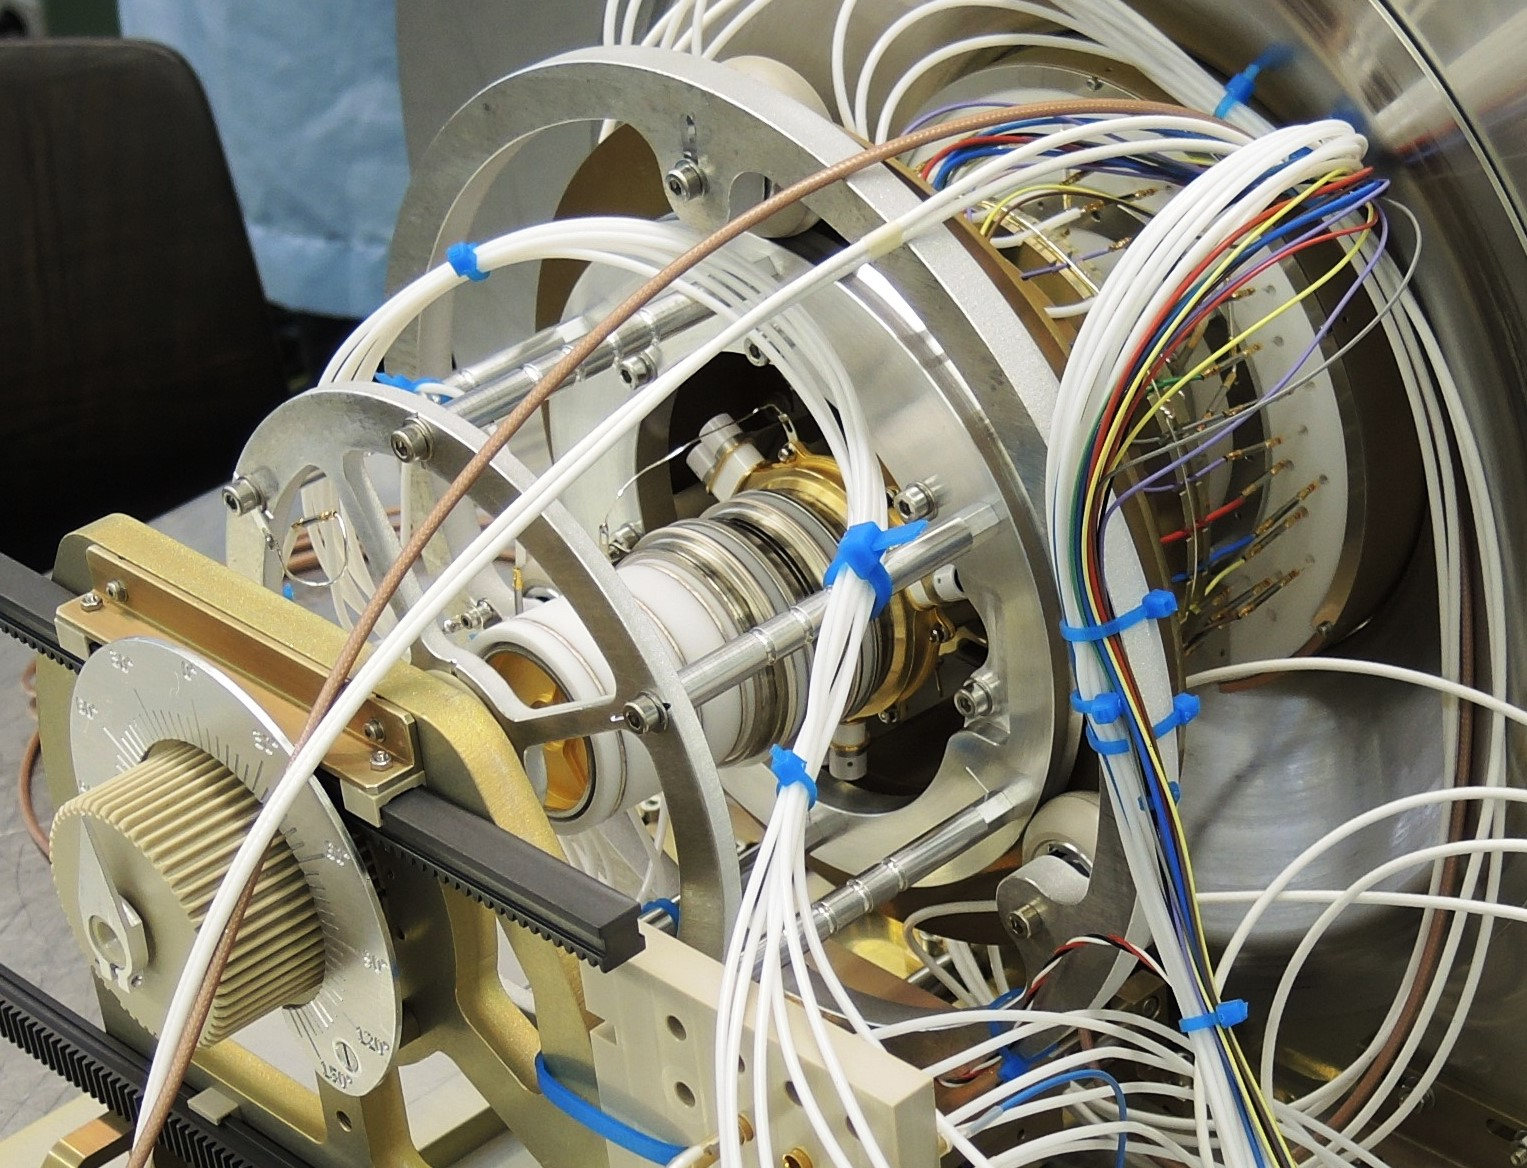
\includegraphics[width = 0.85\textwidth]{Experiments/reflectron_flight.JPG}
		\end{subfigure}
		\caption{Left: Prototype reflectron with ringelectrodes. Right: Flight reflectron}
		\label{fig:ExpRefl}
	\end{figure}

	\subsubsection{Measurement Principle}\label{subsec:ReflecMeasPric}
		% Vortrag Messbedingungen zusammenschreiben
	
	\subsubsection{Discussion}\label{subsec:ReflecDissc}
		% Graphiken neu machen. Achsenskalierung, Spannungssets-Vergleich? Nur sagen, dass sie beinahe identisch sind.
	
	
	% Messbedingungen. Eigenes kurzes Unterkapitel machen
	% Auswertung, eigenes kurzes Unterkapitel

	\begin{comment}
	
	Exchange of the reflectron. Messdaten und Auswertung. Spannungssets vergleichen. Vortrag zusammenschreiben. Plots von dort nehmen und noch etwas besser beschreiben.
	(Plot-Axis, enlarge the exponent of the 10^11 e-/ns)
						
	\end{comment}
	
	
	
	\subsection{Prototype CASYMIR-D/-E}
	% CASYMIR-D? Erst wenn man intensitätsproblem mit ante chamber gelöst hat :/. CASYMIR-E-Kampagne.
	% Kurzfassung?
	
%--------------------------------------------------------------------------------
	\subsection{Simulations}
	
	During development, the mounting of the HV lenses was adapted. Simulations had to be done because as a result of the changed form of the lenses, the voltage set also changed. In this case, the voltage ranges increase by about blabla volts. These new higher ranges challenged the design of the supply electronics because the electronics has a limited amount of space. % Look up the details. Explanation with the electric fields?
	
	%\textcolor{red}{\textbf{Simulations of the adaption of the mounting of the electrodes has to come before the experiments with the PFM although the PFM structure is explained before.}}
	
	% Maybe an other arrangement of the Simulations chaper. See whicht simulations are performed how far any in which order they have to be to be comprehendible.
	
	% Evt. in einem eigenen Kapitel? Schauen, welchen Einfluss es dann jeweis auf die Hardware hatte. -> Elektronik setzt Spannungsranges, beschreiben, dass man da iterieren musste um das optimale Simulationsspannungsset zu finden mit den Grenzen, welche die Elektronik uns für die jeweiligen Elektroden gibt. -> vgl. mit den Messungen vom PFM.
	% Neusimulationen mit neuen Grenzen für die HV. -> die Resultate dieser Simulationen. Als Folgen davon wurden die Grenzen für die HV neu definiert. Schauen, wie man das am besten auseinander nimmt :/.

	% Change of the mounting of the IS lenses -> change in voltages

	% Pulsersimulationen -> Kriterien für Andy für das Pulserdesign. Ab wann wir einen Einbruch in der Massenauflösung haben. (Worddokument wo die einzelnen Bilder zusammengestellt sind?)
	
	% Filament repeller simulation tests. Noch Graphiken einmal einfügen. Die wichtigsten.
	% Um herauszufinden, wie wichtig die Position des Filaments ist.
	
	% Noch besser umschreiben. Die position des filaments entspricht nicht der erwarteten??? Was ist da schief gelaufen??? :(
	
	% Intensitätssimulation Countberechnung:
	% Man generiert 2000 e- auf dem Filament und zeichnet immer nach 1E-5 microsec auf, an welcher Position sich die Teilchen gerade befinden. Die Fkt. 'Plot_optVoltAndPos.m' zählt alle Positionen zusammen, welche sich in dem Zylindervolumen befinden. Die Grundfläche des Zylinders ist das Eintritts-Grid von der antechamber und die Höhe ist die Höhe der Entrance. Im th-Mode befinden sich nur in diesem Volumen neutrale Teilchen.
	\begin{figure}[h]
		\begin{subfigure}{0.53\textwidth}
			\centering
			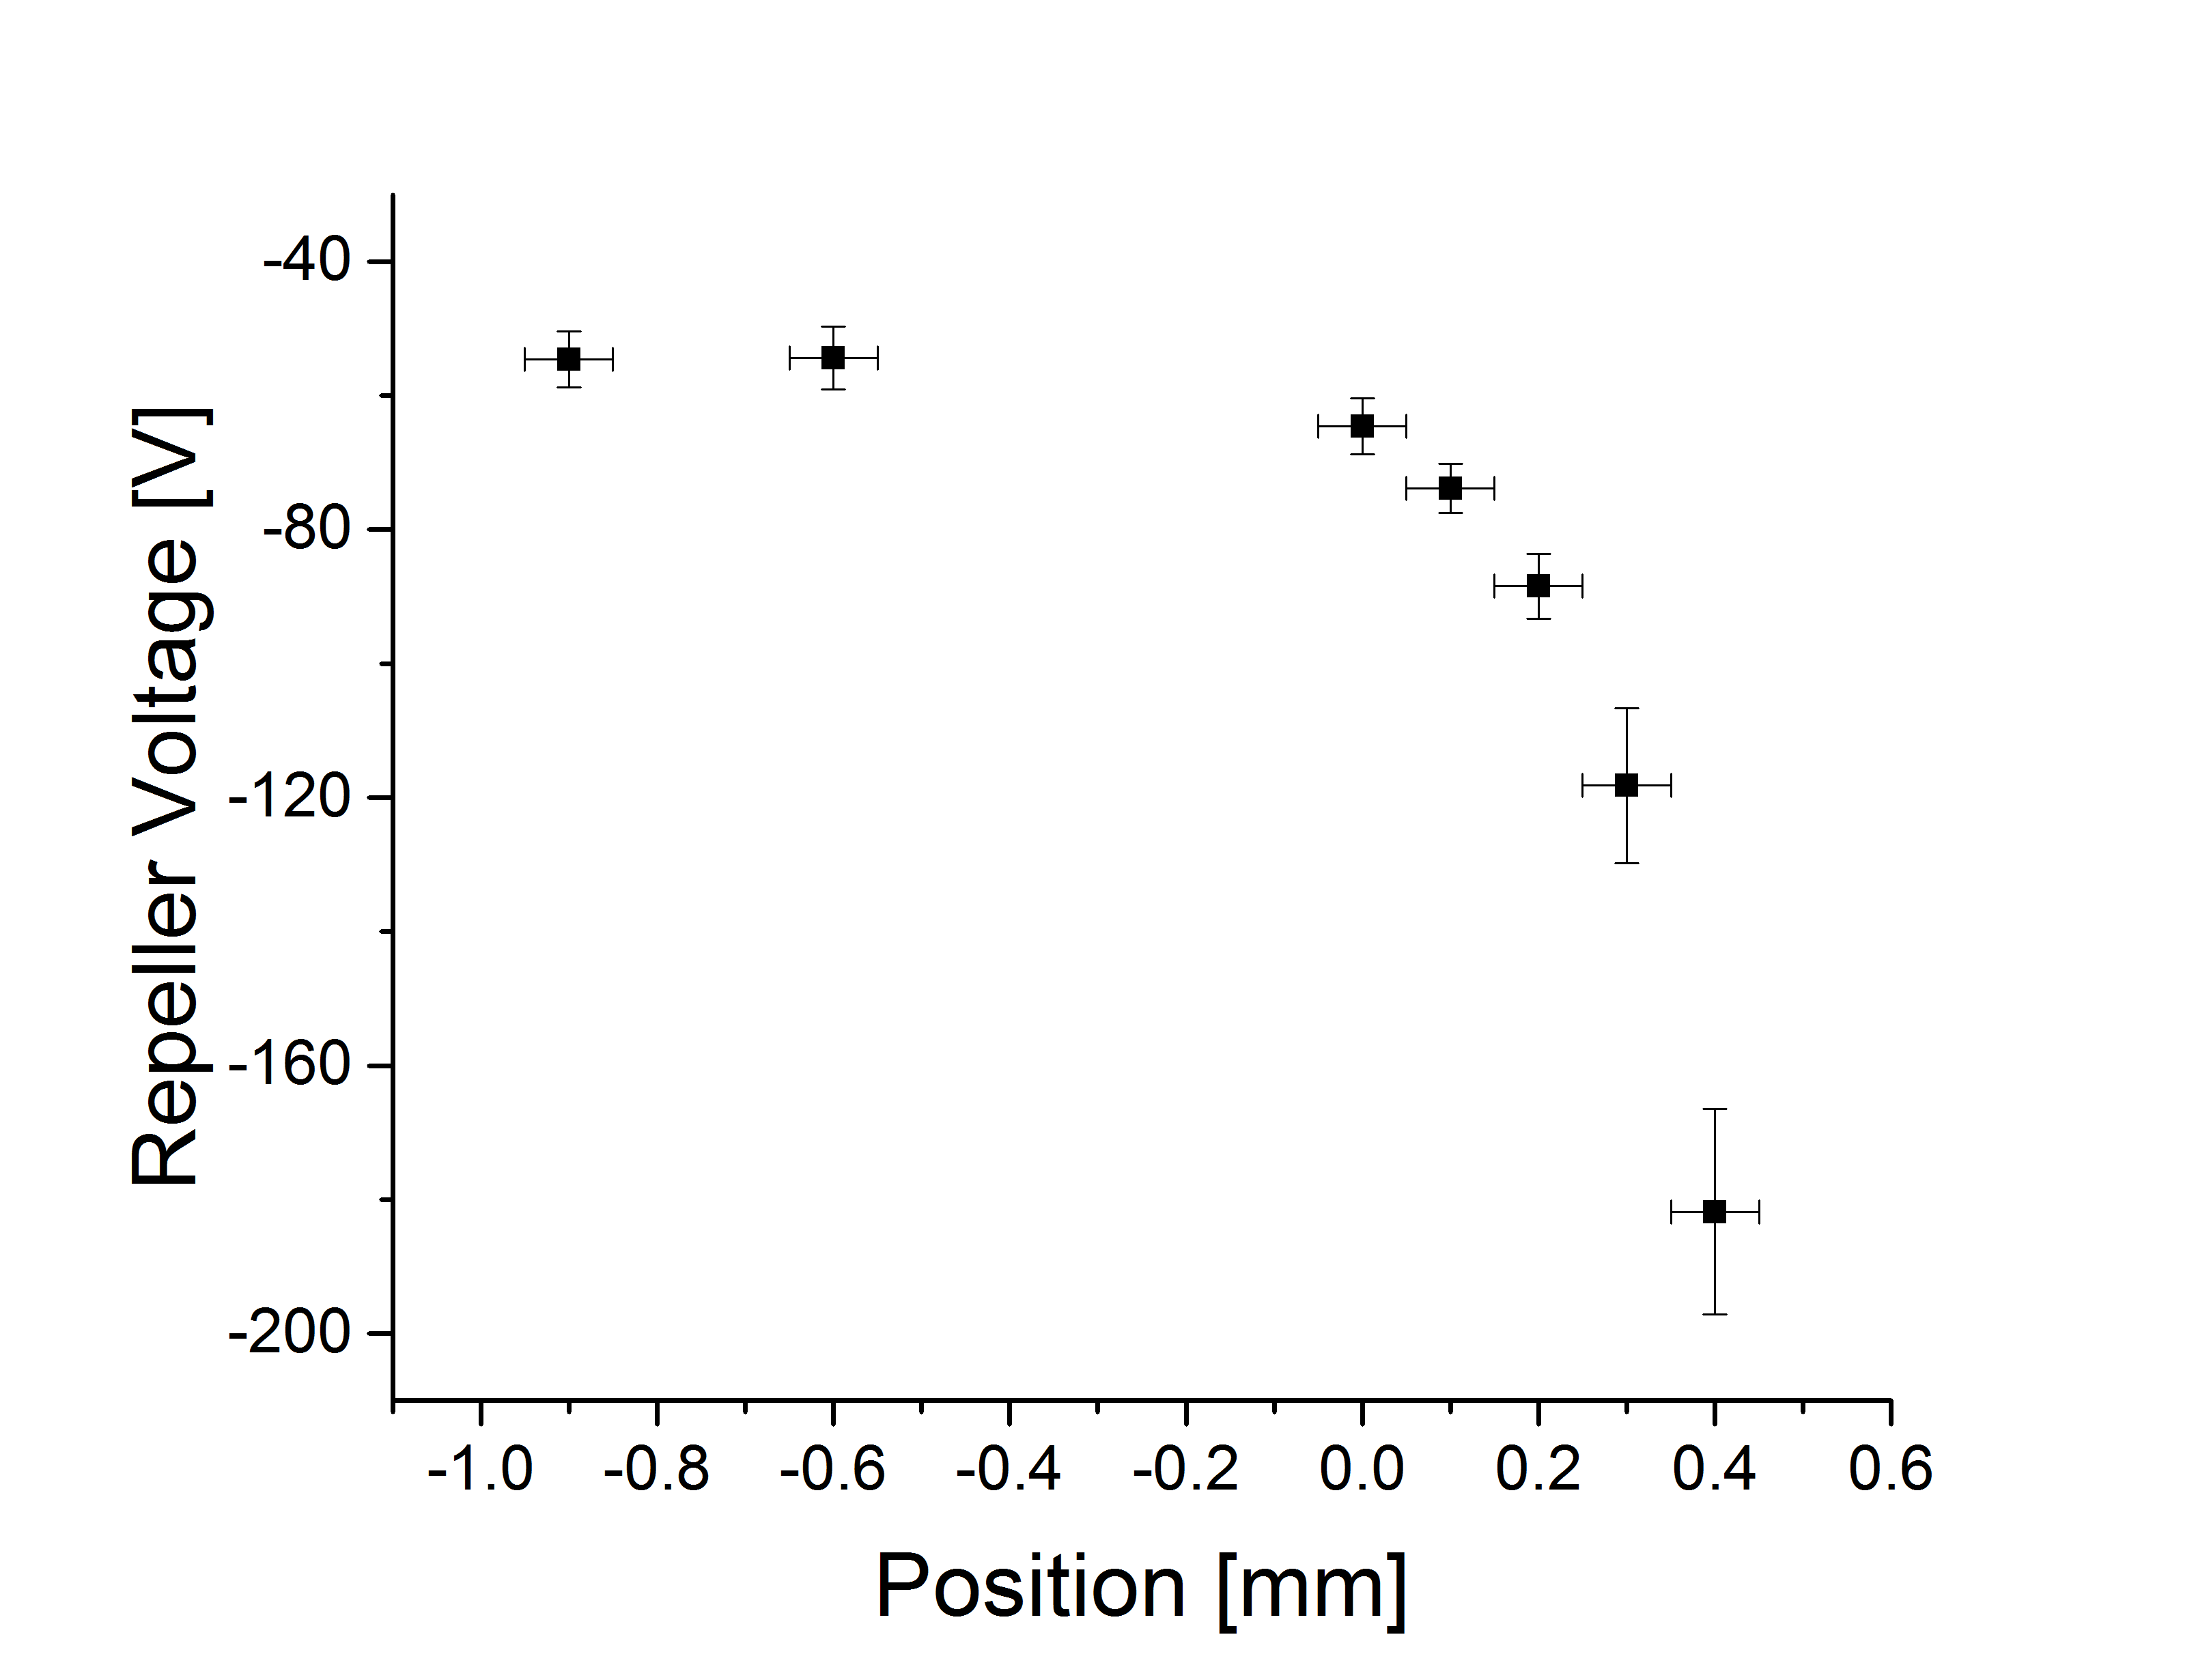
\includegraphics[width= 0.95\textwidth]{Experiments/SimRepPosU.png}
		\end{subfigure}
		\begin{subfigure}{0.47\textwidth}
			\centering
			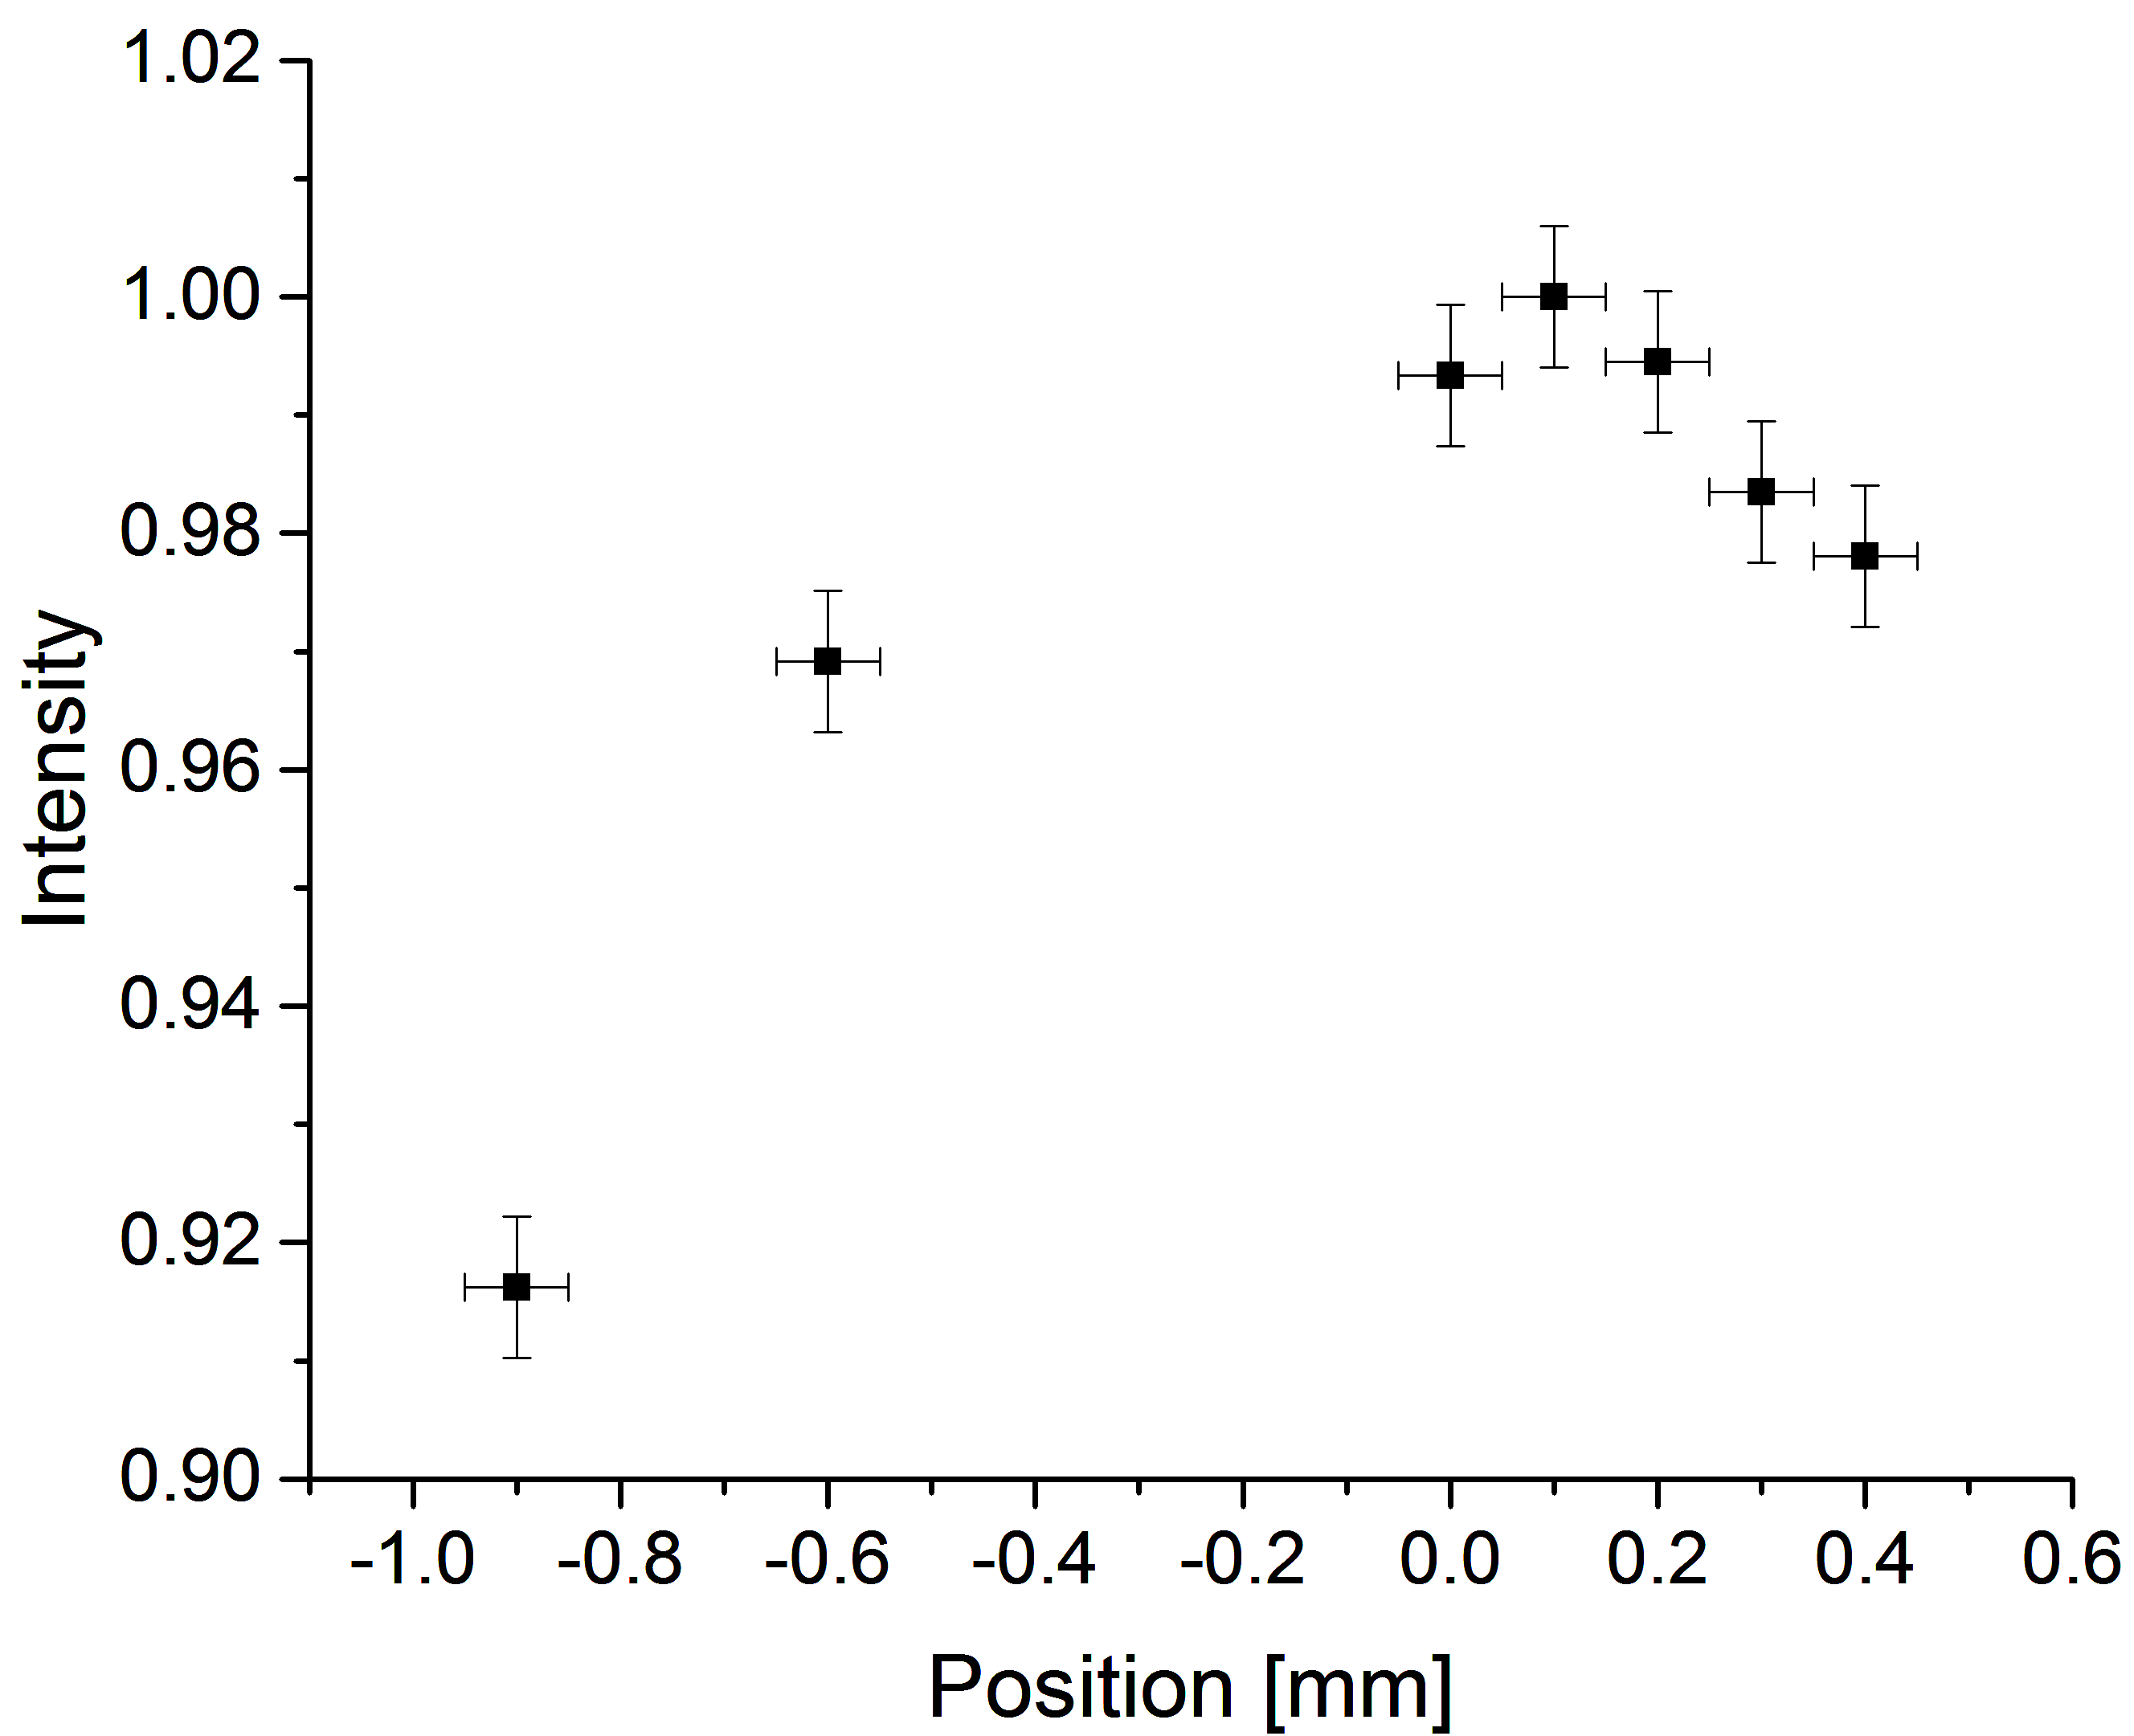
\includegraphics[width= 0.95\textwidth]{Experiments/SimRepPosImax.png}
		\end{subfigure}
		\caption{Left: The filament repeller voltage to reach the maximum electron intensity over the volume of the neutral particles. Right: Electron intensity normed on the intensity at position 0.} % Noch Graphik wie Intensität bei den versch. Pos abfällt.
		\label{fig:ExpSimRep}
	\end{figure}

	\subsection{Filament decision}
	% Ranking criterion -> Explanation, see electronics book. constant power of one filament -> resistance variies over time. Vgl. Diss Rico.

%------------------------------------------------------------------------------------
	\subsection{Pulser}
	% Simulations with different rise times and their influence on the mass spectrum.
	% Test with lab pulser, wavelab pulser -> compare their properties and their performance.
	
	% Pulsertests, Messungen, Simulationsresultate
	% Two different pulsers properties, pulse shape. Tests with different gases. Massresolution, Intensity relation?, SNR? Are these two properties correlated? Noch mit Peter anschauen. Ar sieht in allen 4 Fällen etwas komisch aus. Higher signal intensity -> higher SNR.
	% Achsenskalierung anschauen von Areagraphik. Wenn das geklärt ist, evt. in Matlab schreiben. Zusätzliches Skript für diese Graphiken, Stefans Vorlagen anschauen. Die signal intensity lässt sich nicht einfach in Druck umrechnen. Zu viele unbekannte Komponenten -> a.u. oder # e-/ns angeben.
	
	
	
	\subsection{Detector Tests}
	% FS IsoArea. Variation of the MCP gain an observation how the SNR and IsoArea change. \\titania.unibe.ch\UserHomes\foehn\MyDocuments\PhD\Messungen\FS\ firstOpti\MCP_Gain.opj
	% Also show different signal heights/ forms? Defect diode, functioning diode, resistor? Full gain curve is only possible for functioning diode (tests to be done) and resistor (plot already included).
	The following chapter describes improvements of the mechanical and electrical design of the NIM PFM detector and tests performed with different versions. Most of the tests were performed in the Pumpstand nr.2 (Chapter \ref{subsubsec:SetFacPumpst}) and a few were done with the detector in the sensor Proto Flight Model (PFM) or in the sensor flight spare model (FS).\\
	% Leave this part here as it is a description of the process we were working on. Describe the adaption of the meachanical design of the detector housing, the consequence that we inserted a resistor instead of an anode. Pros and Cons of the Anode vs. the resistor?
	% Description of the housing and problems related to it -> investigation, improvements.
	The detector suffered repeatedly discharges causing a failure of the diode, which is one of the key components of the detector. This lead to a redesign of the detector housing and to an exchange of the diode through a resistor, because the resistor is more robust concerning discharges. % Include an electrical schema. May a zoom of the other one laready included in the setup chapter (as soon as it is finished). Explanation about how a diode works? Talk with JoGa maybe. Explain main hypothesis why it died repeatedly?
	The discharges could be eliminated by a redesign of the detector housing. % Vgl. Fig. of the 2 housing designs (start and end) and explain them.
	Fig.bla left shows an earlier version of the detector housing and Fig. bla right shows the design of the current flight detector.
	Basically, the MCPs lay on a border about 1 mm above the anode. % Check distance
	A diode generates an additional voltage difference between the MCP backside and the anode to accelerate the electrons from the MCP backside towards the anode. Between this border and the MCP is the contact lug which is connected to the high voltage rail. On top of the upper MCP is the contact lug to connected to the corresponding voltage rail. On top of that is a bushing and a sort of screw. When tightening the screw, the bushing presses uniformly on the MCPs. In the old design, the thread for the screw was cut down to the boarder on which the MCPs lay. When assembling the whole stack, the MCPs often cant in the thread. Another challenge lay in tightening of the screw. When the screw was too loose, the top and the bottom contact lug had no reliable contact to the MCPs. When applying a high voltage over the whole MCP stack, the gap acts as an additional resistor over which the voltage build up resulting in a discharge between the corresponding electrode and the MCP. The discharge can propagate through the whole MCP stack and damage the diode and the capacitors. When the screw was tighten too much, the MCPs broke as they consist of lead glass and are very delicate in the mechanical point of view. As a consequence, the screw thread was cut less deep down and an additional boarder was made on which the bushing was pressed by the screw to make the assembly of the detector easier. In addition, the diode was exchanged through a resistor because the resistor is more robust in regards to the discharges. Due to the uncertainty in the manufacturing process of the detector housing, spacer rings are added between the bushing and the MCP to really close the gap. Due to that uncertainty, the number of rings needed for each detector has to be determined by trial.
	% Insert a Figure of the housing. Further explanation of the design
	% free play = thechnisch für Spiel
	% Circuit diagram with both options diode and resistor. Ref for that statement?
	% Upgrade SNp6.
	
	% Explanation of the different meas Figs.
	% Detector with broken anode is detector EM4. Look if there are any specifications. Seems to have most probable the same configuration as the other detectors. -> Sufficient for the data analysis but it would be good to have the datasheet.
	Fig. bla shows the signal shapes of different detector configurations beginning with the shape of a detector with a broken diode. The other two figures show the signal shape of a detector with a functioning diode and a functioning resistor. The most remarkable feature is that the signal height of the detector is much smaller and much broader that the signal shape of the other two configurations. In addition, the first overshoot is much lager due to the impedance mismatch caused by the broken diode. A broken diode gets conductive and therefore the potential at the MCP backside is equal to the potential of the anode. The electrons are not additionally accelerated and therefore the resulting signal is smaller than the signal with a functioning diode.\\
	Fig.\ref{fig:SN4p54p7Gain} shows the gain curves of two potential FS detectors both in the configuration with a 10\,\si{\mega\ohm} resistor instead of a diode. 
	% Other parameters to analyse? Pulse width of the 3 configurations? Overshoot? Can that really be calculated out of the data? Impedance match based on the overshoot.
	\begin{figure}
		\begin{subfigure}{.5\textwidth}
			\centering
			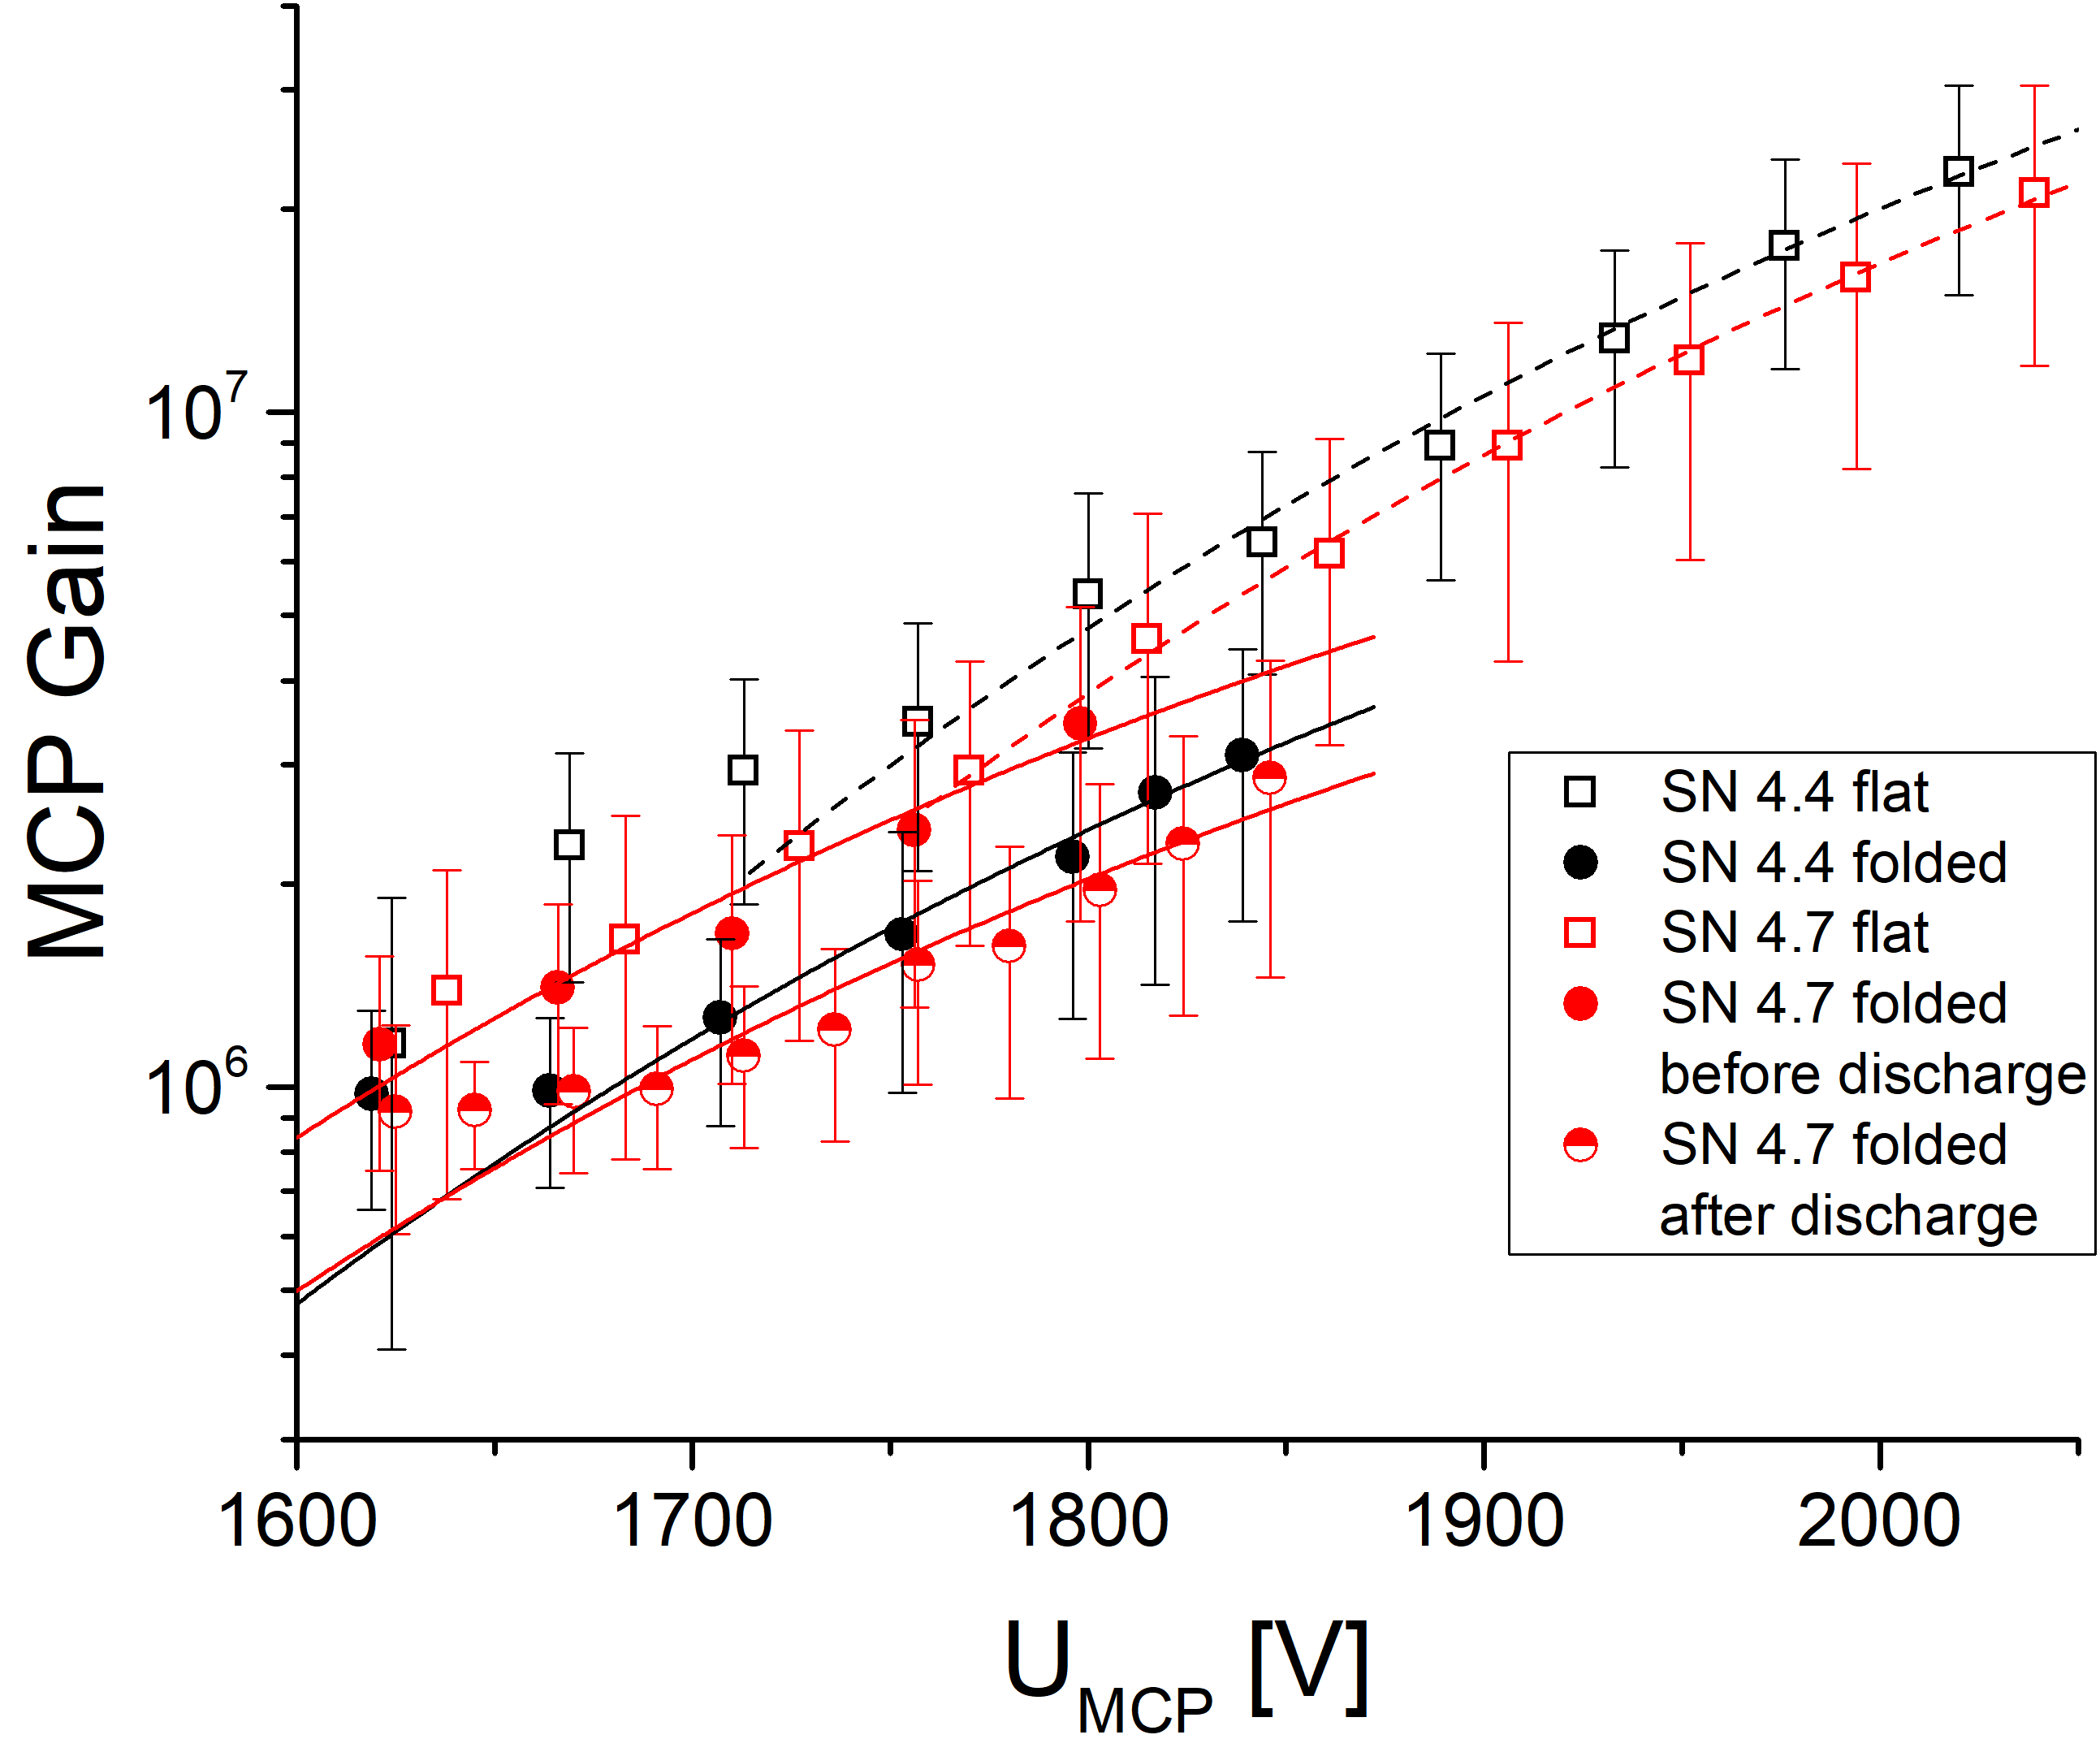
\includegraphics[width=0.9\textwidth]{Bilder/Gain_Curves_SN4p5_4p7.png}
		\end{subfigure}
		\begin{subfigure}{.5\textwidth}
			\centering
			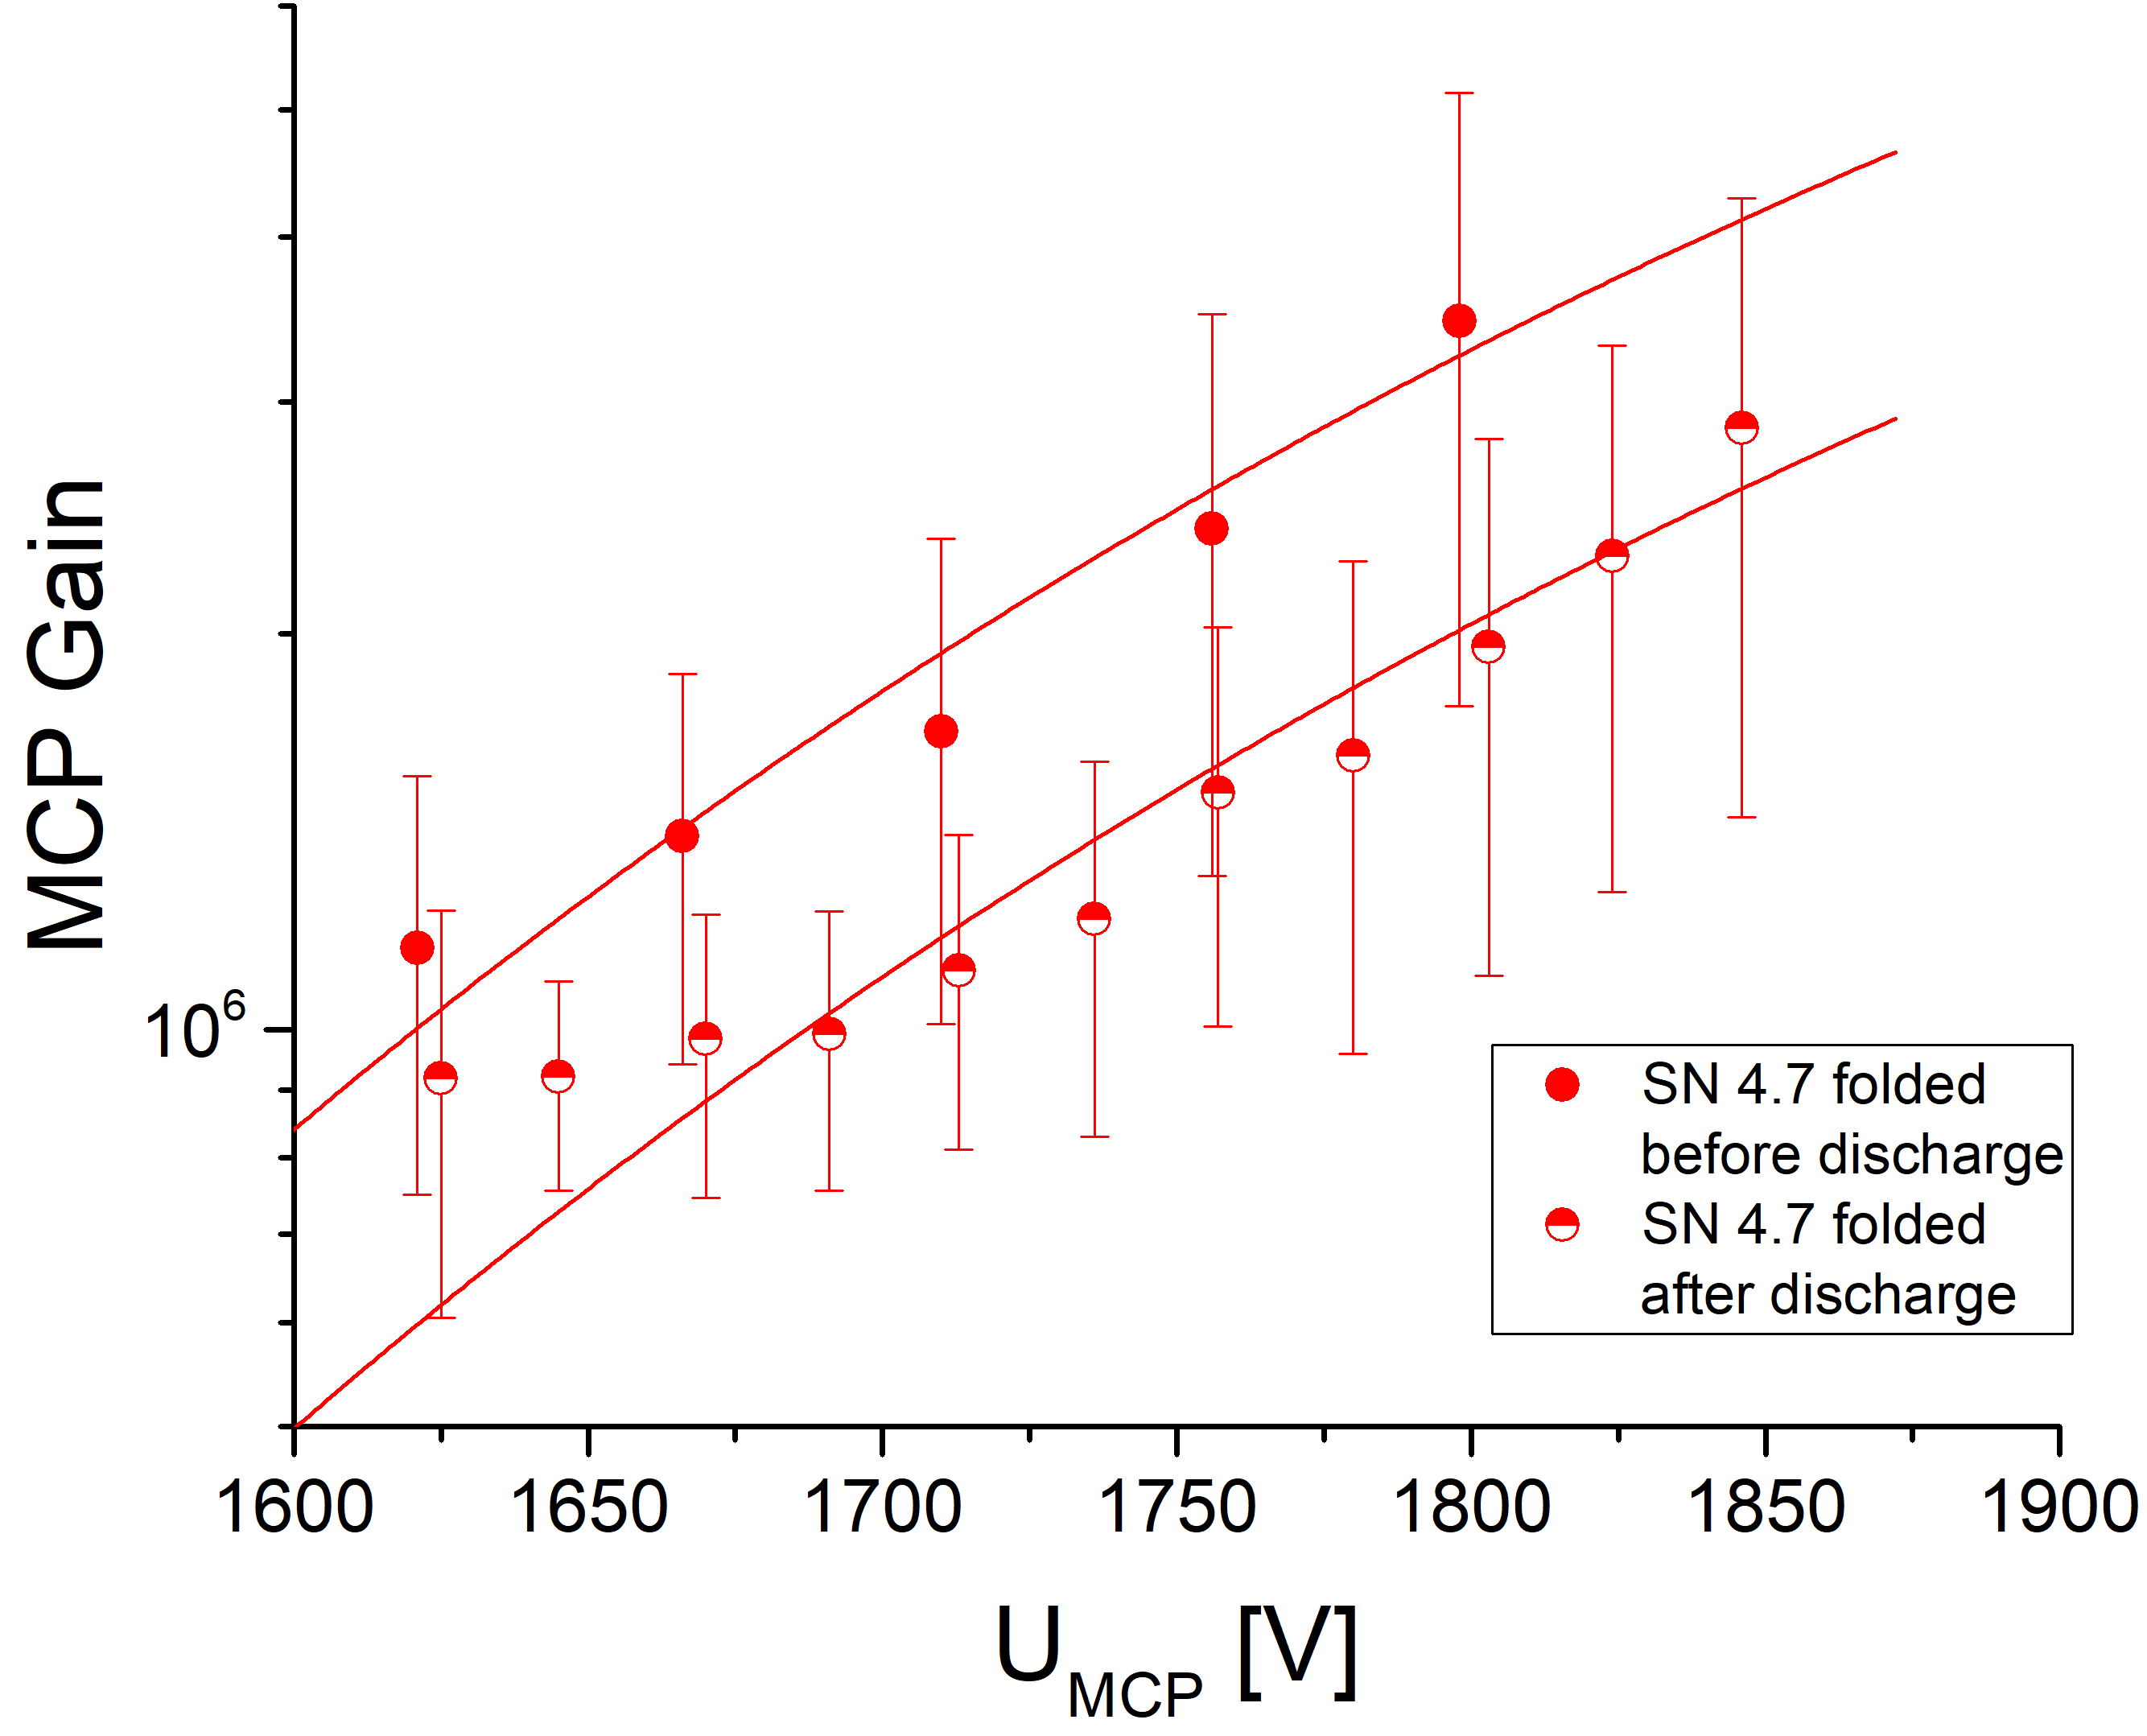
\includegraphics[width=0.9\textwidth]{Bilder/SN4p7_discharge.png}
		\end{subfigure}
		\caption{Left: Gain curves of two NIM PFM detectors. The difference in gain is because for each measurement curve, a different set of MCPs was used. Right: Gain curves of a folded NIM PFM detector. The lower gain curve was recorded after a discharge at an MCP voltage of 1.8\si{\kilo\volt}.}
		\label{fig:SN4p54p7Gain}
	\end{figure}
	% Discussion about the discharge behaviour in regards to gain. Are there any values? Something with free electrons destroying the inner coating of the MCP channels. Only a rough estimate needed.
	% Explanation of the fit model in theory part. -> Maike if there is any theory about that topic specifically.	
	
	% ROSETTA? When was a resistor latest used? Have a look if there is a space for sort of improvements of the sensor. If it is part of the experiments of of the thery part...
	% Explain, which measurements were made with which MCPs, describe how the discharge influences the signal. How much of the signal we loose in this specific measurement. Literature references?
	% Description of the current measurement of the detector with the laboratory electronics attached and then the calculation of the MCP voltage. State clearly under with circumstances the calculation with this method is possible and under which it is not (ion current, which is falsely taken into account)
	% Precise can we estimate the numbr of ions/ the partial pressure of the gas?
	% Describe, how far we tried to approximate the voltage.
	
	% Plot off the gain curves of the detector in its different states. flat, folded, folded in the wolfram copper shealding.
	% Measuring settings. Turn the drift voltage up to -2.5 kV and then slowly increase the anode voltage to the value you want to measure. The gain is calculated with the software by doing a Simpson 3/8 integration of the peak = Q. (Look in the lab book for the proper calculation)
	% Maybe there is time to redo the tests with the real PFM detector (XD wär schön. Leider nein). (Die Resultate sind nicht so vollständig wie die von der einen anderen Messung. Messung mit einem Zwillingsdetektor und von diesem auf den Flugdetektor schliessen. -> evt. schöne Graphik).
	
	
%-----------------------------------------------------------------------------------
	\subsection{Ionoptics}
	\subsubsection{Voltage Optimisation}
	Two types of electrical lenses. positive and negative voltage lenses. positive and negative voltage lenses have the same effect. In negative voltage lenses, the particles fly faster = shorter time-of-flight. This results in a better mass resolution.\\
	Aim in the lab is to get two different voltage sets. One for positive voltages to not stress the equipment and one with negative voltage lenses to reach the maximal performance of the instrument. -> Tests showed no significant better mass resolution. A more detailed data analysis has to be made. % data in folder: \\titania\UserHomes\foehn\My Documents\PhD\Messungen\PFM\CASYMIR-C\nMode_voltageSet_Comparison_200430 
	
	\subsection{Instrument performance tests}
		% At the end, make a comparison of the discussion of the different instruments as mass resolution, SNR as far as possible.
		\subsubsection{Prototype} % Final results. Only shpw best mass resolution achieved. May revere to Stefan's Diss. With the Prototype there were mainly componenets tests. Only discussion of the antechamber performance if it is not discussed in the chapter above.
		\subsubsection{PFM} % Include here the paper because it give a very good overview over the results conducted with it.
		\subsubsection{FS} % Include here the final results of the FS of this year with lab and flight electronics. Discussion about that subject, see PFM paper.
		% Laboratory and flight electronics are part of the same chapter because with the fligh electronics the only thing worth to discuss is the mass resolution because the signal intensity is still very low. Discuss the SNR graphics with Peter and then finalize this part of the chapter.
		
		% Look up the conditions for the description.
		\textbf{Ion Storage two different velocities}\\ % Ref. to Abplanalp paper.
		Ion storage is very crucial for a time of flight mass spectrometer because every ion generated and not stored in the ion source is lost and can generate additional electrical noise on the detector signal line. In this test the ion storage behaviour of the ion source was analysed for thermal and neutral mode for hydrogen and krypton with velocities of 2\,\si{\kilo\meter\per\second} and 4\,\si{\kilo\meter\per\second}. The emission current was varied from 20 to 600\,\si{\micro\ampere}. Ion storage of positive ions in x- and y- direction is supported by the negative potential generated by the electron beam. Two ring electrodes with a positive voltage applied generate a positive potential ring to trap generated ions in y- and z- direction (Fig.\ref{fig:ExpFSFlightSenIonStorIS}). For emission currents from 20 to 600\,\si{\micro\ampere} according to Eq.\,\eqref{eq:elPotIem} the negative potential in the centre of the electron beam is -0.08-(-2.59)\,\si{\volt}. Fig.\ref{fig:ExpFSFlightSenIonStor} left shows the ion storage behaviour of the ion source of hydrogen and right the ion storage behaviour of krypton. In case of no ion storage, the relationship between the electron emission current I\textsubscript{em} and the signal intensity is linear. In case of ion storage there is a quadratic relationship between I\textsubscript{em} and the signal intensity. When measuring with the thermal mode, the particles get slowed down until they have energies in the range of 0.01\,\si{\electronvolt} and are therefore easy to trap in the potential field. In neutral mode particles enter the ionisation region directly. The kinetic energy of hydrogen for velocities between 2-4\,\si{\kilo\metre\per\sec} is 0.07-0.27\,\si{\electronvolt}. It can therefore easy be trapped in the potential field by the electron beam and the potential of the ring electrode already with very emission currents as low as 20\,\si{\micro\ampere}.\\
		The kinetic energy of \textsuperscript{84}Kr for the same velocities is 2.8-11.2\,\si{\electronvolt}. This energy exceeds the potential of the centre of the electron beam and the ions are therefore more difficult to trap with only the electron beam. The ions are kept in the middle of the ionisation region with the positive potential ring. According to Fig.\,\ref{fig:ExpFSFlightSenIonStor} ion storage for \textsuperscript{84}Kr starts to dominate at emission currents of 100\,\si{\micro\ampere}.
		%Therefore there is no difference in the measured intensities for hydrogen when it enters with 2 or 4\,\si{\kilo\meter\per\second}.\\		
		In thermal mode, an increase in beam velocity leads to an increase in signal intensity due to the density enhancement effect \textcolor{red}{(Ref.)}. Therefore a higher signal intensity is expected in thermal mode for 4\,\si{\kilo\meter\per\second} compared to 2\,\si{\kilo\meter\per\second}. 
		Like the in PFM, the FS shows a nice ion storage behaviour. For krypton ion storage just starts at an emission current of 100\,\si{\micro\ampere} where hydrogen is stored already at lower emission currents due its lower kinetic energy at the same beam velocity.
		
		\begin{figure}[h]
			\centering
			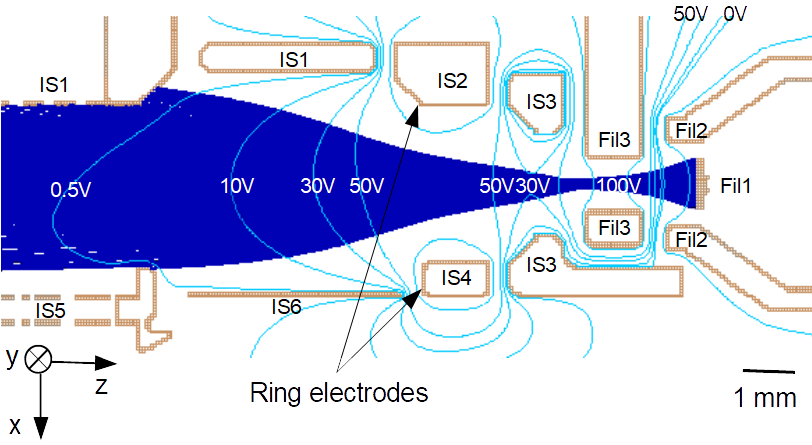
\includegraphics[width = 0.8\textwidth]{Experiments/FiL_IS_elBeam_Storage.png}
			\caption{Ion storage source with sample voltage set applied to the electrodes. In light blue are the potential lines and in dark blue a simulated electron beam.}
			\label{fig:ExpFSFlightSenIonStorIS}
		\end{figure}
		
		
		\begin{figure}[h] % Ion storage. Exchange Graphics as soon as discussed with Peter how to proper show the results.
			\begin{subfigure}{0.5\textwidth}
				\centering
				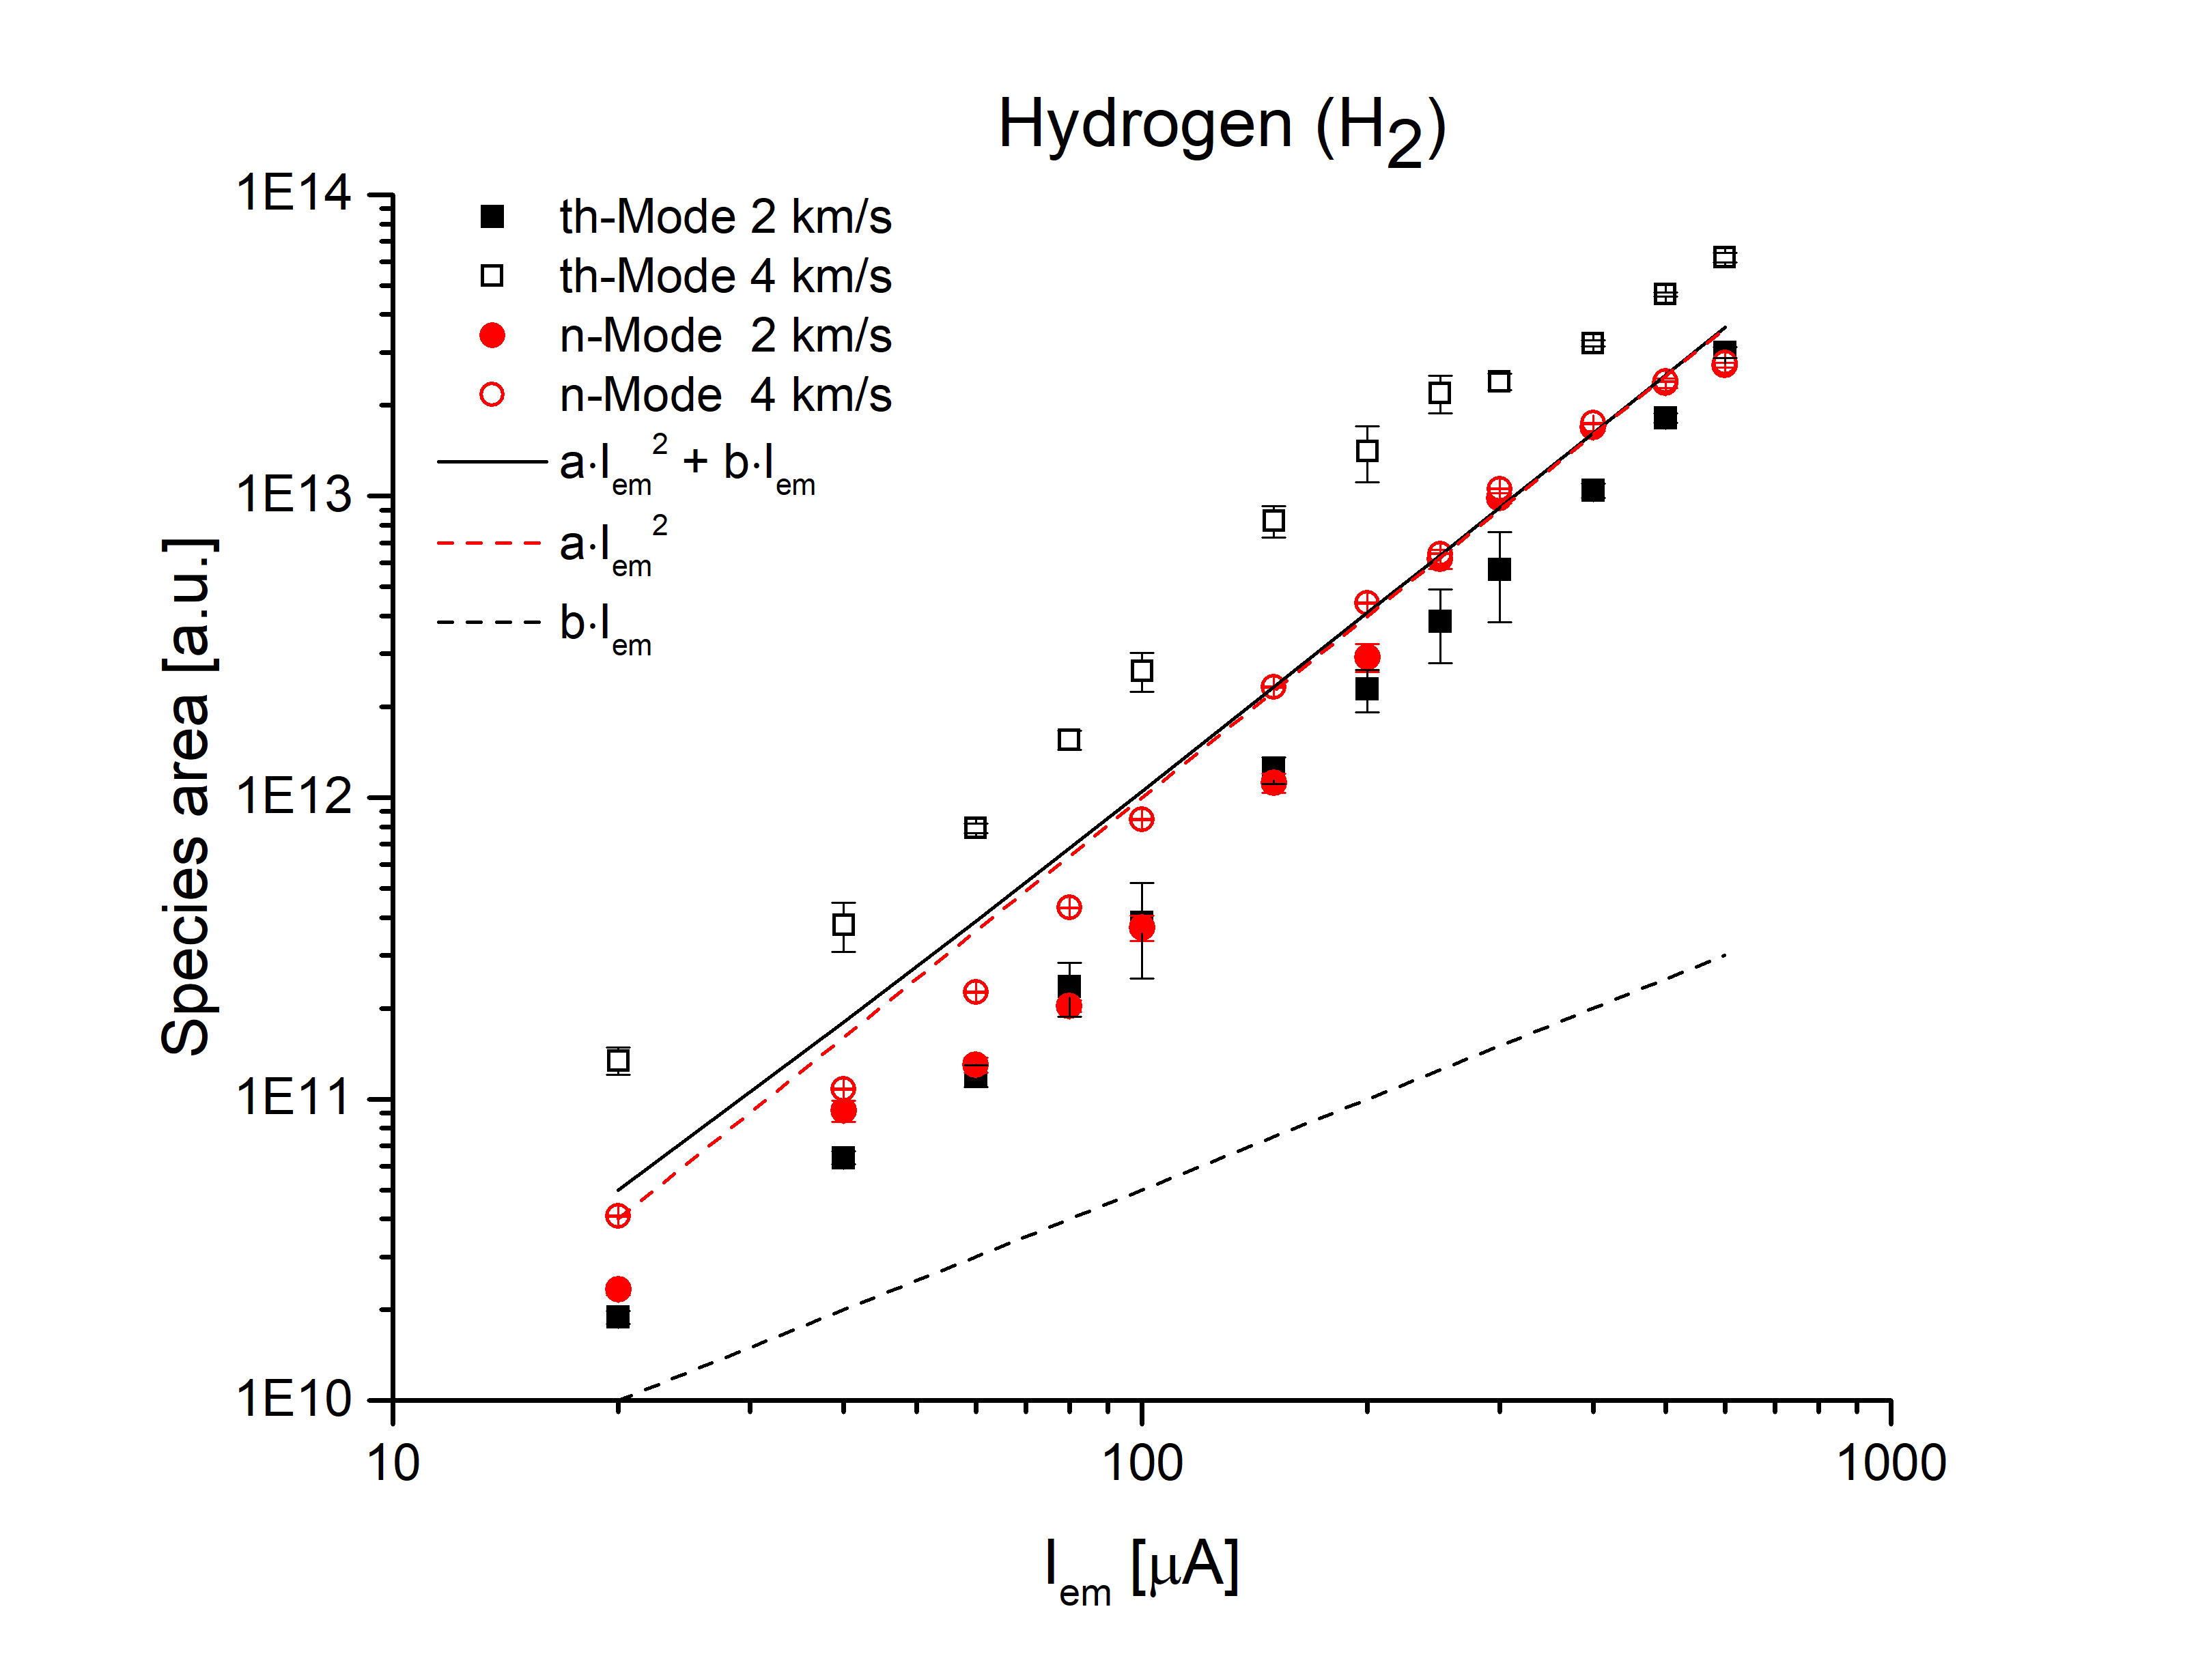
\includegraphics[width = \textwidth]{Experiments/FSLabIonStorageH2.png}
			\end{subfigure}
			\begin{subfigure}{0.5\textwidth}
				\centering
				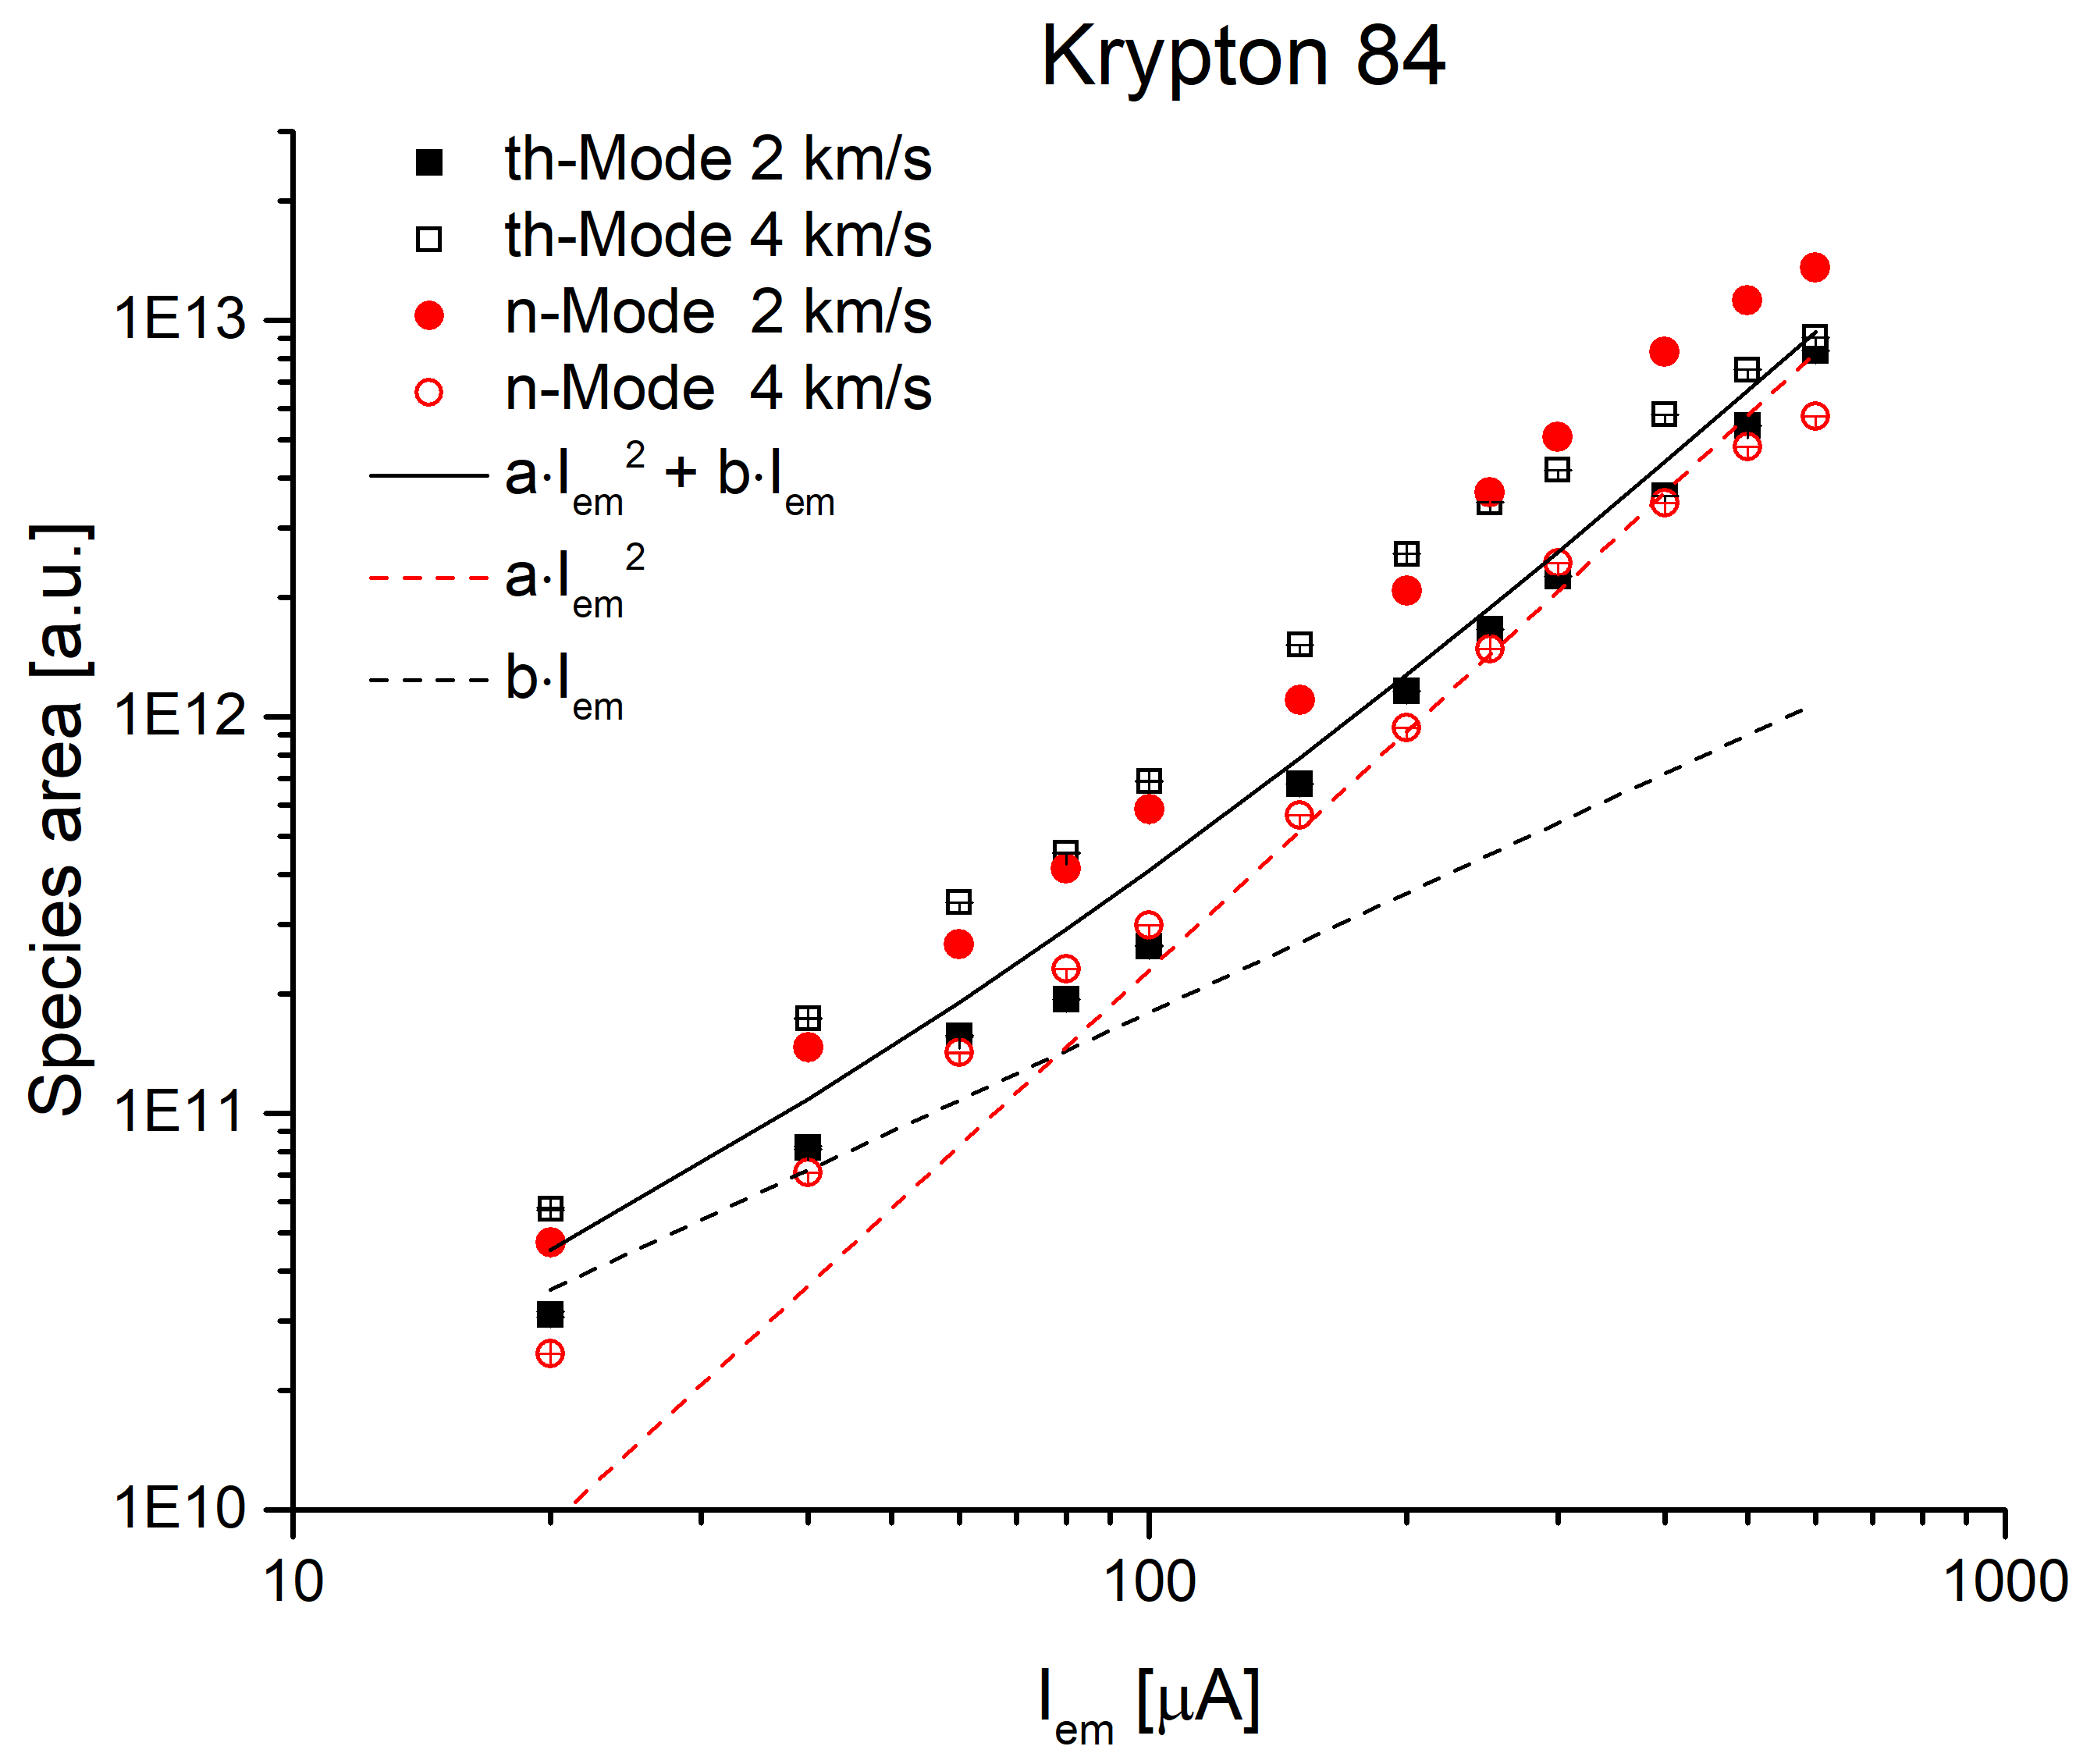
\includegraphics[width = \textwidth]{Experiments/FSLabIonStorageKr84.png}
			\end{subfigure}
			\caption{Ion storage measurement with the flight spare sensor but with laboratory electronics attached for H$_2$ and $^{84}$Kr for two different gas velocities.}
			\label{fig:ExpFSFlightSenIonStor}
		\end{figure}

		% Detector behaviour test in FS sensor. Formula derivation is in the theory part with the proper detrivation.
		% No saturation observed. 

		\textbf{Mass resolution and Signal-to-Noise Ratio}\\
		According to the requirements stated in (Ref.) % See paper
		the required mass resolution for neutral mode is 500 and for thermal mode it is 1000 m/dm but to be able to distinguish between different masses at unit masses of 1000\,u NIM has to have a mass resolution of 1000. Otherwise NIM the different unit masses cannot be distinguished. Fig.\,\ref{fig:ExpFSFlightSenMassRes} show two spectra recorded with the NIM flight sensor with laboratory electronics attached with an electron emission current of 100\,\si{\micro\ampere}. With a mass resolution of 708 for neutral gas mode NIM fulfils the requirements. In thermal gas mode the highest mass resolution achieved was 830 m/$\Delta$m which comes close to the requirements. Fig.\,\ref{fig:ExpFSFlightElMassRes} show the mass spectra recorded with the NIM flight sensor with the flight electronics attached. The electron emission current was 200\,\si{\micro\ampere} the highest mass resolution achieved at the current state is 490 m/$\Delta$m for neutral gas mode and 462 m/$\Delta$m for thermal mode. Fig.\,\ref{fig:ExpFSFlightElK78} shows a mass spectrum recorded in thermal mode with an emission current of 300\,\si{\micro\ampere} the $^{78}$Kr peak is clearly visible. The signal to noise ratio for the spectra recorded with the flight electronics is very low compared to the SNR for the spectra recorded with the laboratory electronics. We also observe noisy part wandering between the single spectra. There is a significant part of repetitive noise appearing not always at the same position in the spectrum. With a proper noise filter this noise can be detected and significantly reduced without affecting the mass signal peaks. For future work, there is a lot of potential for improving the spectrum by proper analysing the noise and writing filters to suppress the noise.\\
		Fig.\,\ref{fig:ExpFSFlightSenSNR} shows a mass spectrum recorded with the flight sensor with the laboratory electronics attached. The highest SNR achieved was $6\cdot10^{5}$ and therefore almost 6 decades. % Explanation why the 6 decades are required.
		The mass peaks 355\,u, 390\,u and 429\,u are some oil components with water adducts coming from the used turbo pumps of the test facility. 415\,u is an artefact coming from the background subtraction algorithm. The artefact peak is also wider then the other surrounding mass peaks.
		
		\begin{figure}[h]
			\begin{subfigure}{0.5\textwidth}
				\centering
				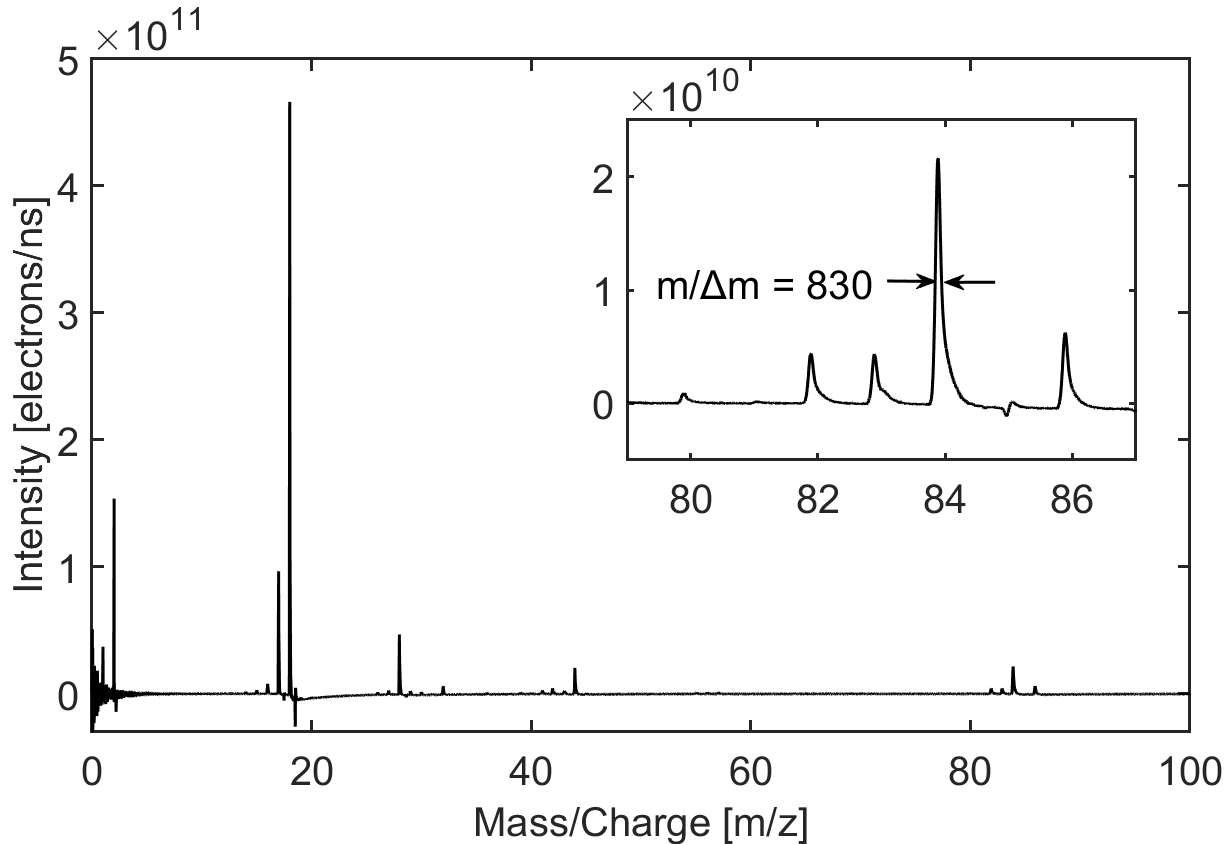
\includegraphics[width = \textwidth]{Experiments/FSLabthMode.png}
			\end{subfigure}
			\begin{subfigure}{0.5\textwidth}
				\centering
				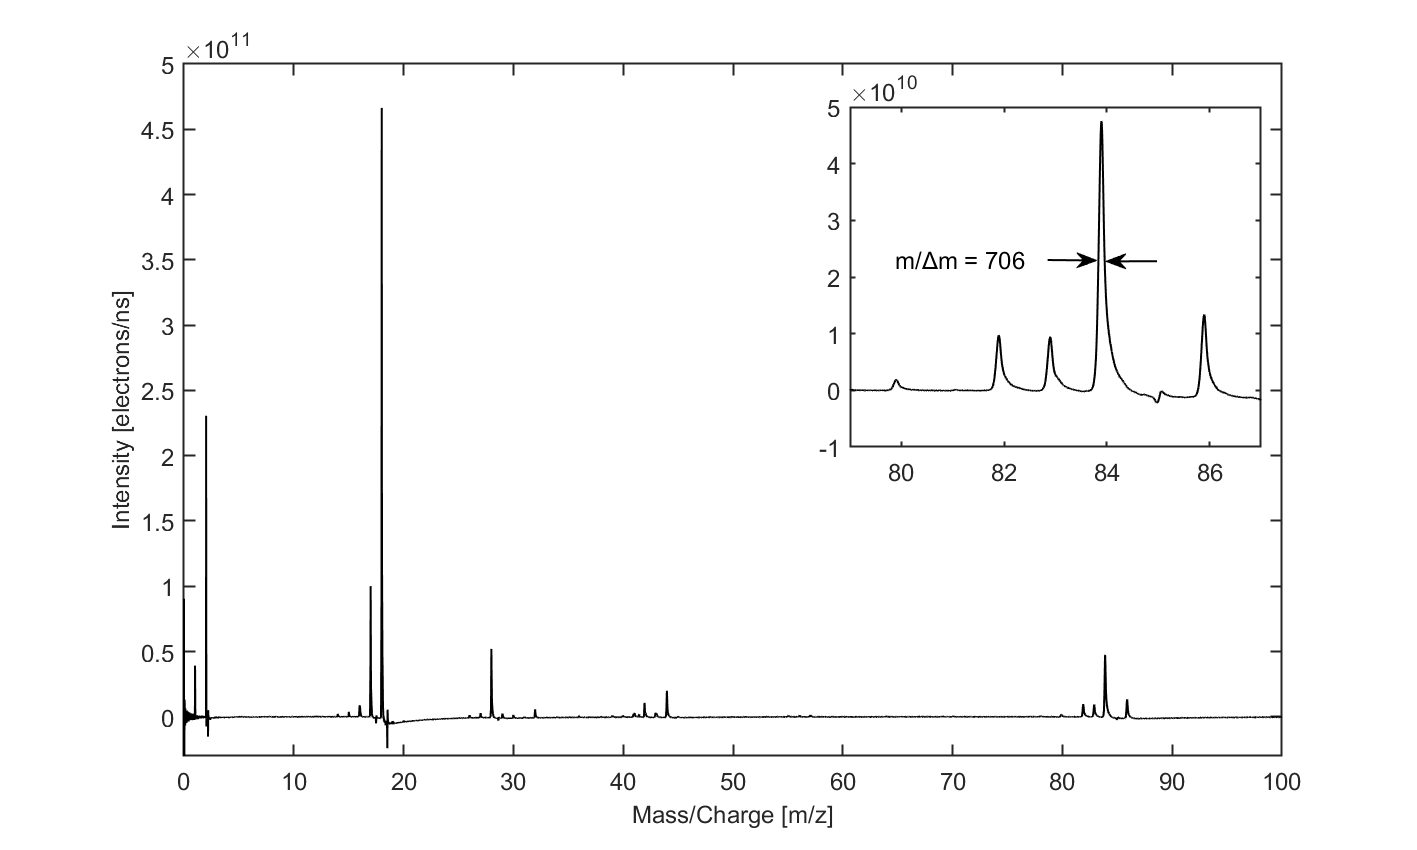
\includegraphics[width = \textwidth]{Experiments/FSLabnMode.png}
			\end{subfigure}
			\caption{Mass spectra measured with the flight spare sensor with the laboratory electronics electronics attached. Left: with thermal gas mode Right: neutral mode.}
			\label{fig:ExpFSFlightSenMassRes}
		\end{figure}

		% Mark the noisy part for better description to explain that
		% conditions: nMode UMCP: 1950 V. P = 1.03e-8 mbar 20H2:1Kr
		%			thMode UMCP = 1950 V. P = 6.05e-8 mbar
		\begin{figure}[h]
			\begin{subfigure}{0.5\textwidth}
				\centering
				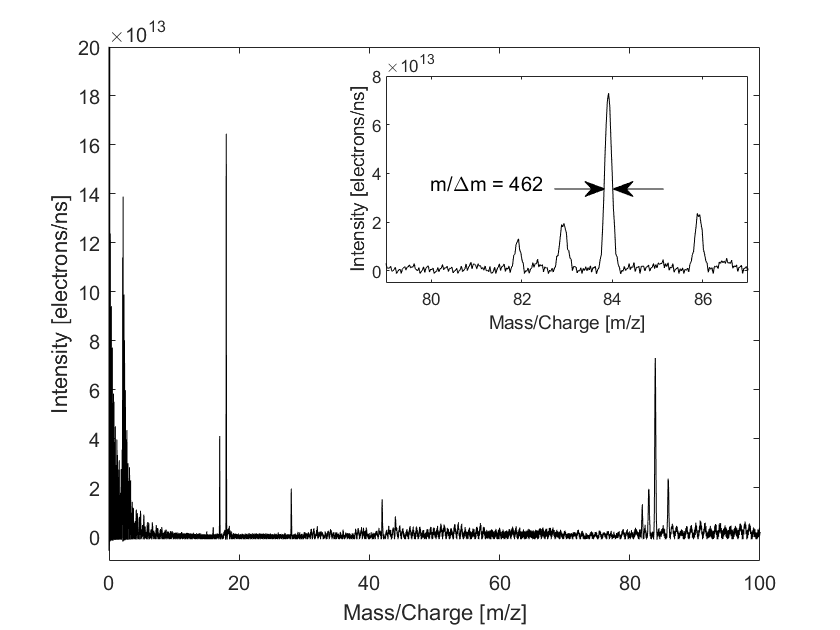
\includegraphics[width = \textwidth]{Experiments/FSthMode200uA.png}
			\end{subfigure}
			\begin{subfigure}{0.5\textwidth}
				\centering
				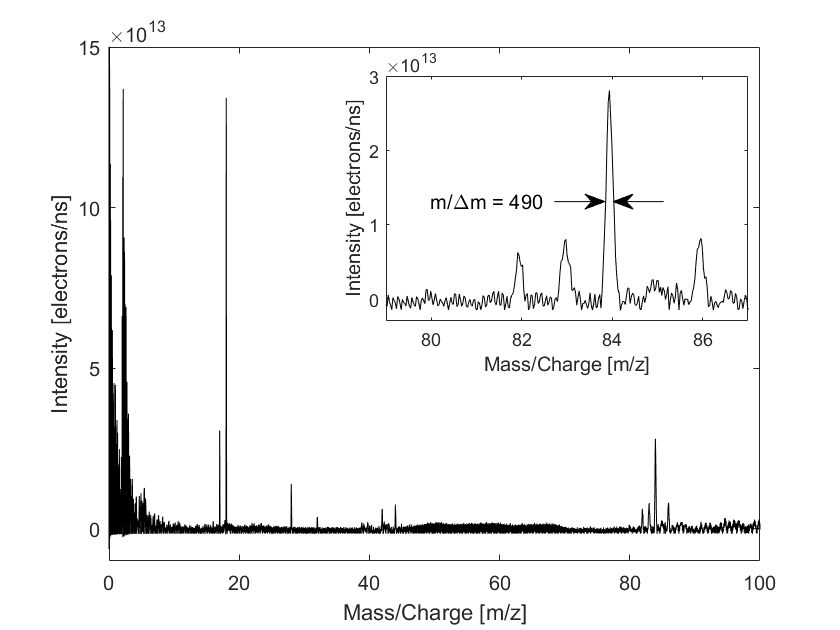
\includegraphics[width = \textwidth]{Experiments/FSnMode200uA.png}
			\end{subfigure}
			\caption{Mass spectra measured with the flight spare instrument with the flight electronics attached. Filament emission current was 200 \si{\micro\ampere}. Left: with thermal gas mode Right: neutral mode.}
			\label{fig:ExpFSFlightElMassRes}
		\end{figure}
		
		\begin{figure} % Point out at that picture that the Kr 78 isotope is clearly visible.
			\centering
			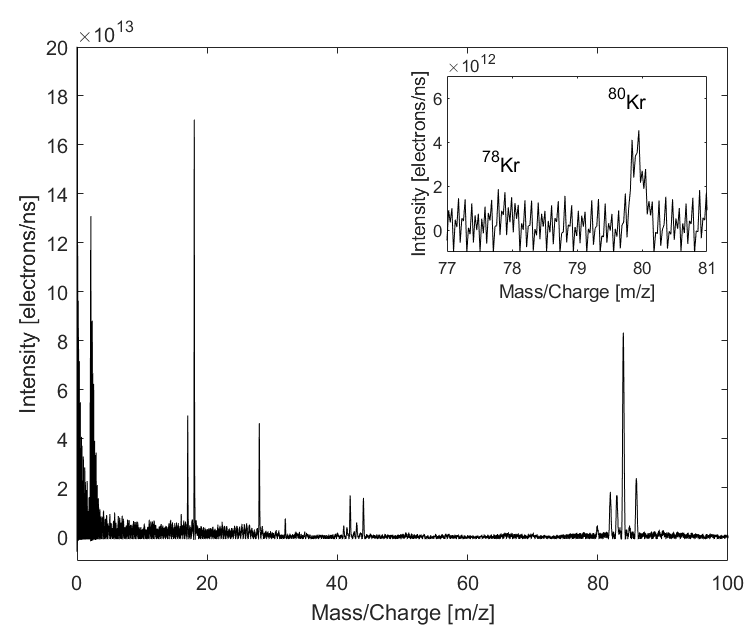
\includegraphics[width = 0.6\textwidth]{Experiments/FS_thMode300uA.png}
			\caption{Mass spectra measured with the flight spare instrument with the flight electronics attached. Filament emission current was 300 \si{\micro\ampere}.}
			\label{fig:ExpFSFlightElK78}
		\end{figure}
		
		% SNR 600 uA emission current. Rest gas Ptot = 1.6e-9 mbar, UMCPeff = 1.8 kV. Name the gas peaks. Peaks around 200 u are not mercury because the isotopic ratio does not match the pattern.
		\begin{figure}[h]
			\centering
			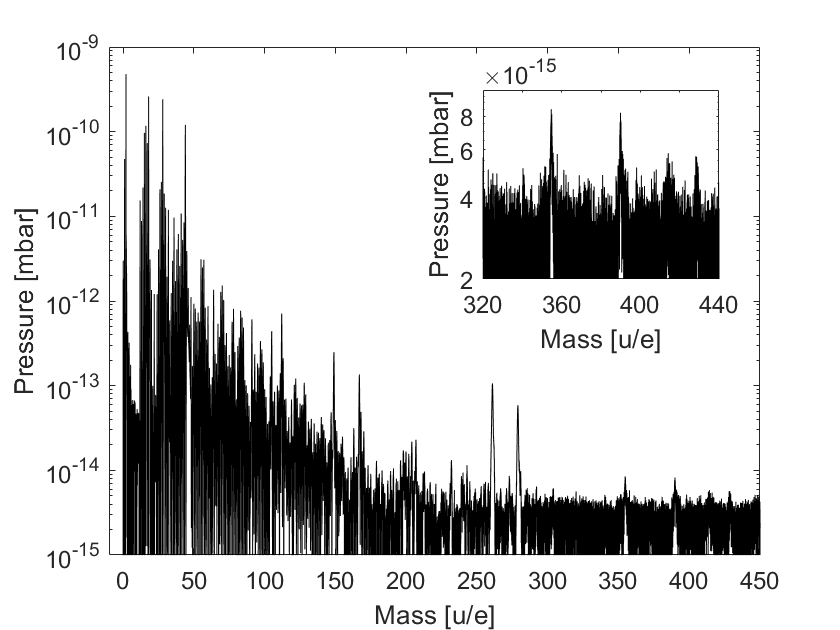
\includegraphics[width = 0.7\textwidth]{Experiments/FSLabSNRRestGasPressCal.png}
			\caption{SNR plot for the flight spare sensor but with laboratory electronics attached at a chamber pressure of 1.5$\cdot10^{-9}$\si{\milli\bar}.}
			\label{fig:ExpFSFlightSenSNR}
		\end{figure}
	
	
	
	
	
	
	 % Sämtliche Experimente/ Tests einmal da rein unter der Annahme, dass das Instrument schon beschrieben wurde. Wichtige Teile, welche ins Setup gehören gleich eine Notiz in Setup machen.
	\clearpage
	% !TEX root = arbeit.tex
\section{Conclusion}

	% Wichtigste Punkte nocheinmal zusammenfassen. Evt. auch die Conclusions der Papers hier nochmal kurz erwähnen.
	\newpage
	\thispagestyle{empty}
	\null
	\newpage
	% !TEX root = arbeit.tex
\section{Outlook}
	
	The NIM PFM was successfully delivered to the JUICE spacecraft in December 2020 and at the current state, the NIM FS model waits until the JUICE spacecraft started its journey to Jupiter in September 2022. Until then, the FS waits as it is the spare model for the case that something happens to the PFM on the spacecraft until launch. After the start of the spacecraft, the NIM FS has to be properly calibrated with the actual flight electronics. Most results presented in this thesis were conducted with laboratory electronics attached to the two sensors because there was only very little time to test the whole system. The NIM ion-optical system was first qualified as a separate unit and now there follows the calibration of the whole NIM instrument.\\
	In addition, the flight software is still under development and has to be tested with the full system. The optimizer to optimized the voltage sets during the flight is still under development. As soon as it is available for tests, it has to be tested and the target function used to improve the voltage sets has to be adapted for NIM. First results of the FS sensor operated with flight electronics revealed that there lies a lot of potential in the postprocessing of the data especially in regards to filtering. Therefore a proper filter has to be written to improve the SNR of the final spectra.
	
	% SATANS with Ref. and what SATANS can do
	\clearpage
	\bibliography{Quellen}
	\clearpage
	% !TEX root = arbeit.tex
\section{Appendix} \label{sec:appendix}

	% Schauen, was da alles reinkommt.
	% Startup Procedure of both filaments.
	\clearpage
	
	\section*{Acknowledgement} % Noch die alte vo der Masterarbeit
	
	My thanks go to:
	
	Prof. Dr. Peter Wurz for the opportunity to work on such a versatile experiment. The work was very instructive from the physical and the technical point of view. I also appreciated the educational discussions.
	Enduring my shenanigans.
	
	Stefan Meyer who introduced me to the work with the ILENA test facility and who had always an open ear for my questions at the beginning of this thesis.
		
	Harald Mischler and the team from the mechanic's workshop of the University of Bern and also to my office colleagues Georg Bodmer, Adrian Etter and Joël Gonseth for their technical support in the laboratory and the amusing discussions in our office.
	
	my friends with whom I had so many distracting and constructive discussions especially during our weekly coffee breaks.
	
	\newpage
	\thispagestyle{empty}
	\null
	\newpage
	
	\includepdf[pages=-]{MSc_Masterarbeit_erklaerung.pdf}
	
\end{document}




